%%-*- mode: LaTeX; mode: FlySpell; -*-

\documentclass{elsarticle}

\usepackage{amssymb,amsmath}

\usepackage{graphicx}
\usepackage{zed-csp}
%\usepackage{csp}
%\usepackage{algorithm}
%\usepackage{algpseudocode}
\usepackage{float}
\usepackage{url}
\usepackage{cite}
\usepackage{tabularx}
%\usepackage{cases}

% The line below was added as a workaround for spacing ``f'' in mathit. \mathit can now be replaced by \Lmathit to get better spacing. 
\DeclareMathAlphabet{\Lmathit}{\encodingdefault}{\familydefault}{m}{it}

\interdisplaylinepenalty=2500

\newfloat{algorithm}{tbp}{lop}
\floatstyle{ruled}

\newtheorem{lemma}{Lemma}%
\newtheorem{definition}{Definition}%
\newtheorem{conjecture}{Conjecture}%
\newtheorem{theorem}{Theorem}%
\newtheorem{proposition}[theorem]{Proposition}

% include if zed-csp is not included.
% \newcommand{\hide}{\setminus}
% \newcommand{\spot}{\bullet}

%include if zed-csp IS included.
\renewcommand{\inv}{\mathit{inval}}
%otherwise
%\newcommand{\inv}{\mathit{inval}}

\newcommand{\prov}{\mathit{prov}}
\newcommand{\dep}{\mathit{dep}}
\newcommand{\pr}{\mathit{pr}}
\newcommand{\obf}{\mathit{abs}}
\newcommand{\pol}{\mathit{pol}}

\newcommand{\pg}{\mathit{PG}}
\newcommand{\en}{\mathit{En}}
\newcommand{\act}{\mathit{Act}}
\newcommand{\ag}{\mathit{Ag}}

\newcommand{\used}{\Lmathit{used}}
\newcommand{\wgby}{\Lmathit{genBy}}
\newcommand{\influence}{\Lmathit{wasInfluencedBy}}
\newcommand{\wdf}{\Lmathit{wasDerivedFrom}}
\newcommand{\waw}{\Lmathit{waw}}
\newcommand{\attrTo}{\Lmathit{wat}}
\newcommand{\wat}{\Lmathit{wat}}
\newcommand{\delegate}{\Lmathit{abo}}
\newcommand{\wasInfBy}{\Lmathit{wasInformedBy}}
\newcommand{\start}{\Lmathit{start}}
\newcommand{\ed}{\Lmathit{end}}


\newcommand{\Ev}{\mathit{Ev}}
\newcommand{\preorder}{\preceq}

\newcommand{\evmap}{\mathit{evmap}}


\newcommand{\node}{\mathit{Node}}
\newcommand{\type}{\mathit{type}}
\newcommand{\elabel}{\mathit{label}}

\newcommand{\guEA}{\pg_{gu/ea}}  % gen-usage over enties, activities
\newcommand{\guiEA}{\pg_{gui/ea}}
\newcommand{\guaEAG}{\pg_{gu+/eaAg}}  % gen-usage and more over enties, activities plus Agents

%% operators
\newcommand{\group}{\mathit{Group}}
\newcommand{\aggroup}{\mathit{agGroup}}
\newcommand{\sgroup}{\mathit{Group_{str}}}
\newcommand{\clos}{\mathit{pclos}}
\newcommand{\repl}{\mathit{replace}}
\newcommand{\agrepl}{\mathit{agreplace}}
\newcommand{\rewire}{\mathit{rewire}}
\newcommand{\extend}{\mathit{extend}}
\newcommand{\pclos}{\mathit{pclos}}
\newcommand{\rem}{\mathit{remove}}
\newcommand{\agremove}{\mathit{AgRemove}}
\newcommand{\orphanremove}{\mathit{OrphanRemove}}
\newcommand{\allorphanremove}{\mathit{AllOrphanRemove}}
\newcommand{\remIsolated}{\mathit{remIsolated}}

\newcommand{\dclos}{\mathit{dclos}}

\newcommand{\POL}{\mathit{\cal P}}

%\newcommand{\mnote}[1] {\marginpar{\scriptsize \raggedright #1 }}
\newcommand{\mnote}[1] {  \framebox{\begin{minipage}[t]{0.9\linewidth}
 \scriptsize \raggedright #1 \normalsize
    \end{minipage}
 }}

\newenvironment{mydrop}{\begin{array}[t]{@{}l@{}}}{\end{array}}%



\usepackage{color}
\usepackage{pdfpages}
\usepackage{ifthen}
\newcommand{\showColour}{yes} % {yes}
\newcommand{\showComments}{yes} % {yes}
\newcommand{\note}[2]{\ifthenelse{\equal{\showColour}{yes}}{\textcolor{#1}{#2}}{#2}}
\newcommand{\jwb}[1]{\note{blue}{#1}}

\newcommand{\paolo}[1]{\note{magenta}{#1}}


\newcommand{\com}[2]{\ifthenelse{\equal{\showComments}{yes}}{\textcolor{#1}{#2}}{}}
\newcommand{\comment}[1]{\com{red}{#1}}



\begin{document}

\title{Abstracting PROV provenance graphs: a validity-preserving approach}


\author[ncl]{P. ~Missier \corref{cor1}}
\ead{Paolo.Missier@newcastle.ac.uk}

\author[cov]{J. ~Bryans\corref{cor2}}
\ead{Jeremy.Bryans@coventry.ac.uk}

\author[ncl]{C. ~Gamble}
\ead{Carl.Gamble@newcastle.ac.uk}
    
\author[kcl]{V. ~Curcin}
\ead{Vasa.Curcin@kcl.ac.uk}

\address[ncl]{School of Computing Science, Newcastle University, UK}
\address[cov]{Institute for Future Transport and Cities, Coventry University, UK}
\address[kcl]{Department of Computing, Imperial College, London, UK}

\cortext[cor1]{Principal Corresponding Author}
\cortext[cor2]{Corresponding Author \comment{I'd appreciate if we could both be ``corresponding author'' here}}

\markboth{IEEE Transaction on Knowledge and Data Engineering,~Vol.~X, No.~Y, DATE}%
{Shell \MakeLowercase{\textit{et al.}}: happy}


\begin{abstract}
Data provenance is a structured form of metadata designed to records the activities and datasets involved in data production, as well as their dependency relationships. The PROV data model, released by the W3C in 2013, defines a schema and constraints that together provide a structural and semantic foundation for provenance. This enables the interoperable exchange of provenance between data producers and consumers. When the provenance content is sensitive and subject to disclosure restrictions, however, a way of partially obfuscating provenance in a principled way before communicating it to certain parties is required. In this paper we present a provenance abstraction operator that achieves this goal. It maps a PROV document $P_1$  to a new abstract version $P_2$, with the properties that (i) if $P_1$ satisfies a certain constraint $C$ then $P_2$ also satisfies $C$, and (ii) the dependencies that appear in $P_2$ are \textit{justified} by those in $P_1$, i.e., no spurious dependencies are introduced in $P_2$. Furthermore, the operator is closed with respect to composition, making abstraction of abstract PROV documents possible.  The operator is implemented as part of a user tool, described in a separate paper, that lets owners of sensitive provenance information control the abstraction by specifying an abstraction policy.
\end{abstract}

\begin{keyword}
Provenance \sep Provenance metadata \sep provenance abstraction 
\end{keyword}

\maketitle

% -*- Mode: LaTeX; Mode: Flyspell -*-

\section{Introduction}

\paolo{
The provenance of data is a form of structured metadata that records the processes involved in data production. In addition to containing references to data generation or transformation processes, a \textit{provenance trace} typically includes input  or intermediate data products as well as references to \textit{agents}, that is the humans or software systems who were responsible for  those processes.
%
	In multi-party collaboration settings that involve data sharing, as well as in third party auditing of data and processes, there is a broad expectation that 
shipping the available provenance to collaborators, or more generally publishing it along with the data, may help data consumers, including auditors, form judgements regarding the reliability of the data itself.
}

%
\paolo{
	Offering to disclose the provenance of  data as evidential basis for establishing data quality and reliability is particularly important when data products are exchanged as part of transactions that involve parties with limited mutual trust. 
This is the case for instance of \textit{dynamic coalitions}~\citep{BFJM06}. These are ad hoc collaborative partnerships that are created 
to pursue a common goal, in scenarios such as multi-agency emergency/threat responses, as well as the exchange of intelligence information. 
Despite the need to share data of a possibly sensitive nature, these coalitions are characterized by a lack of established interaction protocols and by limited trust amongst the partners. 
}
\paolo{
This situation creates a tension between data providers and consumers, when it comes to negotiating the level of detail of the provenance that providers are prepared to offer to consumers. 
On the one hand, consumers will require as much provenance detail as possible, to use as a basis for establishing data credibility.
Data providers, on the other hand, will be reticent to offer detailed provenance traces, because those may contain sensitive information regarding their own internal processes as well as any proprietary data used by those processes. 
%
In fact, the provenance of a data product will typically contain more sensitive information than then data product itself.}

\paolo{In this paper we propose to resolve such tension by introducing an operator to achieve selective disclosure of provenance information.}

\paolo{\subsection{Motivating scenario: provenance of intelligence information}
\label{sec:motivating}
	%
To appreciate how such tension may arise, consider a scenario where a public agency PA  wants to buy intelligence reports, say about potential threats to the public, from an intelligence provider, IP.
%
\jwbtwo{The trust model is governed by a desire on the side of the PA  for risk mitigation, and the environment is such that  PA is not prepared to fully trust and act upon the information provided by the  IP without performing some risk assessment on the information.}
\jwbtwo{The key issue here is not that the PA does not trust the IP (it is assumed that sufficient trust exists to contemplate purchasing IP's intelligence reports), but that it must come to an independent assessment of the trustworthiness of the intelligence reports which have been provided.}  Under \jwbtwo{the} assumption of limited trust \jwbtwo{by  PA in IP's information, PA must find some way to} mitigate the risk of acting upon information provided by IP, which is potentially unreliable. 
%
At the same time, IP has a business incentive to supply PA with additional evidence that facilitates PA's risk assessment and thus increases the chance of a successful transaction. }
\paolo{The  key assumption that motivates our work is that the provenance of each intelligence report is relevant in contributing, at least in part, the required evidence. } \jwbtwo{However, simply disclosing all provenance may not be in IP's business interests, and so IP must find a way to strike a balance between supporting PA's risk assessment and protecting its own business  interests.}

\jwbtwo{We illustrate this with a}
  \paolo{
 fictional but realistic example of provenance for an intelligence report, shown in Fig.~\ref{fig:graph-example}.
%
Provenance can be visually depicted as a digraph whose nodes represent either \textit{entities} (ovals in the figure), i.e., data, documents, etc., \textit{activities} (rectangles), which represent the execution of some process over a period of time, or \textit{agents} (pentagons), which represent  humans or computing systems. 
%
The edges represent various types of directed relationships, the most common being ``activity $a$ used entity $e$'', ``entity $e$ was generated by activity $a$'', ``activity $a$ was associated with agent $ag$'' (i.e., $ag$ was responsible for $a$), and more.
It is also possible to annotate each of the nodes using properties, for instance to qualify the kind of data and activities involved in the process execution. We omit annotations from our examples for readability, and because, within this work, they are not handled   in any special way.}

\paolo{Formally, such a graph is a depiction of a PROV document, which in turn conforms to the W3C PROV data model~\citep{w3c-prov-dm}, introduced in Section~\ref{sec:prov-core}. 
We will use the graph representation of provenance throughout the paper, as it facilitates reasoning about the mechanisms for provenance abstraction, which are at the core of our work.
The graph layout in \jwb{Figs.~\ref{fig:graph-example},~\ref{fig:graph-example-abs-1} and \ref{fig:graph-example-abs-2}} is such that the process execution flows from top to bottom, i.e, the top entities represent initial inputs, while the outputs are at the bottom.
}



\begin{figure*}
	\begin{center}
		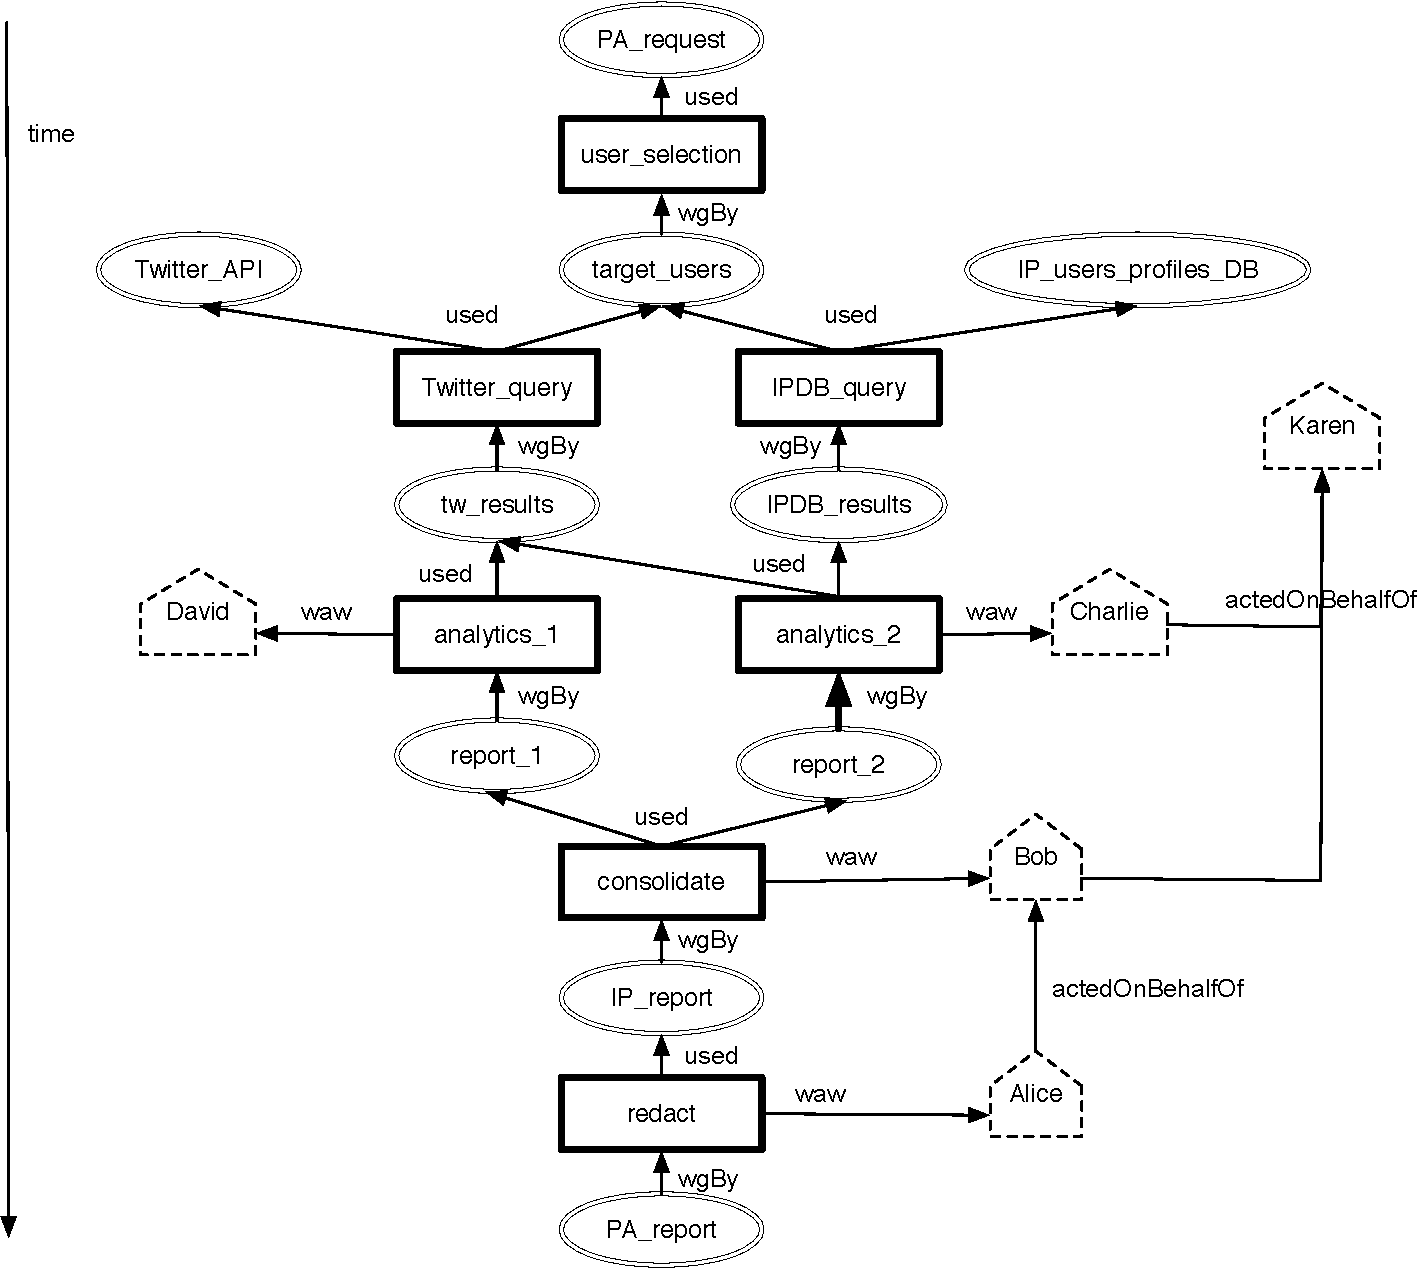
\includegraphics[width=.9\textwidth]{figures/analytics-ex-baseline-FGCS-paper}
		\caption{Example provenance graph depicting the generation of an intelligence report.}
		\label{fig:graph-example}
	\end{center}
\end{figure*}	

\paolo{
%
This provenance graph depicts a process of intelligence report generation, which is initiated by a request by PA. 
The process identifies target users from the request and acquires further information about those users, both on Twitter (\texttt{Twitter\_query}) and from a proprietary database, \texttt{IP\_users\_profile\_DB}.
%
The results are fed to two analytics sub-processes, each of which generates a report. 
%
Note that \texttt{analytics\_1} only uses Twitter data, while \texttt{analytics\_2} also uses query results of the proprietary database.
A \texttt{consolidate} step follows, which produces a master \texttt{IP\_report}.
This is checked, to validate and possibly also to remove sensitive information, before the final \texttt{PA\_report} is generated for the customer.
%
Notice that various agents are specified as being responsible for some of the steps, along with their chain of responsibility, i.e., \texttt{Alice} acts as \texttt{Bob}'s delegate, who in turn reports to \texttt{Karen}, along with \texttt{Charlie}}.


As we can see, the full-fledged provenance graph contains information about IP's internal business processes, including the use of a proprietary database, which IP may consider privileged.
It is therefore realistic to imagine that IP may want to \jwbtwo{hide} some of those elements. 
Using our selective disclosure model, IP marks the sensitive elements, in this case the \texttt{redact} activity as well as the references to the two analytics processes. Note that doing so does not require any knowledge of the graph topology, rather only of the nodes (either activities, entities, or agents) that are to be abstracted out.

\paolo{The PROV document represented in Fig.~\ref{fig:graph-example} is \textit{valid}, in the sense that it satisfies all the constraints specified as part of the PROV standard~\citep{w3c-prov-constraints}.
As we will see in the rest of the paper, replacing the three selected nodes with a single abstract node (an activity in this case) while preserving the validity  of the document, requires that all other nodes that lie on the directed paths that connect these nodes are also removed. 
In this example, the result of such abstraction operation is shown in Fig.~\ref{fig:graph-example-abs-1}.
}

	\begin{figure*}
		\begin{center}
			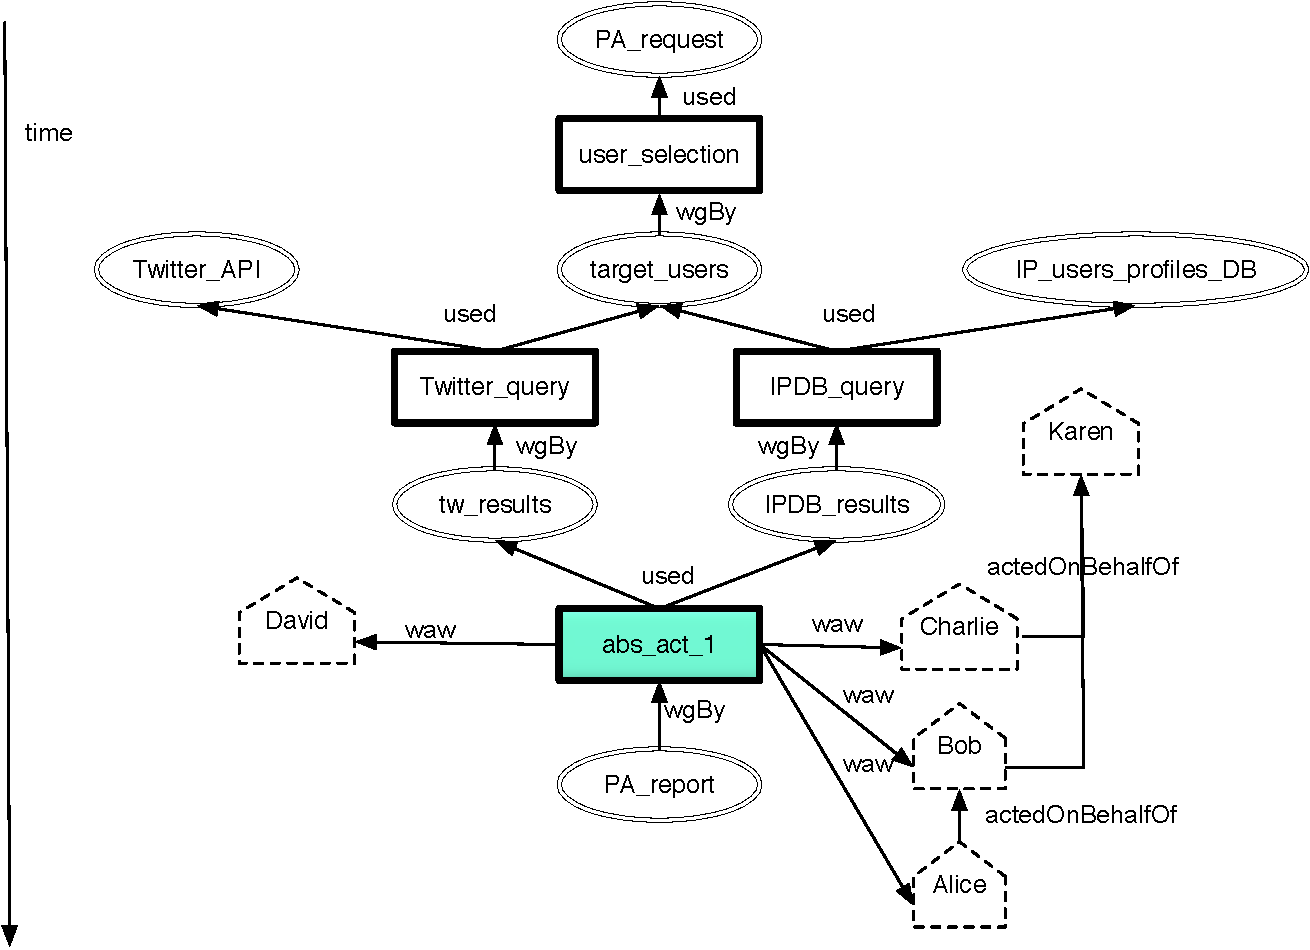
\includegraphics[width=.9\textwidth]{figures/analytics-ex-abs1-FGCS-paper}
			\caption{The result of abstracting out selected nodes \texttt{redact},  \texttt{analytics\_1}, and  \texttt{analytics\_2}  from the graph in Fig.~\ref{fig:graph-example}.} 
			\label{fig:graph-example-abs-1}
		\end{center}
	\end{figure*}	
	
\paolo{By construction, this is a new valid PROV graph. 
It is therefore possible to further abstract out some of its nodes. 
For example, IP may also decide that mentioning the use of a proprietary data source is inappropriate. 
Nodes \texttt{IP\_users\_profiles\_DB} and \texttt{IPDB\_query} are therefore abstracted out. 
As these are both entities, the new abstract node is also an entity, as shown in Fig.~\ref{fig:graph-example-abs-2}.
Note that, to PA, while still informative, the report now appears as if it had been generated from its initial request using Twitter as a data source, and without reference to specific analytics algorithms.
}

	\begin{figure*}
	\begin{center}
		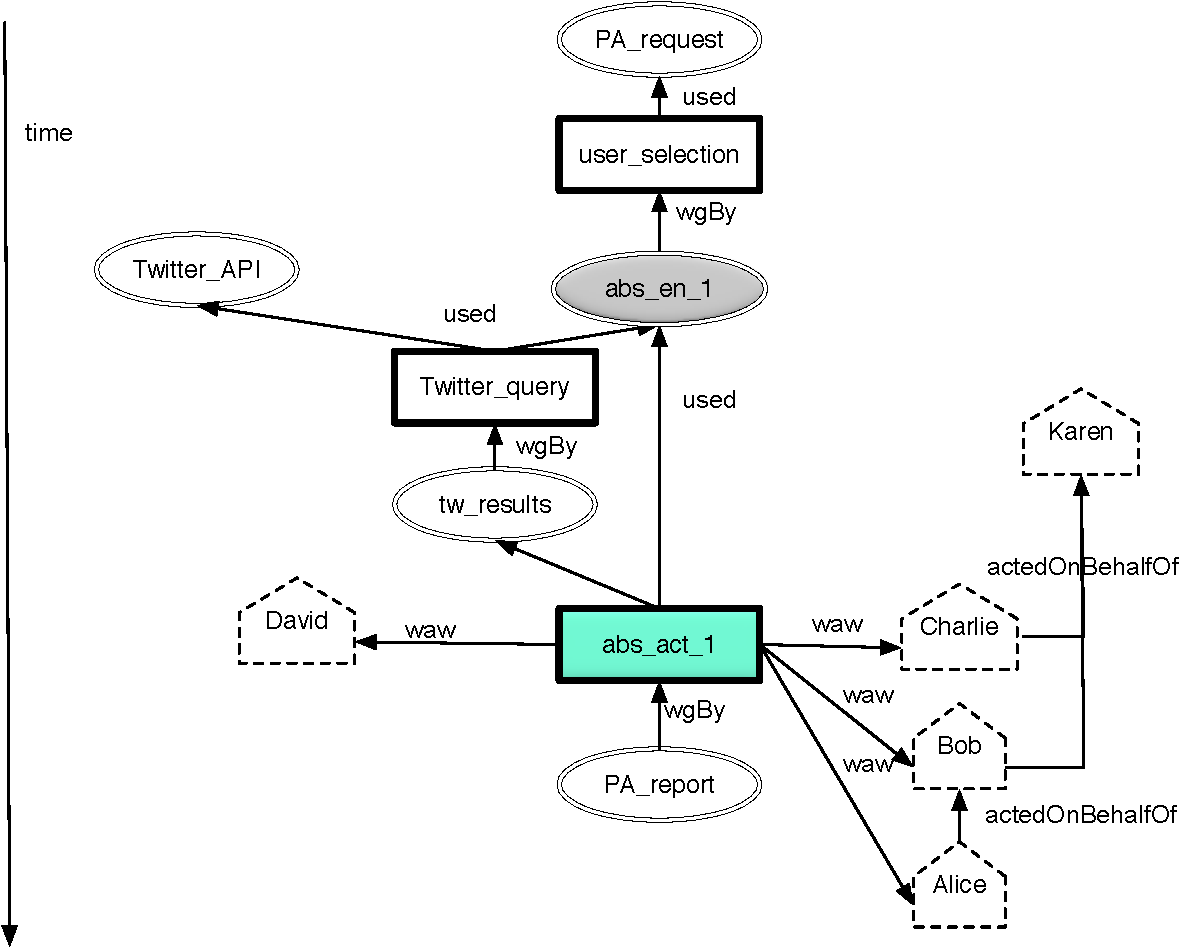
\includegraphics[width=.9\textwidth]{figures/analytics-ex-abs2-FGCS-paper}
		\caption{The result of further abstracting out \texttt{IP\_users\_profiles\_DB} and \texttt{IPDB\_query} after the first abstraction-by-gropuping step (Fig.~\ref{fig:graph-example-abs-1}).} 
		\label{fig:graph-example-abs-2}
	\end{center}
\end{figure*}	

\paolo{The mechanisms by which the data and provenance owner selects the nodes to be abstracted are not discussed in this paper, however a policy-based model is described in detail in our previous work~\citep{Missier2014}.
	Briefly, the idea, which makes use of the Bell-Lapadula model~\citep{bell1996bell},	is that the owner assigns a sensitivity value to each node, and nodes are selected to be abstracted out based on a specific  recipient's clearance level. Thus, different recipients will potentially receive different abstract versions of the same graph.
Note also that forcefully removing nodes that were not marked for abstraction has implications, too, as some of those non-sensitive nodes may have had evidential value that is now lost.
To model this problem we associate a utility value to each node, and then compute the \textit{residual utility} of the abstracted graph. 
The paper cited above~\citep{Missier2014} provides further details. 
}

We observe that removal of information from a provenance graph could be achieved in a number of other ways.
%
For example, one could simply remove the labels as well as the annotations from individual nodes and relationships, i.e., anonymize part of the graph. Doing so, however, does not hide any of the structure of the process of data production. One could further remove nodes and relationships or  indeed entire sub-graphs. The new graph will be disconnected, however, making it difficult to reconstruct the lineage of the end data product, that is, the sequence of data derivations from the initial inputs to the outcome of the process.

Instead, in our approach \jwbtwo{the selected nodes are} replaced with a new abstract node, which is then ``re-wired'' to the remaining original graph. This has the effect of hiding parts of the process structure as it was represented in the original provenance, while maintaining connectivity. One can still query the lineage, but some of the provenance elements returned by the query will now be an abstraction of the actual data production process.

The main challenge addressed in this paper is to guarantee that abstraction produces PROV-compliant  graphs,   maintaining the interoperability guarantees provided from having standardized PROV and ensuring that the results can be consumed by standard PROV tools. %We provide a proof of this in the Appendix.


\subsection{Contributions} \label{sec:contributions}

In this paper we develop a model and algorithm for performing  abstraction over PROV graphs, providing the theoretical underpinning to ensure that the abstraction process satisfies a number of properties.
%
\jwbthree{For the model development we restrict our attention almost completely to provenance graphs that contain only activities and entities, and exclude agents. The relevant relationships $\wgby$ and $\used$. The $\influence$ relation is a superproperty of both $\wgby$ and $\used$ and  we explore the advantages of incorporating it in Section~\ref{sec:influence}. 
}



%
Our main contribution is the formal \jwbtwo{functional} definition of a provenance abstraction operator ($\group$) that  rewrites  a PROV graph $\pg$ into a new graph $\pg'$, by \jwbtwo{(a)} mapping a set $V_{gr}$ of nodes (for ``vertex in a group'') in $\pg$ to a new abstract node $v_{new}$, and \jwbtwo{(b)} mapping each relationship involving elements of $V_{gr}$ \jwbtwo{(nodes)} to a new relationship involving $v_{new}$ in $\pg'$. 
The set $V_{gr}$ is chosen by the user of the abstraction operator as the set of nodes she wishes to \jwbtwo{hide, and the graph rewriting operator $\group$ is defined in three steps using three subordinate operators, detailed in Section~\ref{sec:grouping}. }


\jwbtwo{Our grouping operator ensures two} formal properties of $\pg'$: firstly, \jwbtwo{validity}: if $\pg$ is a \jwbtwo{valid} PROV graph, that is, it conforms to the PROV data model~\citep{w3c-prov-dm}, then $\pg'$ is also a \jwbtwo{valid} PROV graph.
%\jwbtwo{: if $\pg$  satisfies all PROV constraints~\citep{w3c-prov-dm}, then $\pg'$  also }~\jwbtwo{satisfies all PROV constraints}. %\jwbtwo{Together these two properties ensure  the validity of $\pg'$.}
\jwbtwo{Secondly}, no  \jwbtwo{unjustified} dependencies are introduced into $\pg'$: a  relationship involving $v_{new}$ is only created as a result of a mapping from an existing relationship involving elements of $V_{gr}$. Strictly, if $a$ and $e$ are not \textit{directly} related in $\pg$, we guarantee that they are not directly related in $\pg'$.  Note that new indirect dependencies between two nodes in $\pg'$, manifested as new paths in the graph, may be introduced, however we argue that these are always justified by the topology of the underlying graph $\pg$.

\jwbtwo{A guiding principle throughout is that of minimal damage.  We require that the grouping operator inflicts minimum unnecessary damage on the graph, while meeting the first two constraints. }
 

\jwbtwo{It is important to observe here that the task that we set ourselves is to develop this abstraction operator given an \emph{arbitrary} set of nodes in the graph that must be abstracted. 
For example, we do not allow ourselves the  luxury of partitioning the set before the $\group$ operator is applied. Here we wish to develop a pure PROV graph abstraction operator that can be applied independently of, or in combination with, other solutiions.}


Furthermore, by making the abstraction operator closed with respect to the set of valid PROV graphs, abstraction can be naturally composed, i.e., \jwbtwo{ using the $\group$ operator} one can abstract $\pg'$ into some $\pg''$ as we have shown in the earlier example.

%
Finally, note also that $\pg'$ itself has also an associated provenance graph, that is, a record of the provenance abstraction process as it was applied to $\pg$. 
PROV provides a syntactic facility to maintain the association between a provenance graph and its own provenance, namely using the ``provenance of provenance'' mechanism (i.e., bundles~\citep{w3c-prov-dm}).



%\subsection{A terminological aside.} 

%\jwbtwo{In Zoom~\citep{DBLP:conf/icde/BitonBDH08} an abstraction mechanism is a mechanism that presents the most relevant provenance information to a user. }

%\jwbtwo{Our own previous work~\citep{MBGCD14}.}

%\jwbtwo{In~citep{Moreau2015} the author discusses a variety of means of abstracting provenance graphs, including~\citep{MBGCD14}, in which the term carries the same meaning as in this work.  Also discussed are the Abstract Provenance Graphs" from~\citep{ZinnLudascher2010}. In these, abstraction is performed using static analysis of a configured workflow before the provenance is created, and a homomorphism between the abstract and the concrete graph is demonstrated. In~\citep{Cohen-Boulakiaetal2008} the authors show how the user views that they present allow provenance to be reasoned about at different levels of abstraction. }

%\jwbtwo{This understanding of abstraction, and of the ability to move between different levels of abstraction, is key to our understanding of the term here. }











%
%The remainder of the paper is structured as follows. After a review of related work, in Sec.~\ref{sec:prov-core} we introduce the fragment of the PROV model that defines the scope of our work, followed by an overview of the approach and summary of contributions (Sec.~\ref{sec:overview}).
%%
%The core technical material is in Sec.~\ref{sec:grouping}, where we define abstraction over provenance in terms of a \textit{grouping} operator, present its functional specification, and show that grouping maps a graph into a new graph that conforms to the same relational schema.


 
\section{Related Work}  \label{sec:related}

Work related to our research is broadly motivated either by the need to simplify provenance graphs to facilitate their understanding by humans, or to enforce access control over parts of the graph, or to summarise a collection of similar provenance graphs in order to reduce both space and query complexity.

\subsection{Creating views over provenance}

Work on provenance abstraction generally combines two elements, namely a technique or algorithm for graph editing, and a policy framework to drive the algorithm. As mentioned, in this paper we focus exclusively on the former, while the latter is described in a separate paper\jwb{~\citep{MBGCD14}.}
 

Work to create views over provenance graphs for the purpose of either reducing their complexity, and/or removing sensitive information, was arguably pioneered by the Zoom system~\citep{DBLP:conf/icde/BitonBDH08}. In Zoom, the main assumption is that  the graph is a trace that specifically represents the execution of a dataflow. This is a common occurrence in e-science, where workflows that follow the  dataflow model are a popular high level programming paradigm.
%
In this setting views over provenance are effectively a form of abstraction and are computed based on the user's indication of which workflow modules (tasks) are relevant, or perhaps based on which modules the user has access to. Thus, key to this approach is knowledge of the underlying workflow structure, which is used to specify the nodes in the graphs to be abstracted. This sets Zoom apart from our work, which instead investigates the properties of a grouping operator \textit{independently of the origins of the trace to which it is applied}. 

Also specific to workflow-generated provenance, and thus too narrow in scope for our purposes, is a  strand of research that investigates the problem of preserving the privacy of functions used in workflows, when a large number of input/output pairs for those functions is revealed through the provenance traces of multiple workflow executions. This work on  \textit{module privacy}~\citep{Davidson:2011:PP:1938551.1938554,Davidson2010a,Davidson:2011:PVM:1989284.1989305} is concerned with protecting the semantics of workflow modules. 
It applies anonymization techniques specifically to provenance graphs and is again centred around a workflow-specific form of provenance and  is thus also peripheral to our interest.

% that contain traces of dataflow execution (a ``run''). . This is similar to our work in two ways. Firstly, a view is an answer to a provenance query, which accounts for users preferences and privileges. While provenance sharing policies are not a part of the model and thus are not mentioned explicitly, it is easy to imagine our policies providing input to the view generator.
%Secondly, Zoom too has a notion of consistency, i.e., views must be valid provenance graphs. The main difference with our work is that in Zoom, provenance views are really a by-product of user views over the workflow whose execution the provenance graph represents, whereas our approach is based on a ``PROV-lite'' provenance model that makes no assumptions on the structure of the process that generates the graph.
%

Closer to our abstraction model, both in motivation and in its technical approach, is the ProPub system~\citep{springerlink:10.1007/978-3-642-22351-8_13}, which computes views over provenance graphs that are suitable for publication by meeting  certain privacy requirements. In ProPub, users specify edit operations on a graph, such as anonymizing, abstracting, and hiding certain parts of it.
% (here the term ``abstracting'' is interpreted as ``zooming out'', much as in~\citep{DBLP:conf/icde/BitonBDH08} mentioned above).
%
The operations are specified as logic rules, and are interpreted natively by the Datalog-based prototype implementation. ProPub adopts an ``apply--detect--repair'' approach, whereby user rules are applied to the graph first, then consistency violations that may occur in the resulting new graph are detected, and a final set of edits are applied to the graph in order to repair such violations. In some cases, this causes nodes that the user wanted removed to be reintroduced, and it is not always possible to satisfy all rules. 
%
In contrast, our grouping involves more simply a set of nodes to be abstracted (but note that anonymization is a particular case, when the group contains a single element). In return for this simplicity in the specification of the nodes to be grouped, our method always produces a valid abstract graph while ensuring that the nodes specified in the policy are removed. 
%, as described in detail in the next section. In order to further clarify the relationship between the two approaches, in Appendix~\ref{sec:appendix} we show how our algorithm computes an abstraction over the same example graph used in the ProPub paper.

Finally, \textit{provenance redaction}~\citep{Cadenhead:2011:TPU:1998441.1998456} employs a graph grammar technique to edit provenance that is expressed using the Open Provenance Model~\citep{Moreau2010a} (a precursor to PROV), as well as a redaction policy language.
%
Although the authors claim that the redaction operators ensure that specific relationships are preserved, this critical issue is not addressed formally in the paper, i.e., with reference to the OPM semantics.
%
In contrast, the formal schema and set of constraints that come with PROV~\citep{w3c-prov-dm,w3c-prov-constraints} provide the necessary grounding for reasoning about the validity-preservation properties of the editing operations.
%Cadenhead, Tyrone, Vaibhav Khadilkar, Murat Kantarcioglu, and Bhavani Thuraisingham. “Transforming Provenance Using Redaction.” In Proceedings of the 16th ACM Symposium on Access Control Models and Technologies, 93–102. New York, NY, USA: ACM, 2011. doi:10.1145/1998441.1998456.

\subsection{Provenance Access Control}

Most of the work on protecting access to sensitive provenance includes policy models that extend traditional data access control frameworks (RBAC), with a distinction made between PBAC (Provenance-Based Access Control) and PAC (Provenance Access Control).
%
PBAC is about policy to specify access rights to data objects based on their provenance.
%
An example, from~\citep{nguyen2012dependency}, is a rule of the form ``only the student submitter can access the graded homework object''. 
%
This rule can be enforced by looking for a dependency path in a provenance graph, whereby a given homework is attributed to a specific student (i.e., relation \textit{IsAuthoredBy} in the Open Provenance Model). This assumes that the object's attribution is explicit in the provenance graph. It is less clear how such a rule would be evaluated when the provenance is incomplete with respect to such attribution dependency, however.

PAC, or how to enforce access control on parts of a provenance graph, is more directly relevant to our work. An analysis of some of the  challenges associated with secure provenance exchange can be found in  \citep{Braun:2008:SP:1496671.1496675}, where 
%[2] U. Braun, A. Shinnar, and M. Seltzer. Secure provenance. In The 3rd USENIX Workshop on Hot Topics in Sec., pages 1–5, Berkeley, CA, USA, 2008.
examples are presented that show how the provenance of data can be more sensitive than the data itself.
%
Another position paper \citep{Hasan:2007:ISP:1314313.1314318}
% [9] R. Hasan, R. Sion, and M. Winslett. Introducing secure provenance: problems and challenges. StorageSS ’07, pages 13–18, 2007.
describes the challenges associated with the exchange of provenance across multiple partners, in a setting where forgery of provenance by malicious users is a possibility, and where users may collude to reveal sensitive provenance to others. These are all common and complex security problems. Unfortunately, the paper stops short of providing any hints at technical solutions, and indeed it is not clear how these problems are specific to provenance, as opposed to data sharing in general.

A concrete specification of an access control system or provenance~\citep{Cadenhead:2011:LPA:1943513.1943532} consists of a XACML-based policy language, in which path queries are used to specify target elements of the graph, as well as an implementation architecture and a prototype.
%Cadenhead, Tyrone, Vaibhav Khadilkar, Murat Kantarcioglu, and Bhavani Thuraisingham. “A Language for Provenance Access Control.” In Proceedings of the First ACM Conference on Data and Application Security and Privacy, 133–144. New York, NY, USA: ACM, 2011. doi:10.1145/1943513.1943532.
%
%\item \citep{Sun:2013:EAC:2435349.2435390}
%Sun, Lianshan, Jaehong Park, and Ravi Sandhu. “Engineering Access Control Policies for Provenance-aware Systems.” In Proceedings of the Third ACM Conference on Data and Application Security and Privacy, 285–292. New York, NY, USA: ACM, 2013. doi:10.1145/2435349.2435390.


%\mnote{Cite as reference: \citep{Altintas2010a}}

\subsection{Summarisation of provenance graphs}

A loosely related strand of research in this area aims at summarising a collection of provenance graphs by constructing a ``super-graph'' that captures the common features across a collection of similar graphs, such as those that are produced by repeating execution of a process with different inputs and parameters. This has been addressed with an aim to improve provenance queries \citep{DBLP:journals/jidm/El-JaickML14}, as well as to provide a compact but approximate representation of provenance at the possible cost of information loss \citep{Ainy:2015:ASD:2806416.2806429}. This work is only peripherally relevant here, as our approach only operates on one graph at a time. 

\paolo{In \citep{moreau2015aggregation} a mechanism is proposed to automatically construct aggregations from a single PROV graph.
This relies on the concept of \textit{provenance types}, which are fixed-length paths in the graph that occur more than once. 
The aggregation is defined as a mapping from provenance nodes to the provenance types, and there is a way to connect these types into a new PROV-like graph, by similarly mapping the graph edges to new weighted edges.
The result is a new graph that is meant to capture the ``essence'' of a fine-grained set of provenance  statements by observing regularities in the original graph.
This is substantially different from our approach, namely (i) the choice of nodes to aggregate is driven by the discovery of provenance types, which is entirely driven by graph topology and not by a user choice, and (ii) there is no intent to generate \textit{valid} PROV graphs, which is instead the main goal of our transformation.  
Thus, the approach is not suitable to support policy-driven (or other user-oriented) selective disclosure, and the aggregation operation produces a graph that may violate PROV constraints.
}

\subsection{General graph anonymization}

For completeness, we briefly mention more general techniques for graph editing, largely motivated by the need to preserve privacy in social network data. This body of work, which is not specific to provenance, extends the well-known data anynomization framework developed for relational data to graph data structures~\citep{springerlink:10.1007/978-3-540-78478-4_9,Bhagat:2009:CGA:1687627.1687714,Liu:2008:TIA:1376616.1376629}. The main idea is to randomly remove arcs between two nodes and replace them with new ones. As arcs in PROV graphs represent relationships with a given semantics, this approach generally results in false dependencies being created in the edited graph, and is therefore not viable. 
%
The main value of this body of work in this setting, as summarised in~\citep{Zhou:2008:BSA:1540276.1540279}, is to ensure that various forms of anonymization are provably robust to attacks from adversaries who can potentially leverage their partial information about fragments of the graph, to infer additional knowledge. In this paper we do not discuss the robustness of abstraction by grouping, indeed we do not consider any specific threats, and so the challenge of preventing the reconstruction of the abstracted fragments of provenance graphs is left for future work.
%\citep{Bhagat:2009:CGA:1687627.1687714}  // anon social network graphs -- shrivastava

%\citep{Liu:2008:TIA:1376616.1376629}  // Towards identity anonymization on graphs

%\citep{Zhou:2008:BSA:1540276.1540279}  // survey of anon graph data for social network applications



%%%%%%%%%%%%
%%
%%%%%%%%%%%%

\section{Background}
\label{sec:prov-background}

\subsection{Core PROV model} \label{sec:prov-core}

We now introduce the core elements of the PROV model, which forms the basis for the grouping operator.
%
We maintain a dual view of provenance, both as a relational model (with binary relations) and as a graph model. Viewed as a relational model, PROV includes three types of elements: Entities ($\en$), Activities ($\act$), and Agents ($\ag$), and several types of relations amongst them. 
In line with the description in~\citep{w3c-prov-dm} (Section 2), PROV is defined by the following core relations, with common abbreviations in brackets. 

\begin{eqnarray*}
Used~~(\used)  & \subseteq & \act \times \en \\
WasGeneratedBy~~(\wgby) & \subseteq  & \en \times \act \\
WasDerivedFrom~~(\wdf) & \subseteq   & \en \times \en \\
WasInvalidatedBy~~(\inv) &  \subseteq &  \en \times \act \\
WasAssociatedWith~~(\waw) & \subseteq & \act \times \ag \\
ActedOnBehalfOg~~(\delegate) & \subseteq & \ag \times \ag \\ 
WasAttributedTo~~(\attrTo) & \subseteq & \en \times \ag \\
WasInformedBy~~(\wasInfBy) & \subseteq & \act \times \act
\end{eqnarray*}


\begin{figure}
\centering
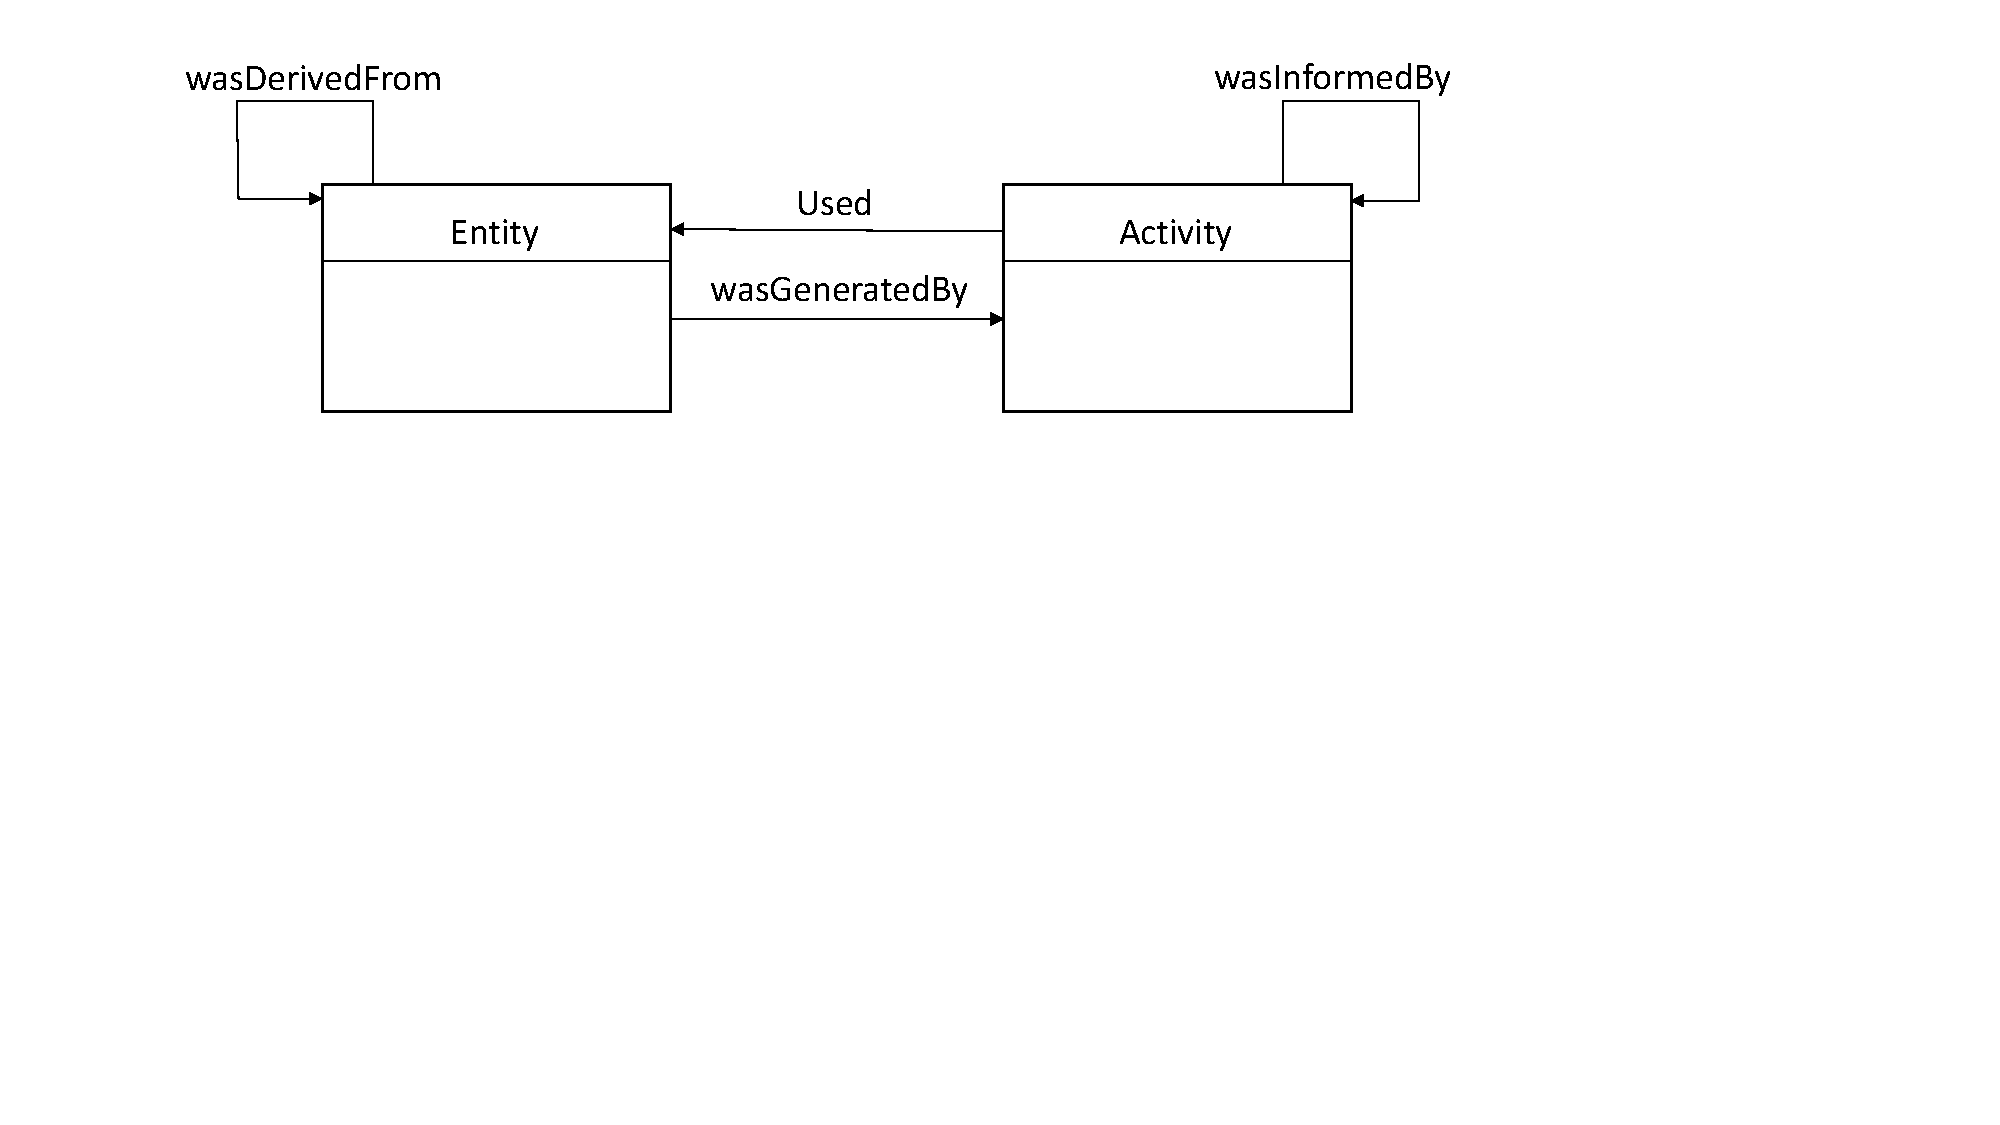
\includegraphics[scale=.45]{figures/prov-essentials.pdf} 
\caption{Core elements of the PROV model, adapted from~\citep{w3c-prov-dm}}
\label{fig:prov-core}
\end{figure}

%\subsection{Bipartite PROV: $\guEA$}  \label{sec:prov-guea}
These are summarized in Fig.~\ref{fig:prov-core}.
%

\jwbtwo{In this paper} we are going to restrict ourselves to an even simpler model, consisting only of $\en$, $\act$, and relations $\used$ and $\wgby$.
% Agents and the relations that involve them are introduced in Sec.~\ref{sec:agents-abstraction}.
%
Further extensions to the additional relations --- $\wdf$ and $\wasInfBy$ --- are straightforward and are not considered in detail.

%
An instance  of the model is a provenance document $D$, consisting of sets $en \in \en$ and $act \in \act$ of symbols, and sets of relation instances $\{ \wgby(e,a)  | e \in \en, a \in \act \} \cup   \{ \used(a,e)  | e \in \en, a \in \act\}$. 

%
As these relations are binary, we view $D$ as a digraph $G=(V,E)$, where $V= \en \cup \act$, and each relation instance maps to a labelled directed edge. By convention, we orient these edges from right to left, to denote that the relation ``points back to the past''. Thus:
$a \xleftarrow{\wgby} e \in E$ iff $\wgby(e,a) \in D$, and $e \xleftarrow{\used} a \in E$ iff $\used(a,e) \in D$.
%
We denote the label associated to edge $(v_i, v_j)$ as $\elabel(v_i,v_j)$. 

%
Note that, by definition of the relations, $G$ is a bipartite graph.
We denote the set of all such graphs by $\guEA$, to indicate that they only contain $\en$ and $\act$ nodes, and $\wgby$ and $\used$ edges.
Fig.~\ref{fig:baseline-ug-ae} portrays a simple $\guEA$ graph that we will be using as a running example. %\comment{This sentence isn't true. Fig 5 isn't the same as fig 6. Fig 6 = Fig 7,  but then Fig 8 = Fig 5. }

 %In Sec.~\ref{sec:agents-abstraction} we are going to extend this set to include agents as well as additional relations.

%\comment{Old version is above, new below}

\begin{figure}
\centering
%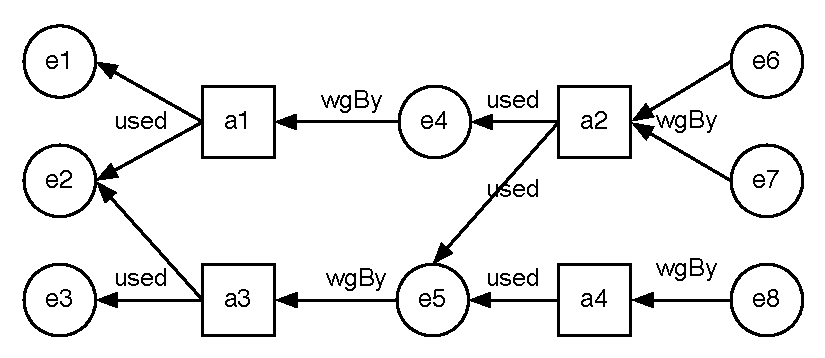
\includegraphics[scale=.6]{figures/baseline-ug-ae.pdf} 
%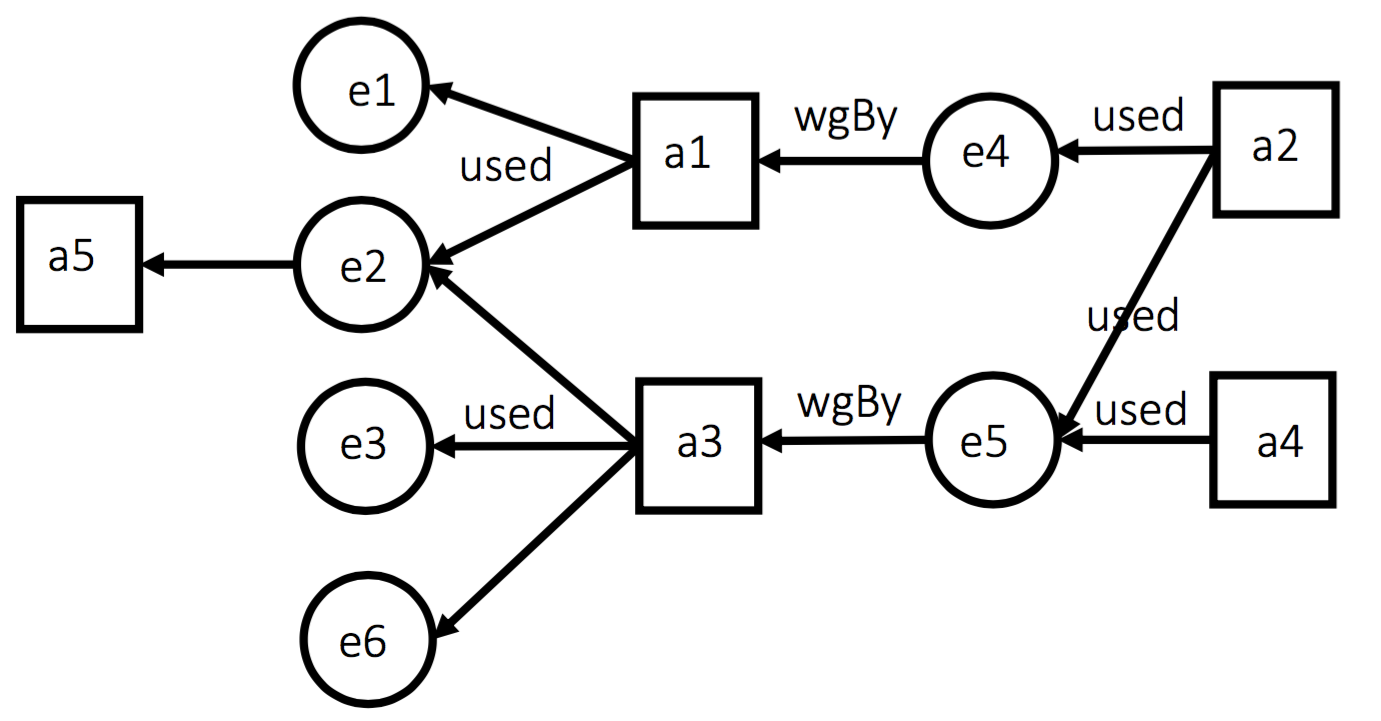
\includegraphics[scale=.15]{reworked-fig5.png} 
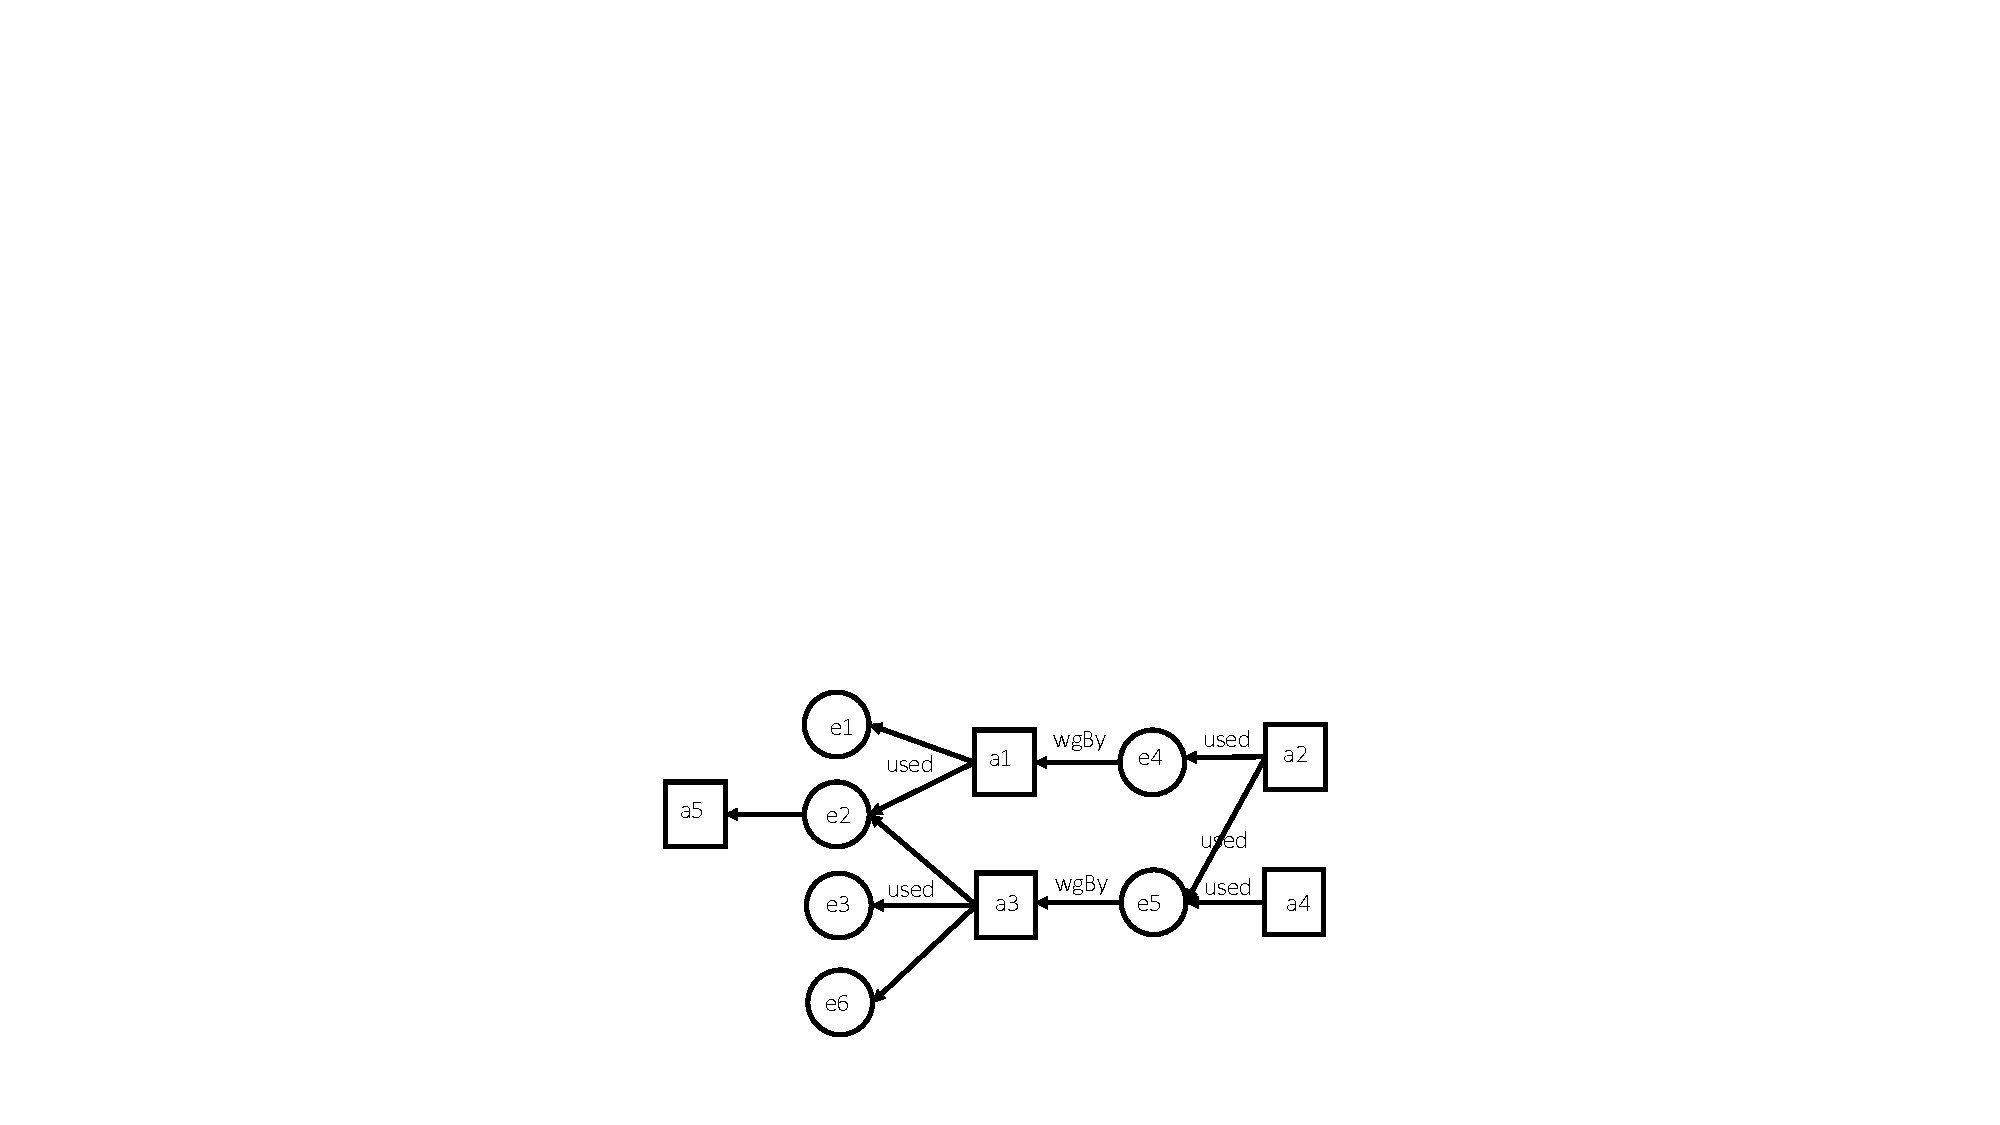
\includegraphics[scale=.6]{reworked-fig5.pdf} 
\caption{$\guEA$ provenance graph used as a running example to illustrate abstraction by grouping.}  \label{fig:baseline-ug-ae}
\end{figure}

\subsection{Events in $\guEA$}  \label{sec:prov-events}

\label{sec:events}

Central to PROV is the notion that provenance is marked by events. A partial order is defined over events, so that it may or may not be possible to establish whether or not one event precedes another. 
%
Events occur instantaneously, and they mark the lifetime boundaries of Entities (generation, invalidation), Activities (start, end), and Agents (start, end), as well as some of the interactions amongst those elements. These include the generation and usage of an entity by an activity, attribution of an entity to an agent, and more. More specifically, the PROV-CONSTRAINTS document~\citep{w3c-prov-constraints} defines the following types of events (quoted verbatim from Section 2.2):

\begin{itemize} %
	\item\textbf{An activity start event} is the instantaneous event that marks the instant an activity starts.
	
	\item\textbf{An activity end event} is the instantaneous event that marks the instant an activity ends.
	
	\item\textbf{An entity generation event} is the instantaneous event that marks the final instant of an entity's creation timespan, after which it is available for use. The entity did not exist before this event.
	
	\item\textbf{An entity usage event}  is the instantaneous event that marks the first instant of an entity's consumption timespan by an activity. The described usage had not started before this instant, although the activity could potentially have used the same entity at a different time.
	
	\item\textbf{An entity invalidation event} is the instantaneous event that marks the initial instant of the destruction, invalidation, or cessation of an entity, after which the entity is no longer available for use. The entity no longer exists after this event.
	
\end{itemize}
%\end{description}

We formally express events by introducing a set $\Ev$ of event symbols, with a pre-order\footnote{Recall that a pre-order is a binary relation with reflexivity and transitivity, but no symmetry or anti-symmetry.} $\preorder ~~\subset \Ev \times \Ev$, and the following set of partial functions that associate events to elements and relations in a provenance instance:
\begin{align*}
start: \act \rightarrow \Ev \\
end: \act \rightarrow \Ev \\
ev: \wgby \cup \used \cup \inv \rightarrow \Ev
\end{align*}	
As an example, in the graph of Fig.~\ref{fig:baseline-ug-ae} the generation relation $\wgby(e_4, a_1)$ has an associated generation event $ev(\wgby(e_4, a_1))$, whilst $a_1$ has start and / or end events, written $start(a_1)$ and $end(a_1)$, respectively. Similarly, usage of $e_4$ by $a_2$ is marked by event $ev(\used(a_2, e_4))$. Finally, if $e_4$ had been invalidated by some $a$ (not in the figure), this would be represented by an invalidation event $ev(\inv(e_4,a))$.

Temporal constraints involving events, and expressed by means of their pre-order relation $\preorder$, play a key role in the definition of \textit{valid} provenance instances, as described next.

\subsection{Constraints and valid $\guEA$ graphs}
\label{sec:prov-constraints}

%As mentioned earlier, our goal in this work is to define transformations of a valid PROV instance into new valid instance, whilst providing obfuscation by abstracting out some of its details. 
Validity of a PROV document is defined in terms of a set of constraints, as stated in the PROV-CONSTRAINTS document~\citep{w3c-prov-constraints}.
%
For instance, Constraint 55 states that the Entities and Activities are disjoint:  $\en \cap \act = \emptyset$.
Thus, a document $D$ that contains both statements (1) $a_1 \used~e_1$ and (2) $e_1 \used ~a_1$ cannot be valid, because by definition% of $\used$ given earlier,
 (1) entails  $e_1 \in \en$, $a_1 \in \act$, while (2) entails $a_1 \in \en$, $e_1 \in \act$, violating the constraint.
%
Note that disjointness constraint 55 entails that $\guEA$ graphs are bipartite.

In this paper we are mainly concerned with temporal constraints, which apply to $\guEA$ instances and determine the admissible partial ordering of the event types introduced in the previous section.
With reference to a graph $\pg$, these are (including constraint (55) above, and using the original numbering in~\citep{w3c-prov-constraints})

\begin{itemize}
	
	\item\textbf{C1: entity-activity-disjoint (Constraint 55):} \[\en \cap \act = \emptyset\]
	
	\item\textbf{C2: generation-generation-ordering (Constraint 39):}  If an entity is generated by more than one activity, then the generation events must all be simultaneous.
	
	Let 
	$gen_1 = ev(\wgby(e, a_1))$, $gen_2 = ev(\wgby(e, a_2)) \in \pg$. Then  \[gen_1  \preorder  gen_2, \quad gen_2 \preorder gen_1\] must hold.
	
	\item\textbf{C3: generation-precedes-usage(Constraint 37):} A generation event for an entity must precede any usage event for that entity.
	%
	For any $a \in \act$ such that $\used(a,e) \in \pg$, \[	ev(\wgby(e, a)) \preorder ev(\used(a,e))\] must hold.
	
	\item\textbf{C4: generation-precedes-invalidation (Constraint 36):} The generation event (or, more accurately, the set of simultaneous generation events) for an entity must precede the invalidation event.
	
	For any $a,a' \in \act$ such that $\wgby(e, a))$, $\inv(e,a') \in \pg$ :
	\[ ev(\wgby(e, a)) \preorder ev(\inv(e,a')) \]
	
	\item\textbf{C5: usage-precedes-invalidation (Constraint 38):} Any usage event for an entity must precede the invalidation event.
%	
	For any $a,a' \in \act$ such that $\used(a,e))$, $\inv(e,a') \in \pg$ :
	\[ ev(\used(a,e)) \preorder ev(\inv(e,a')) \]
	
	\item\textbf{C6: usage-within-activity (Constraint 33):} Any usage of $e$ by $a$ cannot precede the start of $a$ and must precede the end of $a$. For any $e\in \en, a \in \act$ such that $\used(a,e) \in \pg$:
	\[start(a) \preorder ev(\used(a,e))   \preorder end(a)\]
	
	\item\textbf{C7: generation-within-activity (Constraint 34):} The generation of $e$ by $a$ cannot precede the start of $a$ and must precede the end of $a$.
	Let $\wgby(e,a) \in \pg$:
	\[ start(a) \preorder ev(\wgby(e,a))  \preorder end(a)\]
	
	\item\textbf{C8: invalidation-invalidation-ordering (Constraint 40):}	If an entity is invalidated by more than one activity, the events must all be simultaneous. \jwbtwo{If $\inv(e,a_1), \inv(e,a_2) \in \pg$, then }
	  \begin{align*}
          &\jwbtwo{ev(\inv(e,a_1)) \preorder  ev(\inv(e,a_2)) ~~\mathrm{and}} \\
          &\jwbtwo{ev(\inv(e,a_2)) \preorder  ev(\inv(e,a_1))}
          \end{align*}
\jwbtwo{must hold.}

\end{itemize}

Additional relevant constraints state that multiple start (resp. end, invalidation) events must all be simultaneous, and that the start event of an activity must precede the end event for that activity.
\\

\begin{definition}[Validity]
 A graph $G \in \guEA$ is valid iff it satisfies constraints C1-C8.
	\label{def:valid-guea}
\end{definition}

%\comment{should finish off with a sign-post para here}
\jwb{In the next section, we present the main result of this work, the $\group$ operator. We will return to the constraints above in Section~\ref{sec:event}, where we demonstrate that application of the group operator maintains the validity of the above constraints, in a manner which we will clarify further in Section~\ref{sec:event}.  
}


\section{Grouping Provenance graph nodes}  \label{sec:grouping}

%\comment{discuss (somewhere) implications of relaxing the assumption about connectivity in Section~\ref{sec:closure}.}

%\comment{fix next two paras.} 
%
%\comment{need to be clear (again) about assumptions. We have motivated these in Sec~\ref{sec:motivating}. } 

As mentioned in Sec.~\ref{sec:contributions}, our goal is to define \jwbtwo{a} graph editing operator that selectively removes information from a graph $G \in \guEA$, yielding a new graph $G' \in \guEA$. \jwbtwo{We require the final operator to remove all the chosen nodes, and replace them by a single abstract node.} \jwbtwo{As discussed in Section~\ref{sec:motivating}, this may be to avoid inadvertently revealing any internal business processes or details about the chain of command.}

\jwbtwo{Furthermore, we wish the modified graph to be a valid PROV graph, in the sense that the relations and constraints from Section~\ref{sec:prov-background} are respected. This will allow the output to be consumed by any system capable of reading the PROV language.}

%
%\jwbtwo{It is important to note, however, that} simply reconnecting the remaining nodes generally may lead to an invalid graph. 
%
%A simple example is a graph defined by: $\{\used(a, e_1)$, $\wgby(e_2, a) \}$ where activity $a$ is removed. This results in two disconnected nodes $e_1$, $e_2$, with no indication of the connection between them. % because no relationship can be inferred between them from the original graph.

\jwbtwo{In this section, we focus exclusively on the definition of the} $\group$ graph transformation operator as the prime way to achieve abstraction over provenance graphs.
%
%\jwbtwo{Let $V$ and $E$ be as defined in Section~\ref{prov-core}. }

$\group$ takes a graph $G \in \guEA$ \jwbtwo{with nodes $V$ and edges $E$} and a subset $V_{gr} \subset V$ of its nodes \jwb{that the user wishes to hide} and produces a modified graph $G' \in \guEA$. The nodes in $V_{gr}$ are ``grouped'' together and replaced by a new single node. \jwbtwo{The $\group$ operator has the following signature, where $\power(V)$ is the powerset of the nodes $V$ of the graph $G$ :}
  

\begin{equation}
Group : PG_{gu/ea} \times \power(V)  \rightarrow PG_{gu/ea} 
\end{equation}
%Here we define $\group$ over $\guEA$ graphs. This will be extended to abstraction over Agents in Sec.~\ref{sec:agents-abstraction}.


As the operator is closed under composition, further abstraction can be achieved by repeated grouping, either on multiple disjoint sets $V_{gr}$, or on sets that include abstract nodes (abstraction of abstraction).


\jwbtwo{We take a functional approach to the definition of $group$, by defining three subordinate functions and then defining $\group$ as the functional composition of these subordinate functions. }

\jwbtwo{In Section~\ref{sec:closure} we make the simplifying assumption that the set of nodes to be removed are all of the same type (either all $\en$ or all $\act$). We refer to this as \emph{homogeneous grouping} and the replacement node is imlicitly of the same type as the nodes selected to be removed.}
\jwbtwo{In Section~\ref{sec:generalisation} we remove this assumption, so the group of nodes initially selected to be removed can contain both entities and activities. A consequence of this is that the type of the replacement node is no longer implicit, and  must be  explicitly given. This leads to two variants of the operator,  depending on which type ($\en$ or $\act$) is chosen for the final replacement node.  In Section~\ref{sec:generalisation} we also identify an issue arising from simultaneous generation, and show how it may be circumvented, leading to a further varient of $\group$.  }

\jwbtwo{In Section~\ref{sec:justifying} we show that the relations in the abstract graph produced by any of the $\group$ operators are \emph{justified} by the original graph, and in Section~\ref{sec:complexity} we discuss the issue of the complexity of the operator.
}

%
%To get a quick intuition of the  problems faced in the definition of the grouping operator, consider the transformation in Fig.~\ref{fig:non-convex-ex-1}, where nodes $V_{gr} = \{e_1, e_3, e_4, e_5\}$ are simply replaced with new node $e'$ in the example graph of Fig.~\ref{fig:baseline-ug-ae}, and all edges in and out of nodes in $V_{gr}$ are just ``rewired'' in and out of $e'$. 

%\begin{figure*}
%\centering
%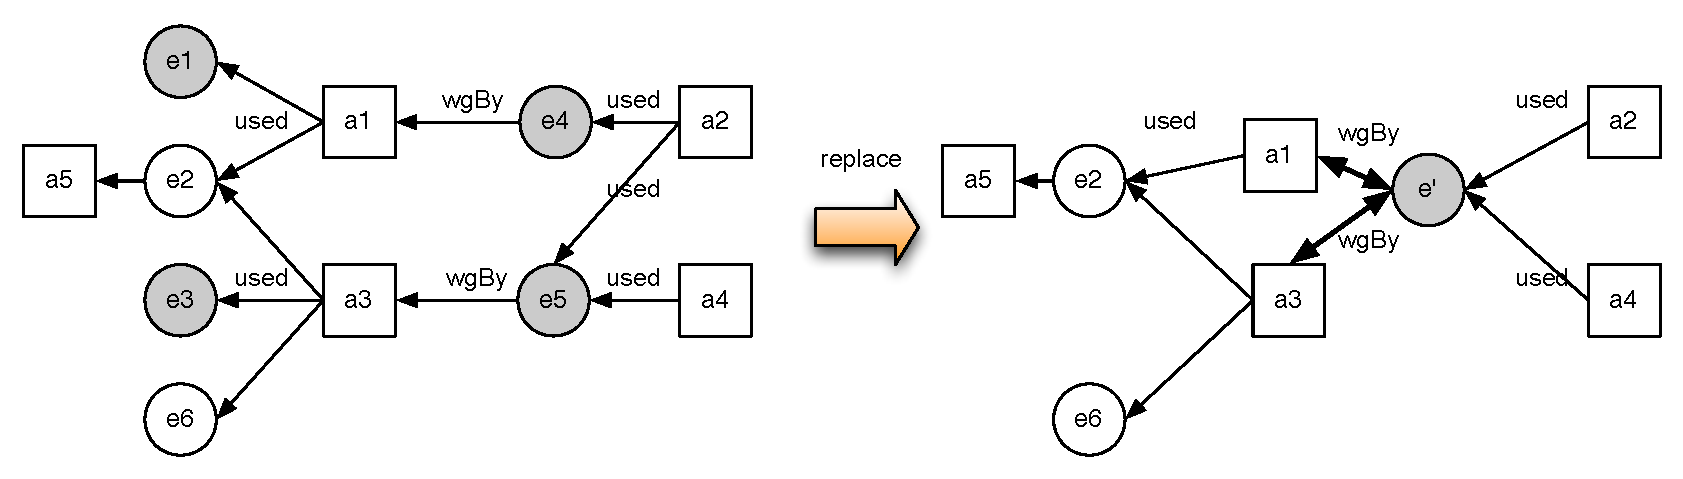
\includegraphics[scale=.5]{figures/non-convex-ex-1.pdf} 
%\caption{Example: the careless abstraction of a set of nodes may lead to a non-$\guEA$ graph.} \label{fig:non-convex-ex-1}
%\end{figure*}


\subsection{Closure and homogeneous grouping}
\label{sec:closure}

%\comment{fix below wrt text above}

\jwbtwo{In this subsection we present the homogeneous version of the $\group$ operator that will replace a selected set of nodes with an abstracted one, working under the simplifying assumption that all the nodes selected to be removed are of the same type.  As stated previously, we also wish to ensure that the final abstracted graph is a valid PROV graph.}

 \jwbtwo{Let the set of nodes to be replaced in a graph $G$ be $V_{gr}$. An issue, pointed out in the description of the ProPub system~\citep{springerlink:10.1007/978-3-642-22351-8_13}, mentioned earlier, is that removing $V_{gr}$ and replacing it with a single node can lead to cycles in the modified graph. Intuitively, this occurs when $V_{gr}$ is not``convex'', that is, there are paths in the graph that lead out of $V_{gr}$ and then back in again.}

This suggests the introduction of a preliminary closure operation \textit{pclos}(), which ensures acyclicity by capturing \jwbtwo{and including all the nodes on paths between nodes in the initial group}. It is defined as follows.

%%%%
%% closure
%%%%
\vspace*{10pt}
\begin{definition}[Path Closure]
\label{def:clos}
Let $G = (V,E) \in \guEA$ be a provenance graph, and let $V_{gr} \subset V$.  
For each pair  $v_i, v_j \in V_{gr}$ such that there \jwbtwo{are} one or more directed paths $v_i \leadsto v_j$ in $G$, let $V_{ij} \subset V$ be the set of all nodes in \jwb{all paths $v_i \leadsto v_j$}.
The Path Closure of $V_{gr}$ in $G$ is
\[\clos(V_{gr}, \jwb{G})  =  \bigcup_{v_i, v_j \in V_{gr}} V_{ij} \]
\end{definition}


\jwbtwo{Fig.~\ref{fig:convex-ex-1} illustrates $\pclos()$ in the transition from Fig.~\ref{fig:convex-ex-1}(a) to Fig.~\ref{fig:convex-ex-1}(b).  $\pclos()$ is performed on the set $\{e_1, e_3, e_4, e_5\},G)$, resulting in the set $\{e_1, e_3, e_4, e_5, a_1, a_3\}$ in Fig.~\ref{fig:convex-ex-1}(b).
}
\jwbtwo{We assume, for the moment, that nodes in $\clos(V_{gr}, G)$ induce a single connected subgraph under $G$.}
%\comment{I don't think we need the extra assumption that each source in the induced graph is connected to at least one of the sinks in the induced graph.} 

\begin{figure*}
\centering
%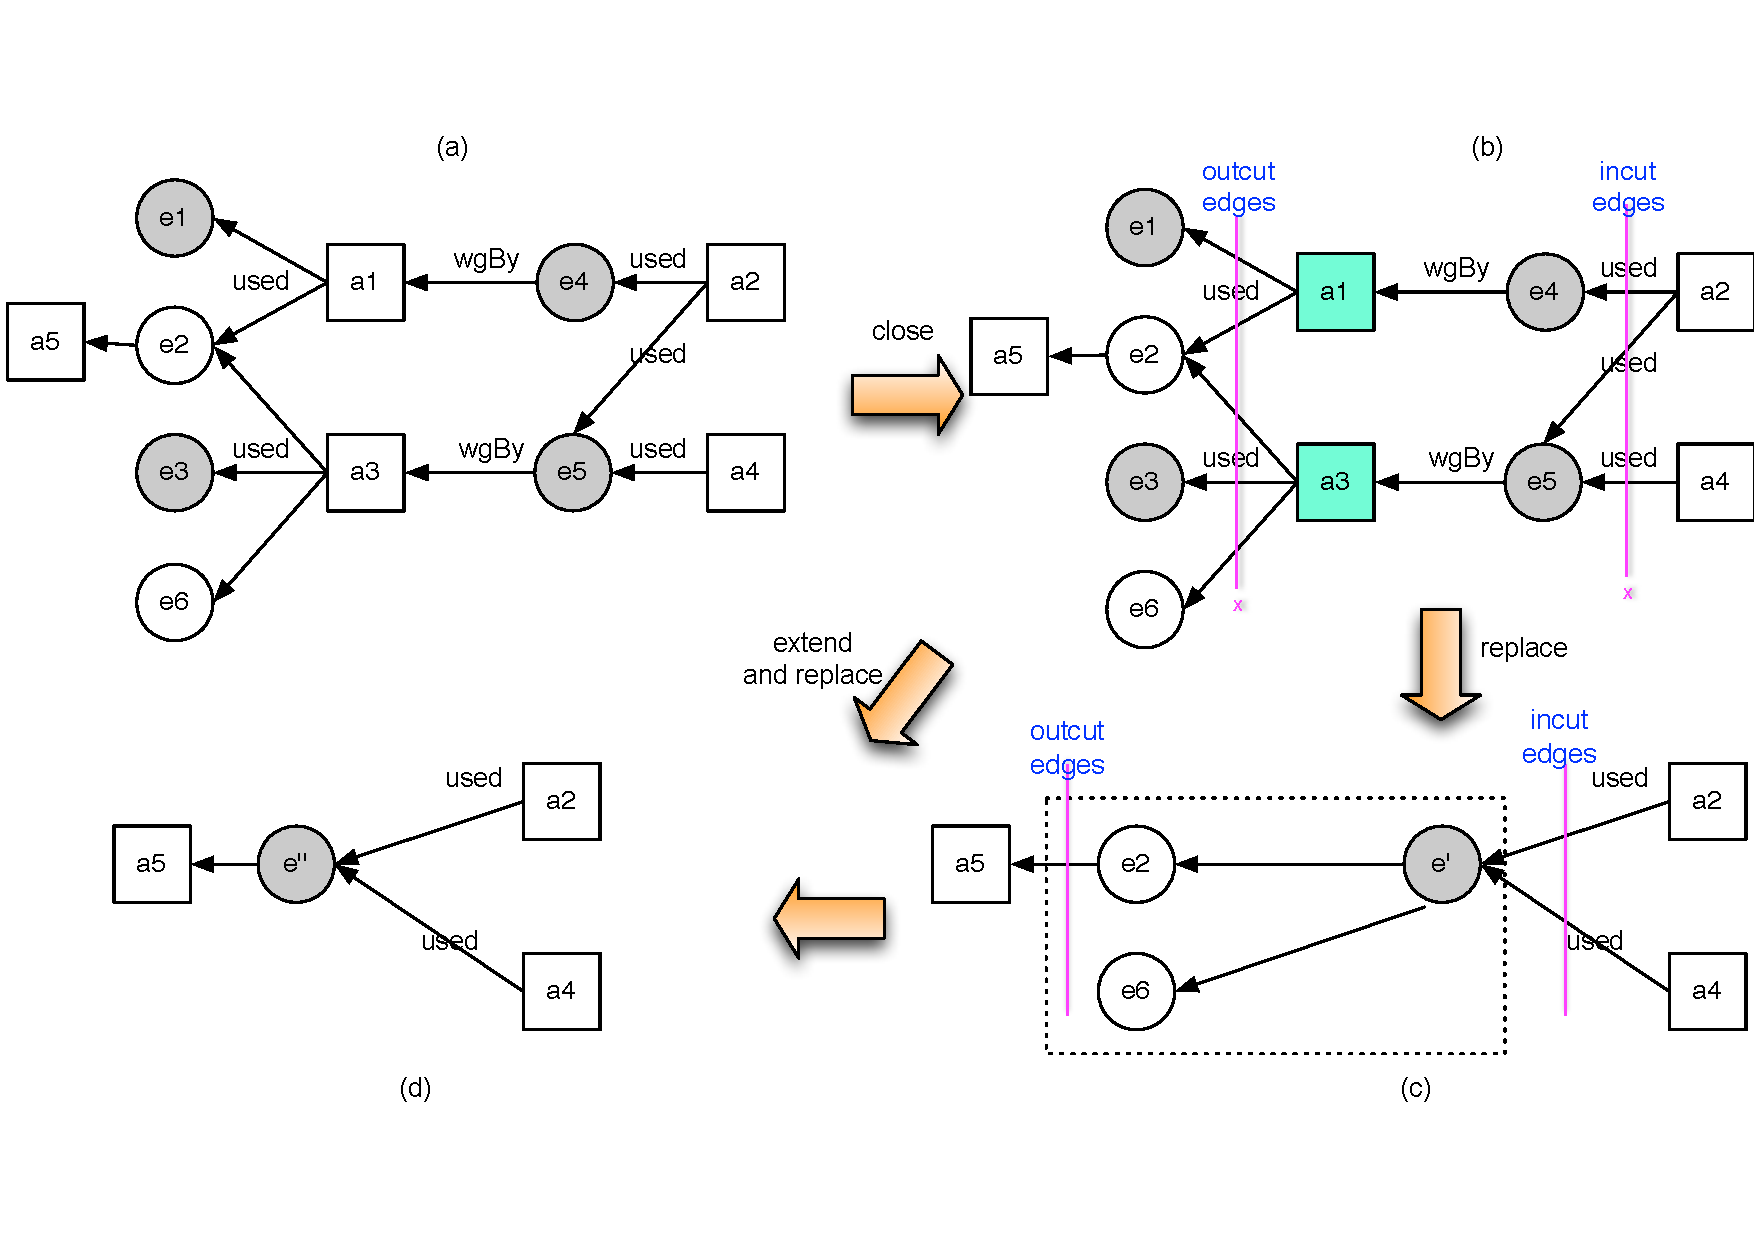
\includegraphics[scale=.5]{figures/convex-ex-1-revision.pdf} 
%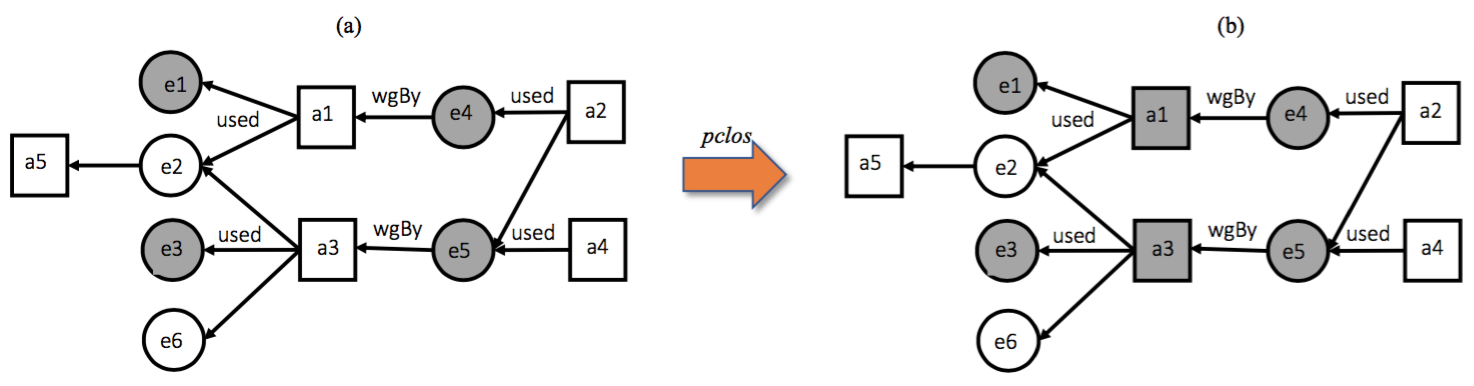
\includegraphics[scale=.27]{reworked-fig7.png} 
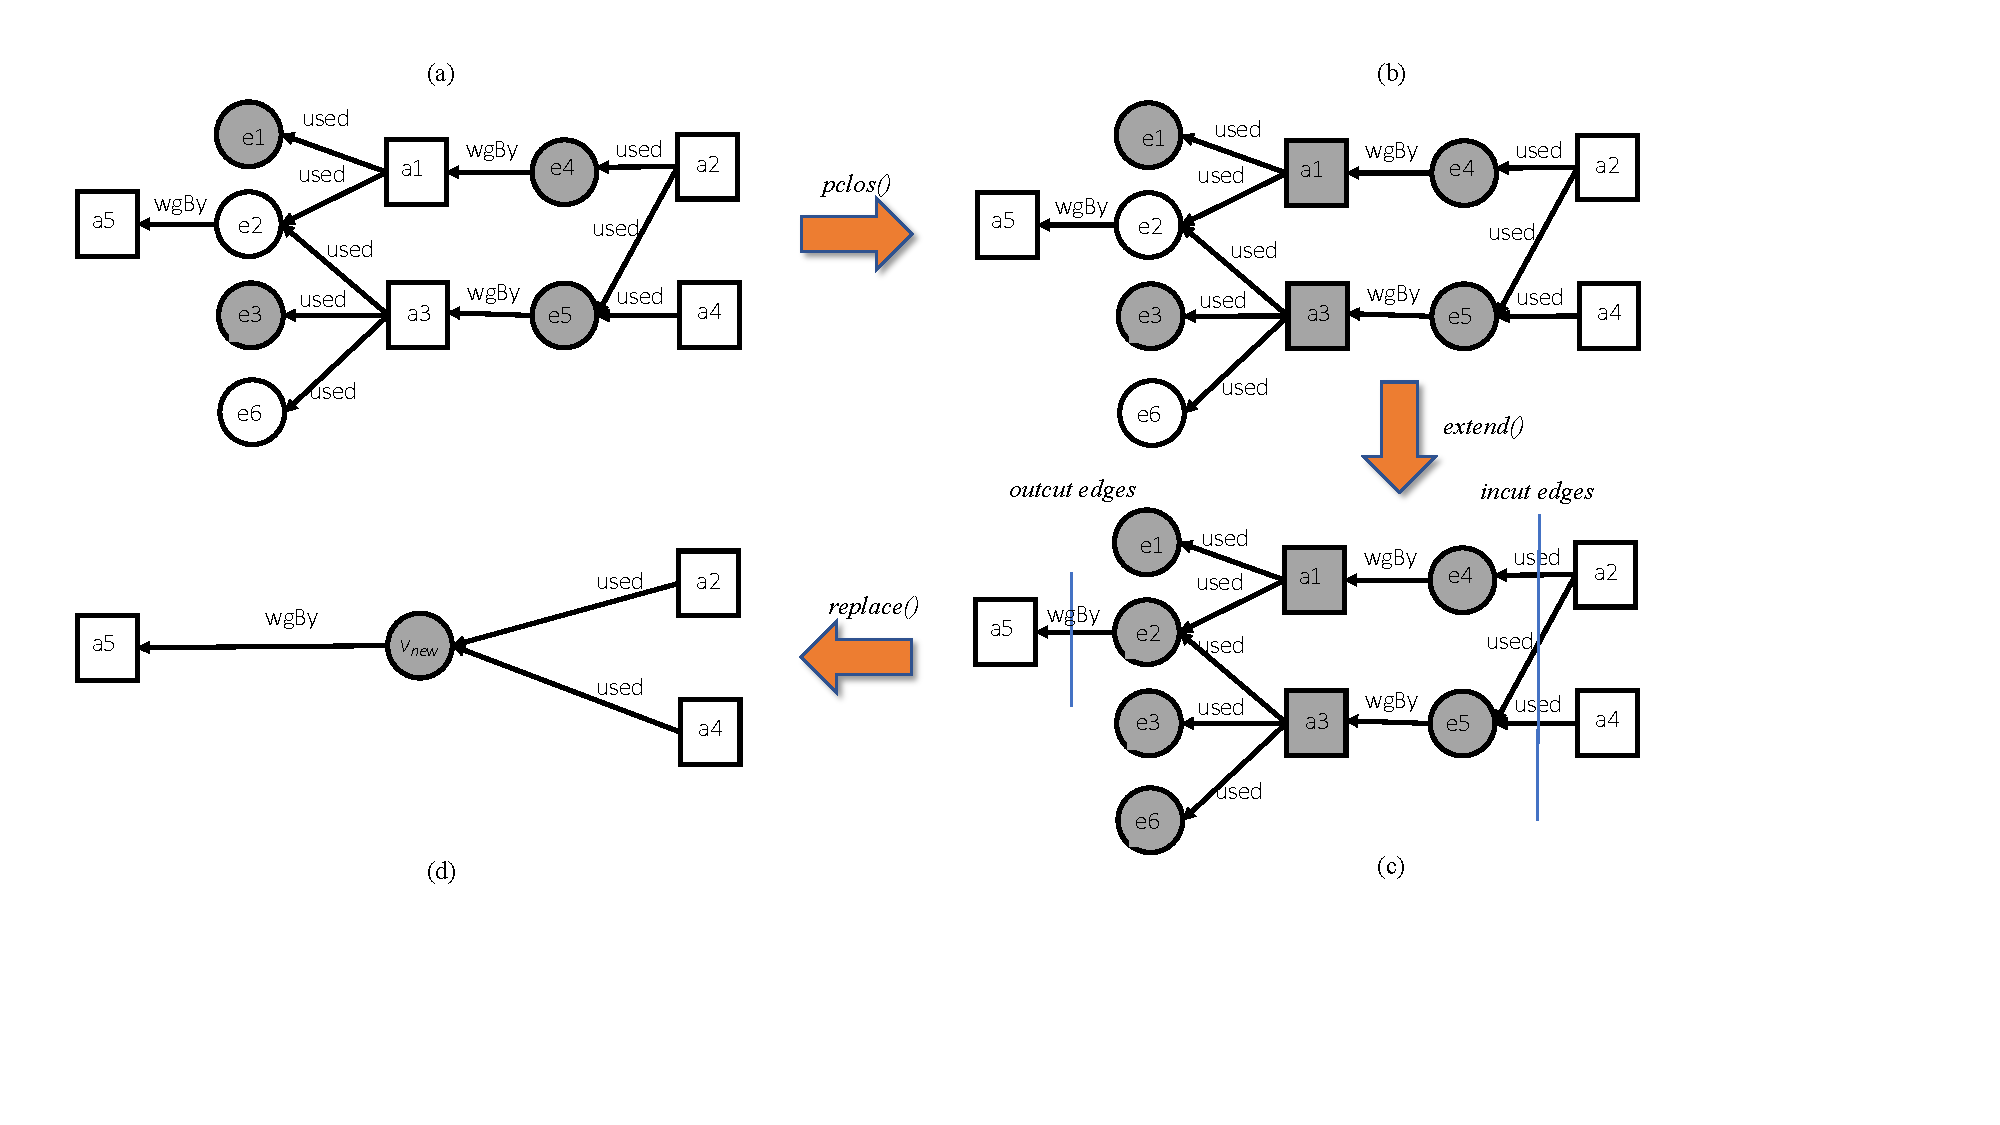
\includegraphics[scale=.5]{reworked-fig7.pdf} 
\caption{Path closure and replacement with extension on a set of entity nodes.} \label{fig:convex-ex-1}
\end{figure*}

However, \jwbtwo{ while the application of $\pclos()$ ensures that the group to be abstracted is free from cycles, simply replacing the shaded nodes in Fig.~\ref{fig:convex-ex-1}(b) with a single node $e'$ is not sufficient. This is because the resulting graph would no longer be bipartite, since the new edges $e' \rightarrow e_2$ and $e' \rightarrow e_6$ would connect nodes of the same type.}




%\jwbtwo{The purpose of the $\extend$ operator will be to ensure that 

\jwbtwo{To ensure that the eventual node replacement preserves the type-consistency of graph, we also require all the set boundary nodes (nodes in the defined set connected to nodes outside the set) to be of the same type.}
\jwbtwo{In the example in Fig.~\ref{fig:convex-ex-1} we must extend the shaded set in Fig.~\ref{fig:convex-ex-1}(b) to include e-nodes $e_2$, $e_6$, as shown in   Fig.~\ref{fig:convex-ex-1}(c). We therefore define a second operator $\extend()$ to do this.}



\jwbtwo{Formally, the application of $\extend()$ to a set $V_{gr} \subset V$ relative to type $t \in \{ \en, \act \}$ will be $V_{gr}$ augmented with all its adjacent nodes, in either direction, of type $t$.  In this way all boundary nodes of our group will have type $t$. }

%
%In this example, we can construct a new group of nodes, $\{ e', e_2, e_6\}$, on the graph that results from the first replacement, and replace it with a new node $e''$. The resulting graph \jwb{Fig.~\ref{fig:convex-ex-1}(d)} is a valid $\guEA$ graph.

%\comment{Extension}

%

%

%\comment{Following this approach, we are then free to define grouping as a composition of three functions: \textit{closure}, defined above, \textit{extension}, and \textit{replacement}, where \textit{replacement} will perform the necessary graph manipulations to provide the final abstracted graph.}

%
%\jwb{We do this because when we later replace this extended set with a single abstract node of type $t$, we want to ensure that we maintain type-correctness of the graph.}
%Formally:


%%%%
%% extension
%%%%
% \vspace*{10pt}
% \begin{definition}[$\extend$]
% Let $G = (V,E) \in \guEA$, $t \in \{ \en, \act \}$.
% \[
% \begin{array}{l}
% \extend(V_{gr}, G ,t) =  \\
% \quad V_{gr} \;\cup \\ 
% \quad    \{ v' | (v \leftarrow v') \in E \wedge v \in V_{gr} \wedge \type(v') = t \} \;\cup \\
% \quad   \{ v | (v' \leftarrow v) \in E \wedge v \in V_{gr} \wedge \jwb{\type(v) = t} \}  \\
% \end{array}
% \]
%\end{definition}
%\comment{The nodes we to which we extend must have the type $t$. It isn't possible to include a node of type other than t.}

%\comment{To make the defn below more clear, we use $v_s,v_d \nin V_{gr}$ in the definition of $extend$. This will also make this definition more compatible with the definitions of incut and outcut.}


\vspace*{10pt}
\begin{definition}[$\extend$]
  \label{def:extend}
  Let $G = (V,E) \in \guEA$, $t \in \{ \en, \act \}$. $v_s$ and $v_d$ are the source and destination nodes of a relationship.
  %\comment{we could replace $V_{gr}$ in the defn below with something that suggests $\clos$ has been applied?}
\[
\begin{array}{l}
\extend(V_{gr}, G ,t) =  \\
\quad V_{gr} \;\cup \\ 
\quad    \{ v_d | (v_d \leftarrow v_s) \in E \wedge v_s \in V_{gr} \jwb{~\wedge\ v_d \nin V_{gr}} \wedge \type(v_d) = t \} \;\cup \\
\quad   \{ v_s | (v_d \leftarrow v_s) \in E  \jwb{~\wedge\ v_s \nin V_{gr}} \wedge v_d \in V_{gr}  \wedge \jwb{\type(v_s) = t} \}  \\
\end{array}
\]


\end{definition}

%\comment{I've replaced the phrase ``sink node'' with ``boundary node'' in the following.}

%
\jwbtwo{In the example in Fig.~\ref{fig:convex-ex-1} nodes $e_2$ and $e_6$ are now included,} and 
\[
 \extend(\{e_1, e_3, e_4, e_5, a_1, a_3\}, G, \en) = \{e_1, e_3, e_4, e_5, a_1, a_3, e_2, e_6\}
\]
 as shaded in Fig.~\ref{fig:convex-ex-1}(c). 
%\jwbtwo{Note that all boundary nodes in $\extend(V_{gr}, G, t)$ are of type $t$ by construction.}
%\footnote{A boundary node is any node in the extended set with a link to a node not in the set.}

\jwbtwo{Finally, we can replace the collected nodes with a new abstract node, as shown in Fig.~\ref{fig:convex-ex-1}(d). }  \jwbtwo{The function $\repl()$ is defined to do this.}

Let $V^* \subset V$ be obtained using $\pclos()$ then $\extend()$, as outlined above, and let $v_{new}$ be a new node that does not appear in $V$.
%
Function $\repl()$ replaces $V^*$ with $v_{new}$ in $V$, and connects $v_{new}$ to the rest of the graph. 
\jwbtwo{To aid us in the definition, we begin by defining the \textit{outcut}, \textit{incut} and the \textit{internal} edges of $V^*$. The \textit{incut} and \textit{outcut} of the group of shaded nodes in Fig.~\ref{fig:convex-ex-1}(c) are marked.}




\begin{definition}
\label{def:in-out-int}
\jwbtwo{
Let $\vartheta_{out}(V^*)$ denote the \textit{outcut} of $G$ associated with $V^*$, defined as the set of arcs of $G$ pointing out of $V^*$, let $\vartheta_{in}(V^*)$ denote the \textit{incut}  of $G$ associated with $V^*$, i.e., the set of arcs of $G$ leading into $V^*$, and let $\vartheta_{int}(V^*)$ denote internal edges, that connect two nodes inside $V^*$. $\vartheta_{out}(V^*)$, $\vartheta_{in}(V^*)$ and $\vartheta_{int}(V^*)$  are given by:}

\jwbtwo{
\begin{equation*}
 \vartheta_{out}(V^*) = \{  (v_d \leftarrow v_s) |   v_s \in  V^*, v_d \in V \setminus V^*\}
\end{equation*}
\begin{equation*} 
\vartheta_{in}(V^*) = \{  (v_d\leftarrow v_s) |  v_d \in V^*, v_s \in  V \setminus V^* \}
\end{equation*} 
\begin{equation*}
\vartheta_{int}(V^*) = \{  (v_d\leftarrow v_s) | v_d, v_s \in V^*\}
\end{equation*}
}
\end{definition}

\jwb{Function $\repl()$ replaces each arc $(v_d \leftarrow v_s) \in \vartheta_{out}(V^*)$ with a new arc $(v_{d} \leftarrow v_{new})$ of the same type, and replaces each arc $(v_d \leftarrow v_s) \in \vartheta_{in}(V^*)$ with a new arc $(v_{new} \leftarrow v_{d})$ of the same type. Arcs in $\vartheta_{int}(V^*)$ simply disappear along with the nodes in $V^*$.}
%


%
\jwb{The definitions of $\vartheta_{out}'(V^*)$ and $\vartheta_{in}'(V^*)$ below define the final part of the ``rewiring'' carried out by $\repl()$. }

\begin{definition}
\label{def:var-in-out}
  Let $ty \in \{\used,  \wgby\}$. Then:
 % \begin{align*}
\begin{equation*}
\vartheta_{out}'(V^*) = \{  \jwb{(}v \xleftarrow{ty}  v_{new} \jwb{)}|  v \xleftarrow{ty} v' \in \vartheta_{out}(V^*)  
\end{equation*}
\begin{equation*}
\vartheta_{in}'(V^*) = \{  \jwb{(}v_{new} \xleftarrow{ty} v \jwb{)} | v' \xleftarrow{ty} v \in \vartheta_{in}(V^*)  
\end{equation*}
%\end{align*}
\label{def:eq:outcut}
\end{definition}

% \begin{align}
% \vartheta_{out}'(V_{gr}') = \{ & v \xleftarrow{t}  v_{new} |  v \xleftarrow{t} v' \in \vartheta_{out}(V_{gr}')  \}  \\
% \vartheta_{in}'(V_{gr}') = \{ & v_{new} \xleftarrow{t} v | v' \xleftarrow{t} v \in \vartheta_{in}(V_{gr}')  \}   \label{eq:outcut}
% \end{align}
% 

\noindent
\jwb{And the full definition of $\repl()$ is}
\vspace*{10pt}
\begin{definition}[replace]
\label{def:group-replace}

\[ \repl (V^*, v_{new}, G) = (V', E'), \mbox{ where: } \]
\begin{eqnarray*}
V' & = & V  \setminus V^*  \cup \{v_{new}\}\\
E' & = & E  \setminus (\vartheta_{out}(V^*) \cup \vartheta_{in}(V^*) \cup \vartheta_{int}(V^*))  \\
   & & \qquad \cup\  \vartheta_{out}'(V^*)  \cup \vartheta_{in}'(V^*)
\end{eqnarray*}
% \begin{align*}
% V' = V & \setminus V_{gr}  \cup \{v_{new}\}\\
% E' = E & \setminus (\vartheta_{out}(V_{gr}) \cup \vartheta_{in}(V_{gr}) \cup \vartheta_{int}(V_{gr}))  \\
%     & \cup \vartheta_{out}'(V_{gr})  \cup \vartheta_{in}'(V_{gr})
% \end{align*}
\end{definition}

It is easy to verify that the resulting graph is type-correct. All boundary nodes in \jwb{$V^*$}  are of the \jwb{same type $t \in \{En,Act\}$,} as noted above, and   $v_{new}$ \jwb{is of type $t$}  by construction.
%Thus, boundary nodes are replaced by a node $v_{new}$ of the same type.
Since the arcs have the same type as those they replace, it follows that $\repl()$ preserves type correctness.



\begin{figure*}
\centering
%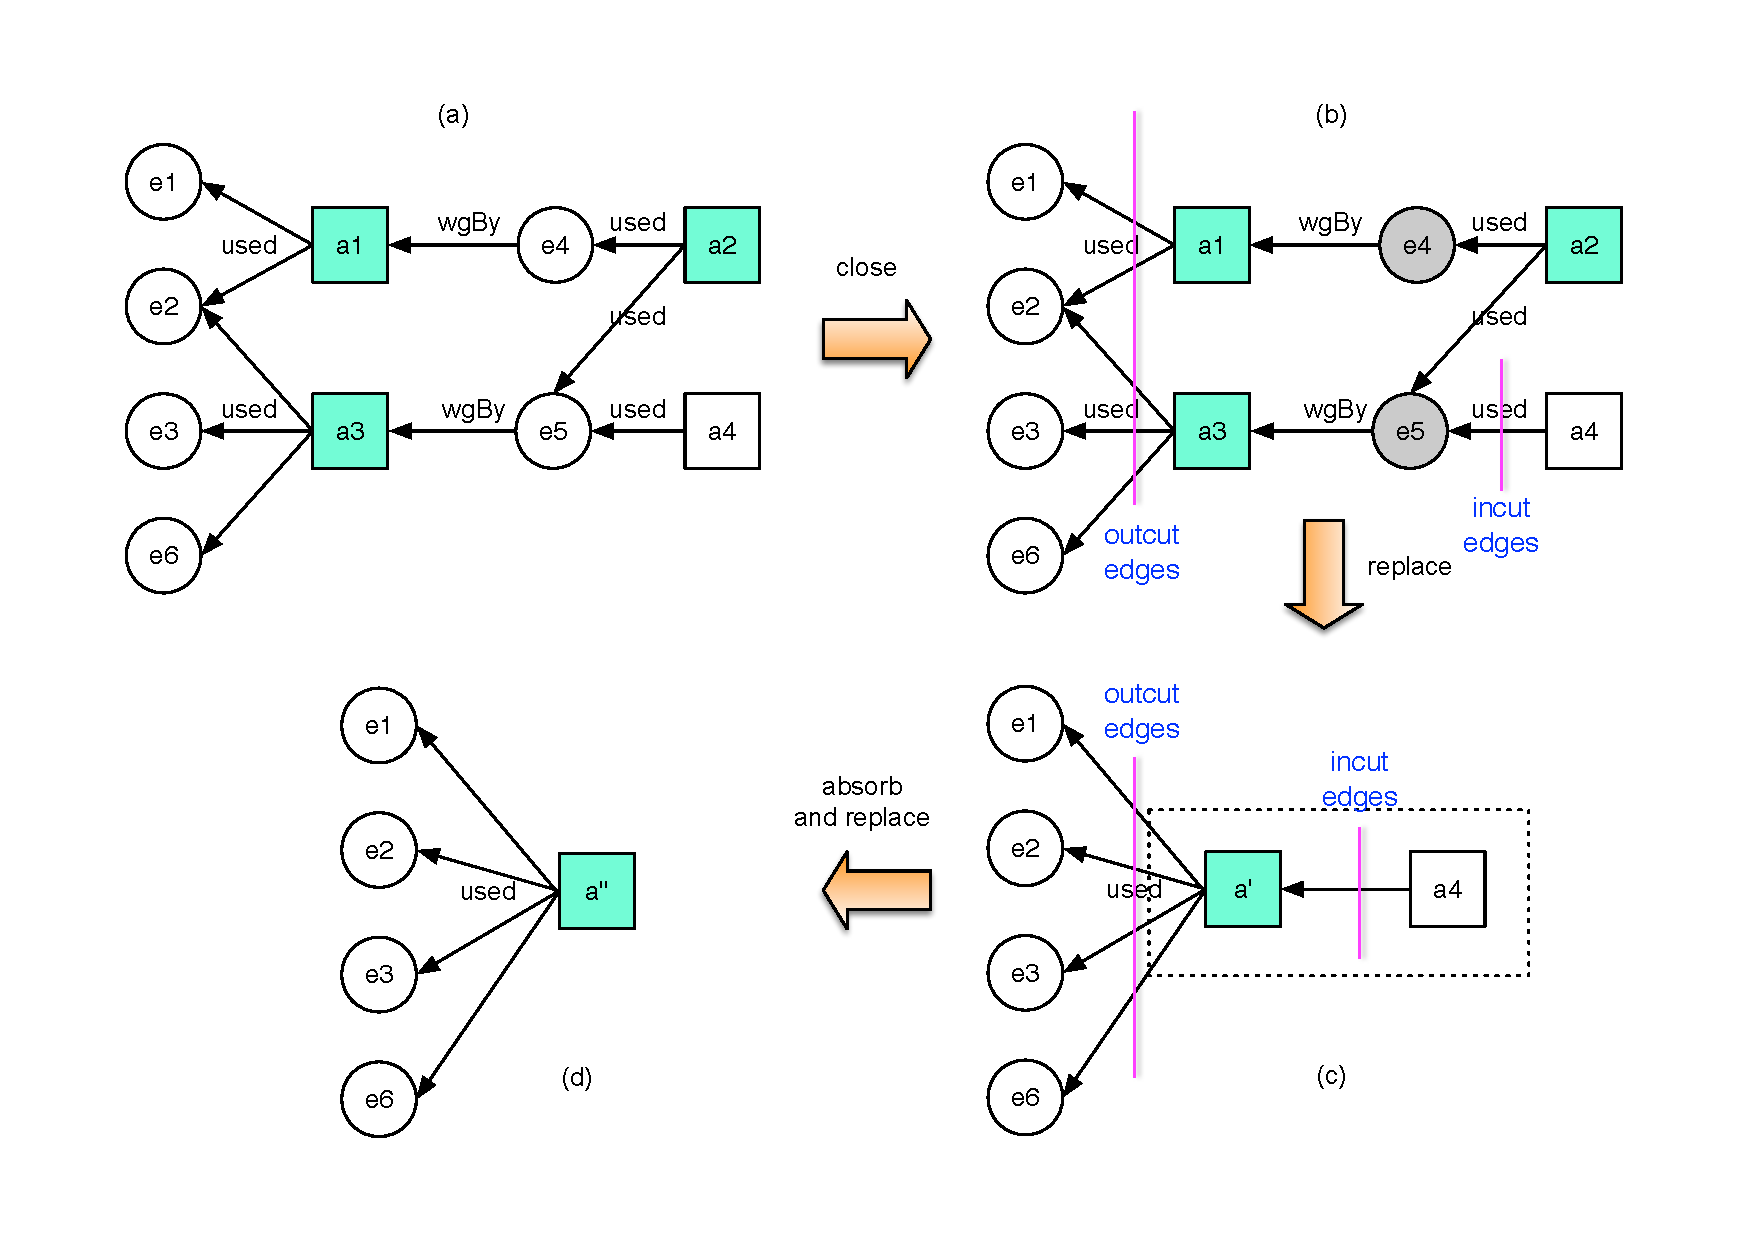
\includegraphics[scale=.5]{figures/convex-a-only-revision.pdf} 
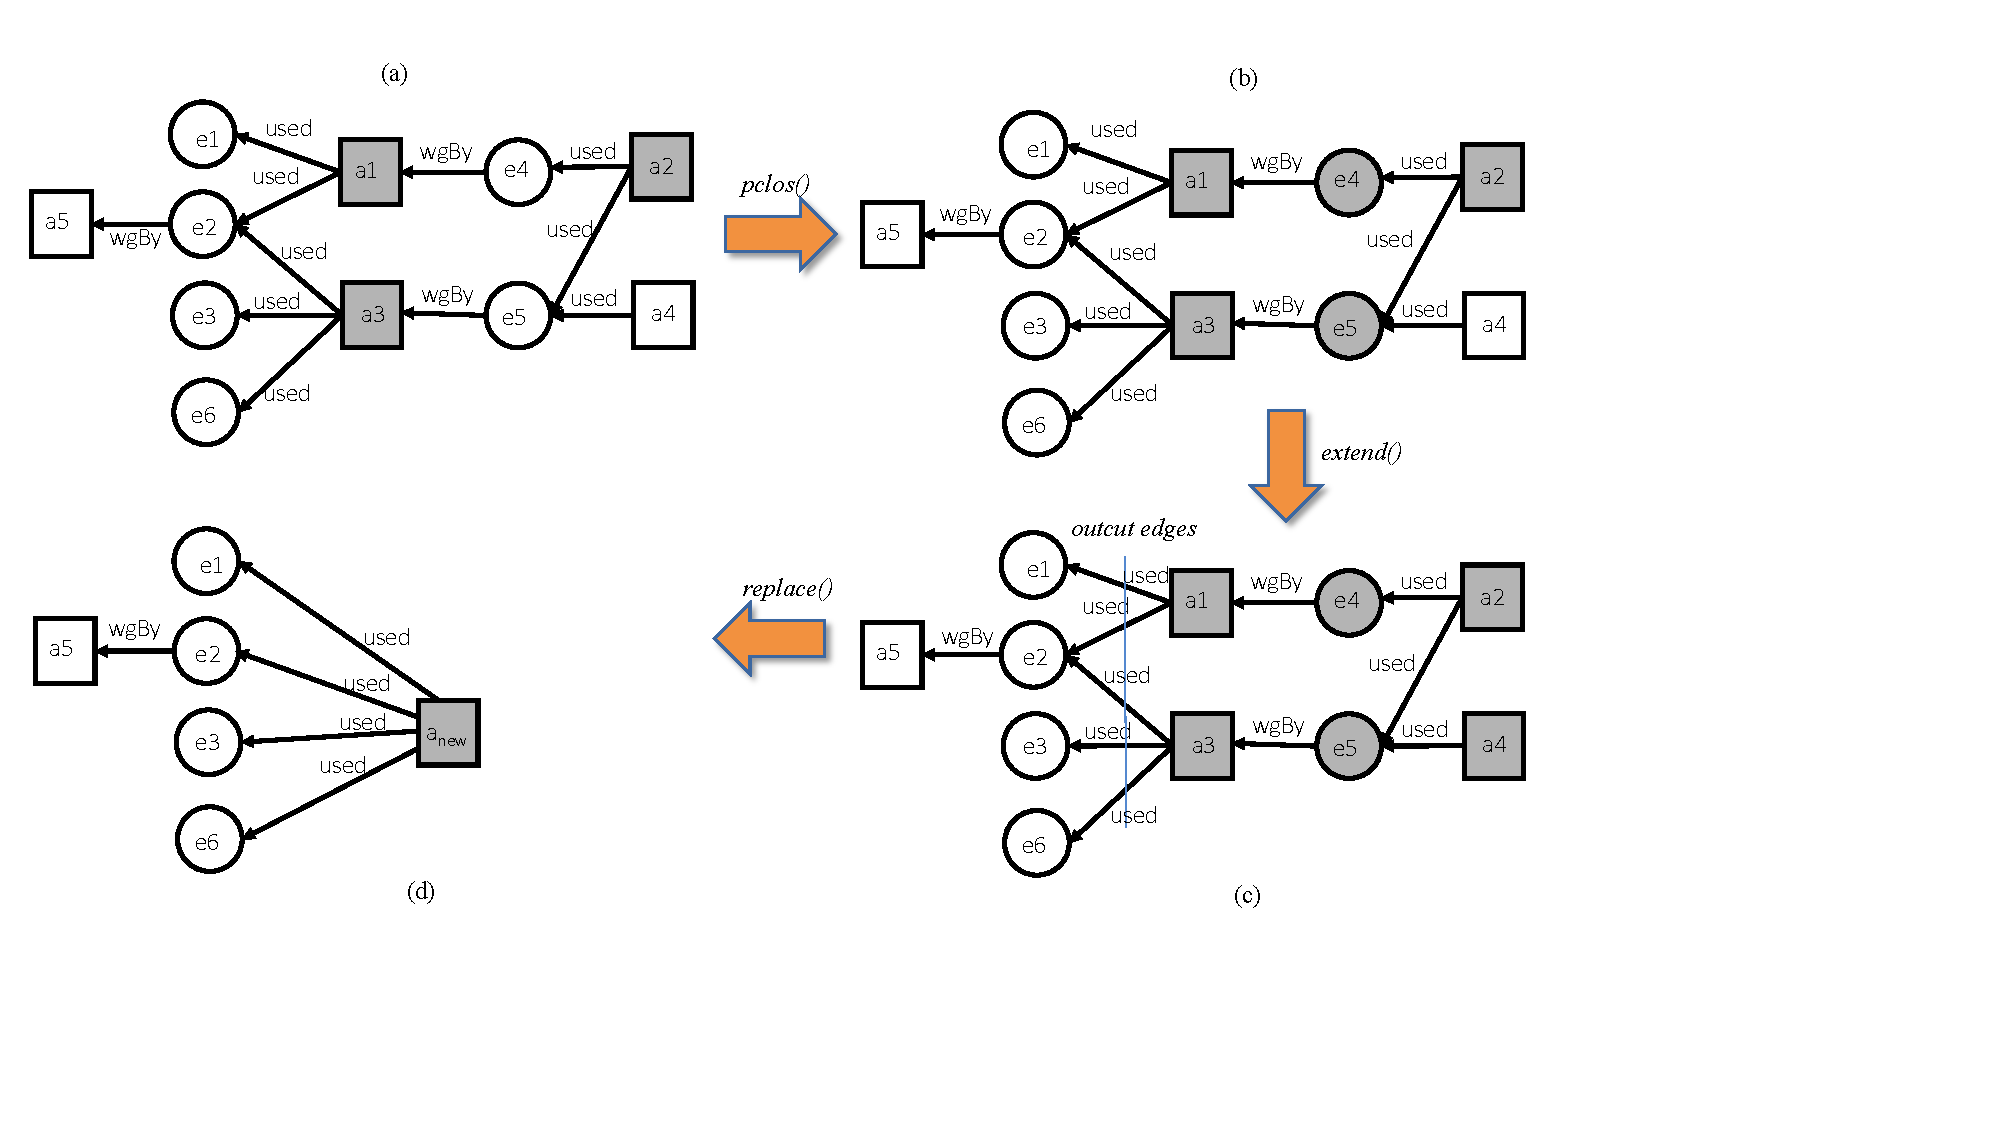
\includegraphics[scale=.5]{reworked-fig8.pdf} 
\caption{Grouping on a set of Activity nodes} \label{fig:convex-a-only}
\end{figure*}

\jwbtwo{We} now provide an initial definition of our $\group()$ operator, under the simplifying assumption that all nodes in $V_{gr}$ are of the same type \jwb{before closure.}  We denote this type by $\type(V_{gr})$ (with a slight abuse of notation), and denote the initial definition of $Group$ as $\group_{hom}$. Definitions~\ref{def:t-grouping} and~\ref{def:strict-t-grouping}  in Section~\ref{sec:generalisation} remove \jwbtwo{the assumption of type-homogeneity.}


%
Under assumption of type homogeneity, the grouping operator is a functional composition of $\clos()$, $\extend()$, and $\repl()$ functions, defined as follows.

\vspace*{10pt}
\begin{definition}[Homogeneous Grouping]
Let $G=(V,E) \in \guEA$, $V_{gr} \in V$ be a type-homogeneous set, and let $v_{new}$ be a new node with $\type(v_{new}) = \type(V_{gr})$.
\begin{align*}
\group_{hom} &  (G, V_{gr}, v_{new}) = \\
 & \repl(  \\
 & \extend( \\
 & \clos(V_{gr},\jwb{G}), V, \type(V_{gr})), v_{new},  G ) 
\end{align*}
\label{def:homo-group}
\end{definition}


Fig.~\ref{fig:convex-a-only} shows \jwbtwo{the application of $\group_{hom}$ to a set of Activity nodes. The progression is} similar to that of Fig.~\ref{fig:convex-ex-1}. This time $\type(v) = \act$ for each $v \in V_{gr} = \{a_1, a_2, a_3\}$, and $V_{gr}$ is replaced by another activity node, \jwbtwo{$a_{new}$}. 
%
\jwbtwo{The $\pclos$ operator ensures that the nodes $e_4$ and $e_5$ are included (Fig.~\ref{fig:convex-a-only}(b)), and the $\extend$ operator includes the activity node $a_4$ in Fig.~\ref{fig:convex-a-only}(c). Note that there are no incut edges: $\vartheta_{in}(V^*) = \emptyset.$  All shaded nodes are replaced with $a_{new}$ and the graph is rebuilt by the operator $\repl()$.  In the next section we remove the assumption that \jwbtwo{all the}  nodes initially selected \jwbtwo{are} of the same type.} 



%As an illustration, in the example in Figure~\ref{fig:convex-ex-1} we have: %Ive altered this example: see latex for orig.
%\begin{align*}
%V_{gr} &= \{e_1, e_3, e_4, e_5\} \\
%V_{cl} & = \clos(V_{gr},G) = \{e_1, e_3, e_4, e_5, a_1, a_3\} \\
%V^{*} & = \extend(V_{cl}, \en) = V_{cl} \cup  \{e_2, e_6 \} \\
%\group_e(G, V_{gr}, v_{new}) & = \repl(V^{*}, v_{new}, G) \\
%& = (\{a_1,a_2,a_3,e''\}, \{ (a_2, e''), (a_4, e''), (e'',a_5) \})
%\end{align*}



%\jwb{\subsubsection{Summary}}

\subsection{Generalization to \textit{e-grouping} and \textit{a-grouping}}
\label{sec:generalisation}

\jwb{So far we have described the grouping operator in terms of the component functional parts.} \jwbtwo{We} have been operating under the assumption made in Definition~\ref{def:clos}: that there is only one subgraph \jwbtwo{induced}  by  $\clos(V_{gr}, G)$.  In the case where we have two or more subgraphs,  the $\extend()$ operator and the $\repl()$ operator would iterate over the set of subgraphs produced, and be applied to each subgraph separately.


\jwbtwo{We have also been operating under the assumption of group homogeneity: that all nodes in  $V_{gr}$  are of the same type. }
Additional care must be taken if we allow $V_{gr}$ to include \jwbtwo{both node  types}.  The type of the replacement node must now be specified, as it is no longer implied from the type of the nodes in $V_{gr}$. Indeed,  the choice of the type can lead to different abstracted graphs. Thus, we will now refer to grouping as \textit{t-grouping}, where $t \in \{ \en, \act\}$, i.e., \textit{e-grouping} or \textit{a-grouping}.

\jwbtwo{Consider Fig.~\ref{fig:e2-a4}. Fig.~\ref{fig:e2-a4}(a) is a subgraph of our running  example.} 
Fig.~\ref{fig:e2-a4}(a-1, a-2) illustrates the application of the $\group_{hom}$ operator (Def.~\ref{def:homo-group}), assuming \textit{a-grouping} and $V_{gr} = \{ e_4, a_2\}$.
\jwbtwo{Although $\pclos$ has no effect, the extension incorporates activity node $a_1$ because the boundary nodes for the set to be replaced must be of type $\act$. In  Fig.~\ref{fig:e2-a4}(a-2)  $\repl$ replaces all these nodes with $a_{new}$ and edits the edges of the graph accordingly.   }


\jwb{Consider now the case of \textit{e-grouping} in Fig.~\ref{fig:e2-a4}(e-1, e-2).}  
%
\jwbtwo{Again,  $\pclos$ has no effect, but the}
   extension leads to the incorporation of $e_5$, which in turn leads to the pattern shown in Fig.~\ref{fig:e2-a4}(e-2), involving two generation events for the new entity $e_{new}$.
%\comment{do (a or e) nodes on the edge of graphs form any special cases for a- or e-grouping?  }
Although this is a valid pattern, the two generation events must be simultaneous (this is one of the temporal constraints defined in~\citep{w3c-prov-constraints}): 

%\begin{equation}
\begin{align}
ev(\wgby(e_{new}, a_1)) & \preorder ev(\wgby(e_{new}, a_3))  \quad \wedge \\
ev(\wgby(e_{new}, a_3)) & \preorder ev(\wgby(e_{new}, a_1))
\end{align}
%\end{equation}
The intuitive interpretation for this pattern is that each of the two activities generated one entity in the group represented by $e_{new}$, and that the abstraction makes these two events indistinguishable.  Formally, nothing further needs to be done to the graph. \jwb{We will explore the implications of the event ordering rules further in Section~\ref{sec:event}.  }  However note that one can restore, if desired, the more natural pattern whereby one single generation event is recorded for $e_{new}$. This is achieved simply by \jwbtwo{extending} the grouping to the set of generating activities.
In the example, this leads to the graph in Fig.~\ref{fig:e2-a4}(e-3).  

\begin{figure*}
\centering
%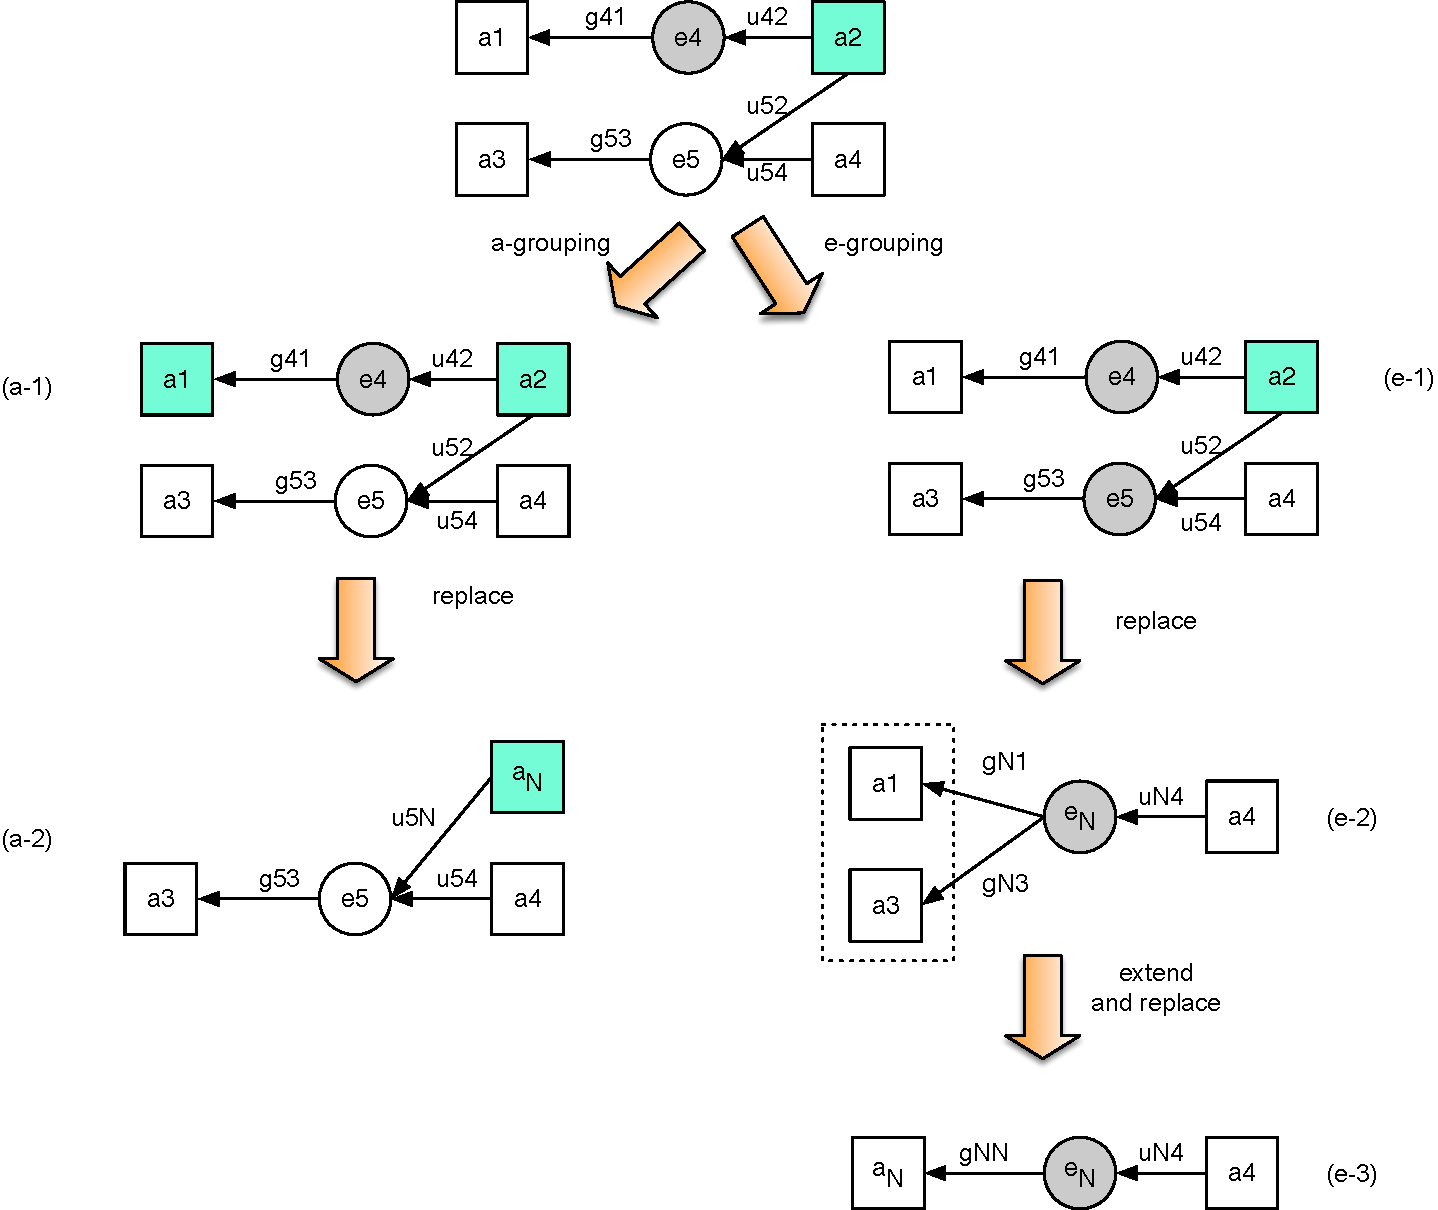
\includegraphics[scale=.25]{figures/e2-a4.pdf} 
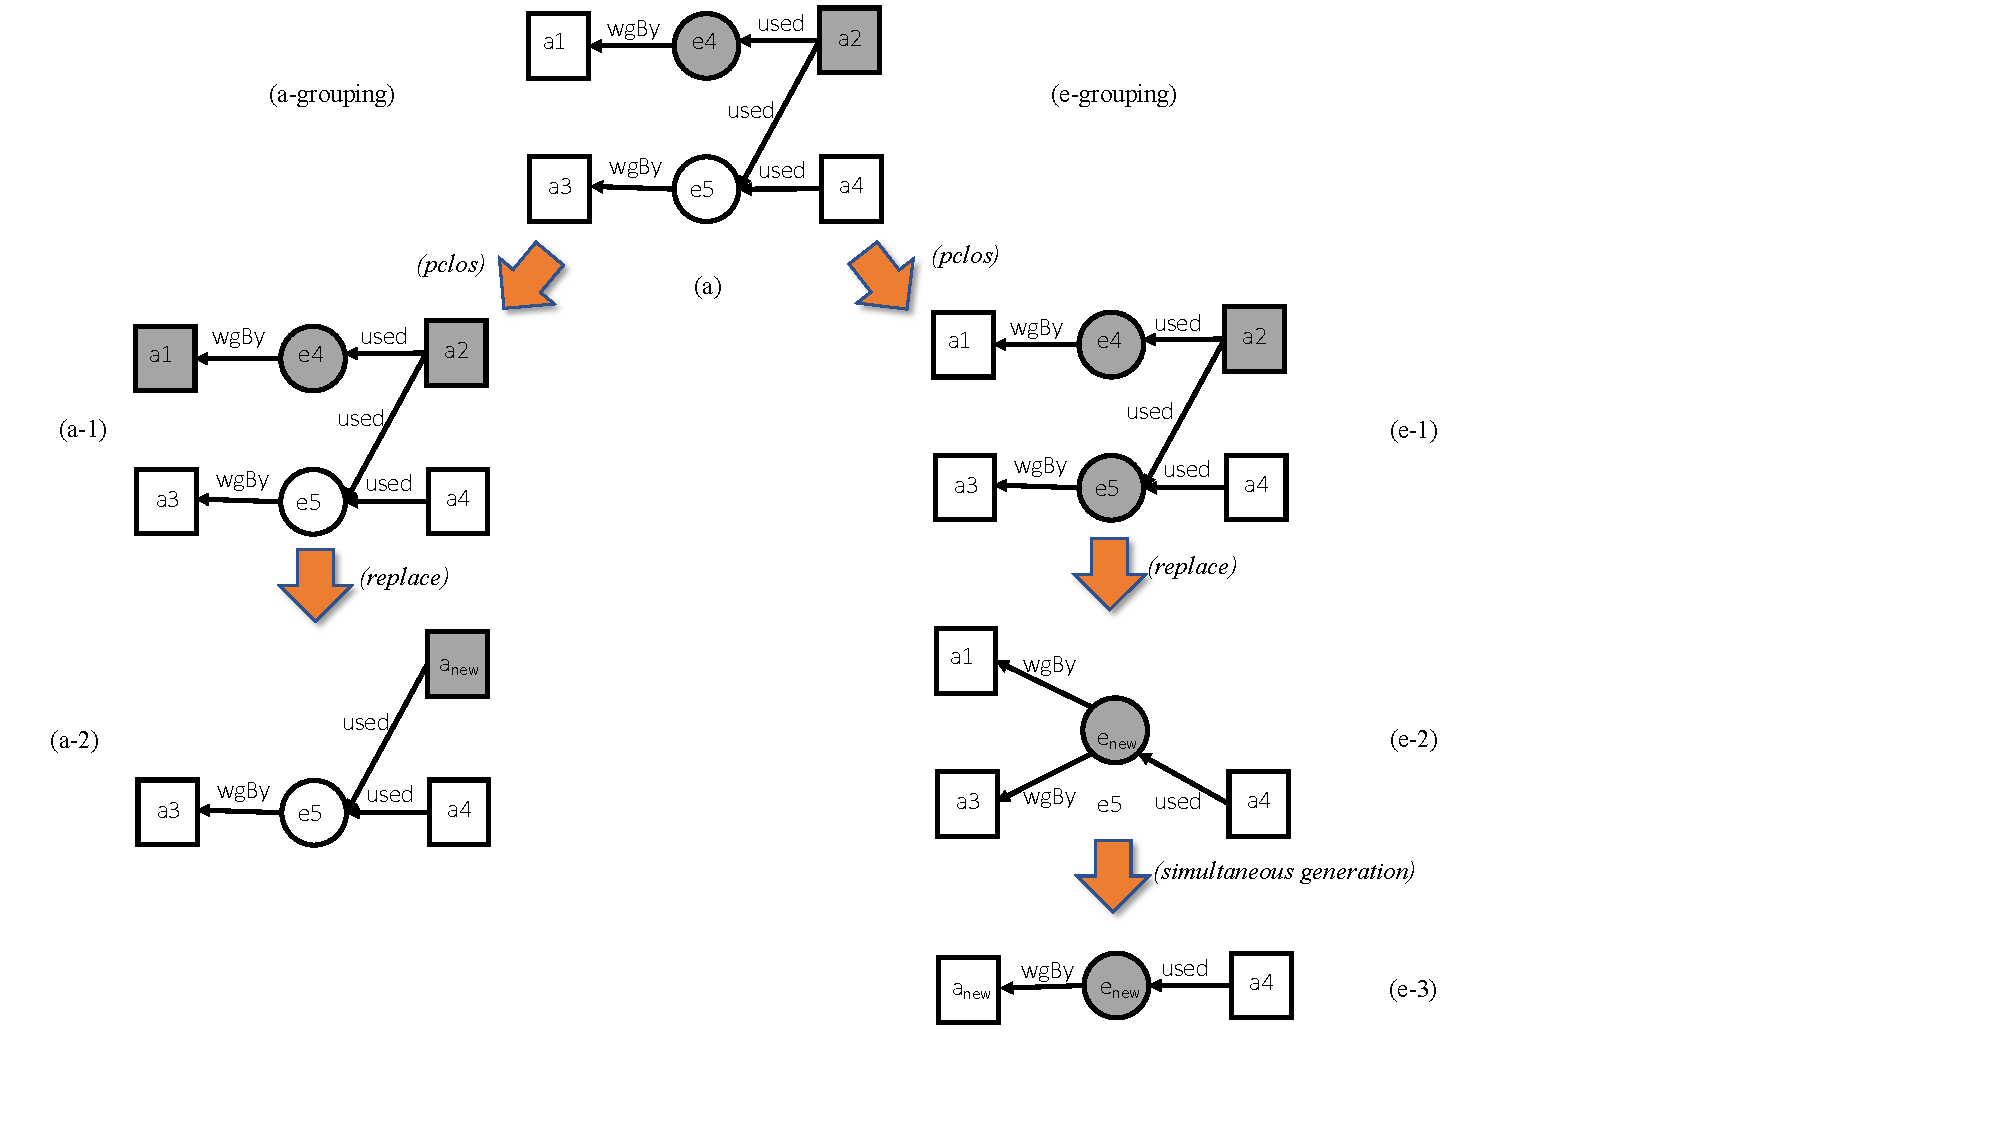
\includegraphics[scale=.5]{reworked-fig9.pdf} 
\caption{e-grouping and a-grouping on mixed type nodes} \label{fig:e2-a4}
\end{figure*}

We now formalize these considerations by introducing two definitions for $\group$. The first, which we call \textit{t-grouping} \jwbtwo{where $t \in \{\en,\act\}$}, is agnostic of multiple generation patterns, while the second (\textit{strict e-grouping}) applies \jwbtwo{a further step to e-grouping} to ensure that the \jwbtwo{new} graph is free from multiple generation patterns. \jwbtwo{Note that a-grouping does not need a similar strict version, since the new node, an activity, does not have the possibility of multiple generation. }

\vspace{10pt}
\begin{definition}[t-Grouping]
\label{def:t-grouping}
Let $G=(V,E) \in \guEA$, $V_{gr} \in V$, $t \in \{\en, \act\}$, and let  $v_{new}$ be a new node with $\type(v_{new}) = t$.
%
Then:
\begin{align*} 
\group & (G, V_{gr}, v_{new}, t) = \\
& \repl( \extend(\clos(V_{gr},\jwb{G}), V, t), v_{new},  G )
\end{align*}
\label{eq:t-grouping}
\end{definition}

Note that the assumption that \jwb{boundary} nodes in the closure are homogeneous still holds in this case. 

\jwbtwo{Strict e-grouping} performs the further step illustrated in the transition from Fig.~\ref{fig:e2-a4}(e-2) to Fig.~\ref{fig:e2-a4}(e-3). \jwbtwo{Note that that the $Group$ operator can only produce a multiple generation pattern if $type(v_{new})=En$.}


%\comment{need to remove any  genBy}


\begin{definition}[Strict e-Grouping]
Given 
$G=(V,E) \in \guEA$, $V_{gr} \in V$, $t \in \{\en, \act\}$, and a new node $v_{new}$ with $\type(v_{new}) = \en$, let
\[ G' = (V',E') = \group(G, V_{gr}, v_{new}, \en). \]
Let 
$V_{gen} = \{ a \in V' |  a \xleftarrow{\wgby} v_{new} \in E' \}$ be the set of activity nodes that generate $v_{new}$ according to $G'$, and let $a_{new}$ be a new activity node. Then:
\begin{equation*}
%\footnotesize
\sgroup(G, V_{gr},v_{new}, t)=
\begin{cases}
G' & \!\text{if}~~ |\!\!V_{gen}\!| ~~\leq 1  \\
\repl(V_{gen}, a_{new}, G') & \!\text{otherwise } 
\end{cases}
%\normalsize
\end{equation*}
\label{def:strict-t-grouping}
\end{definition}
%
%It is straightforward to show that strict t-grouping reduces to normal grouping if the grouping is a homogeneous a-grouping:
%\begin{align*}
%&\text{if } \type(t) =  \act \\
% &\qquad\text{then } \sgroup(G, V_{gr},t) = \group(G, V_{gr},t). 
%\end{align*}


%
%
%In addition, however, they are also subject to ordering constraints relative to events associated to elements in in $V_{cl}$ (the set of nodes to be grouped, resulting from Path Closure on source graph $G'$), which have now been replaced by the grouping nodes. To illustrate this reasoning, consider for instance the simple graph in Fig.~\ref{fig:simple-prototype-pattern-events}(a), and let $V_{gr}= \{ e_1, e_2\}$. The ordering constraints on $G$ are as follows:
%
%
%\begin{figure}
%\centering
%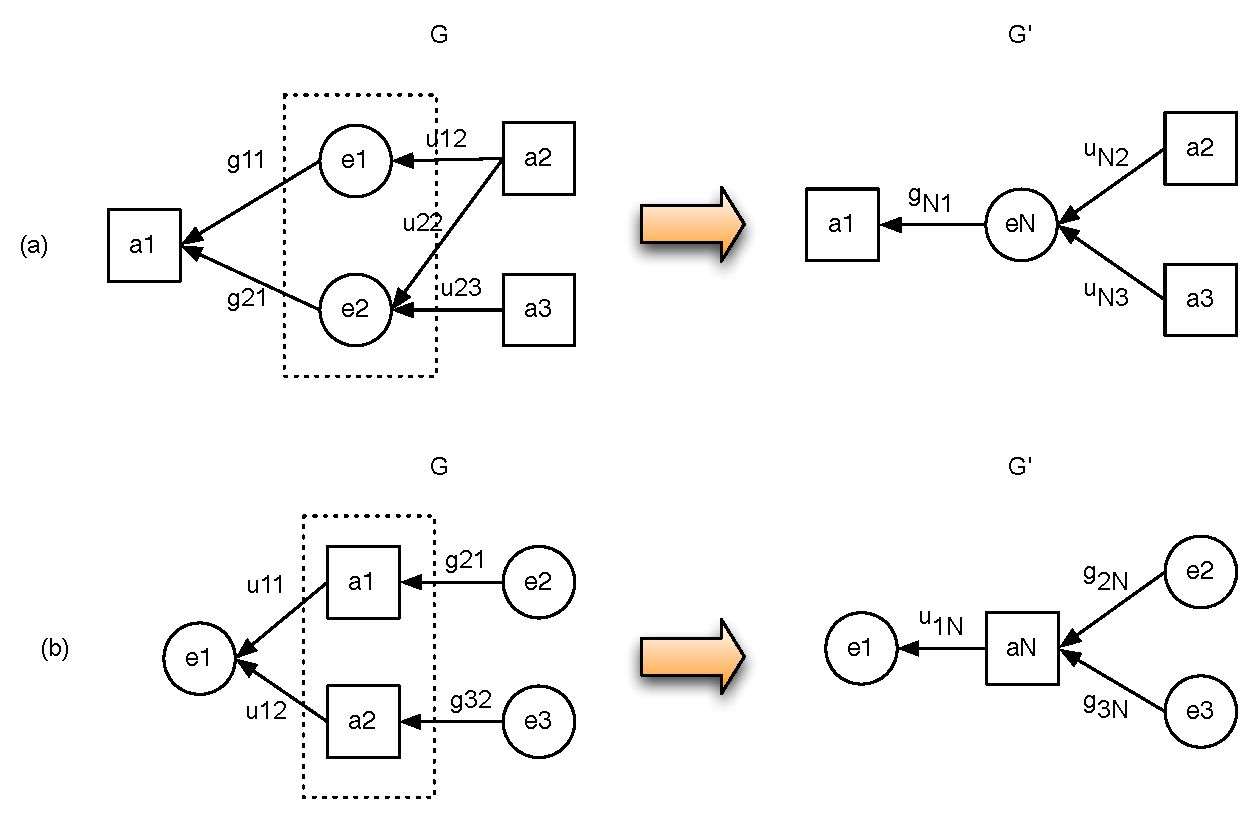
\includegraphics[scale=.5]{figures/simple-prototype-pattern-events} 
%\caption{Simple graph patterns to illustrate ordering constraints on events after grouping} \label{fig:simple-prototype-pattern-events}
%\end{figure}
%
%
%\begin{align*}
%start_{ev}(a_1) \preorder gen_{ev}(\wgby(e_i, a_1)) \preorder end_{ev}(a_1)   \text{ for } i=1, i=2\\
%start_{ev}(a_2) \preorder usage_{ev}(\used(a_2,e_1)) \preorder end_{ev}(a_2) \\
%start_{ev}(a_j) \preorder usage_{ev}(\used(a_j,e_2)) \preorder end_{ev}(a_j) \text{ for } j=2, j=3 \\
%gen_{ev}(\wgby(e_2, a_1))  \preorder usage_{ev}(\used(a_j,e_2))  \text{ for } j=1, j=2 \\
%gen_{ev}(\wgby(e_1, a_1))  \preorder usage_{ev}(\used(a_2,e_1)) \\
%\end{align*}
%%
%The corresponding ordering constraints on $G'$ are as follows.
%%
%\begin{align}
%start_{ev}(a_1) \preorder gen_{ev}(\wgby(e_N, a_1)) \preorder end_{ev}(a_1)  \label{eq:constraints-example-1}  \\
%start_{ev}(a_2) \preorder usage_{ev}(\used(a_2, e_N)) \preorder end_{ev}(a_2) \\
%start_{ev}(a_3) \preorder usage_{ev}(\used(a_3, e_N)) \preorder end_{ev}(a_3) \\
%gen_{ev}(\wgby(e_N, a_1))  \preorder usage_{ev}(\used(a_2,e_N)) \\
%gen_{ev}(\wgby(e_N, a_1))  \preorder usage_{ev}(\used(a_3,e_N)) \label{eq:constraints-example-n} 
%\end{align}
%
%The following additional ordering constraints further characterize events in $G'$ in terms of events in $G$. It is easy to see that such constraints are sufficient conditions for the constraints \ref{eq:constraints-example-1}-\ref{eq:constraints-example-n} above to hold.
%\begin{align*}
%usage_{ev}(\used(a_2,e_1)) \preorder usage_{ev}(\used(a_2,e_N))  \\
%usage_{ev}(\used(a_2,e_2)) \preorder usage_{ev}(\used(a_2,e_N)) \\
%usage_{ev}(\used(a_3,e_3)) \preorder usage_{ev}(\used(a_3,e_N)) \\
%gen_{ev}(\wgby(e_N, a_1)) \preorder gen_{ev}(\wgby(e_1, a_1)) \\
%gen_{ev}(\wgby(e_N, a_1)) \preorder gen_{ev}(\wgby(e_2, a_1)) )
%\end{align*}
%
%A similar reasoning applies to the case of a-grouping, illustrated in Fig.~\ref{fig:simple-prototype-pattern-events}(b), where the following definitions are consistent with the temporal orderings:
%\begin{align*}
%usage_{ev}(\used(a_1,e_1)) \preorder usage_{ev}(\used(a_N,e_1))  \\
%usage_{ev}(\used(a_2,e_1) ) \preorder usage_{ev}(\used(a_N,e_1))  \\
%gen_{ev}(\wgby(e_2, a_N))  \preorder  gen_{ev}(\wgby(e_2, a_1)) \\
%gen_{ev}(\wgby(e_3, a_N))  \preorder gen_{ev}(\wgby(e_3, a_2)) \\
%start_{ev}(a_N) \preorder start_{ev}(a_1) \\
%start_{ev}(a_N) \preorder  start_{ev}(a_2) ) \\
%end_{ev}(a_1) \preorder end_{ev}(a_N)  \\
%end_{ev}(a_2) ) \preorder end_{ev}(a_N)  
%\end{align*}
%
%Following this reasoning, we define the following additional ordering constraints amongst events in $G'$ and $G$ events.

%\begin{figure}
%\centering
%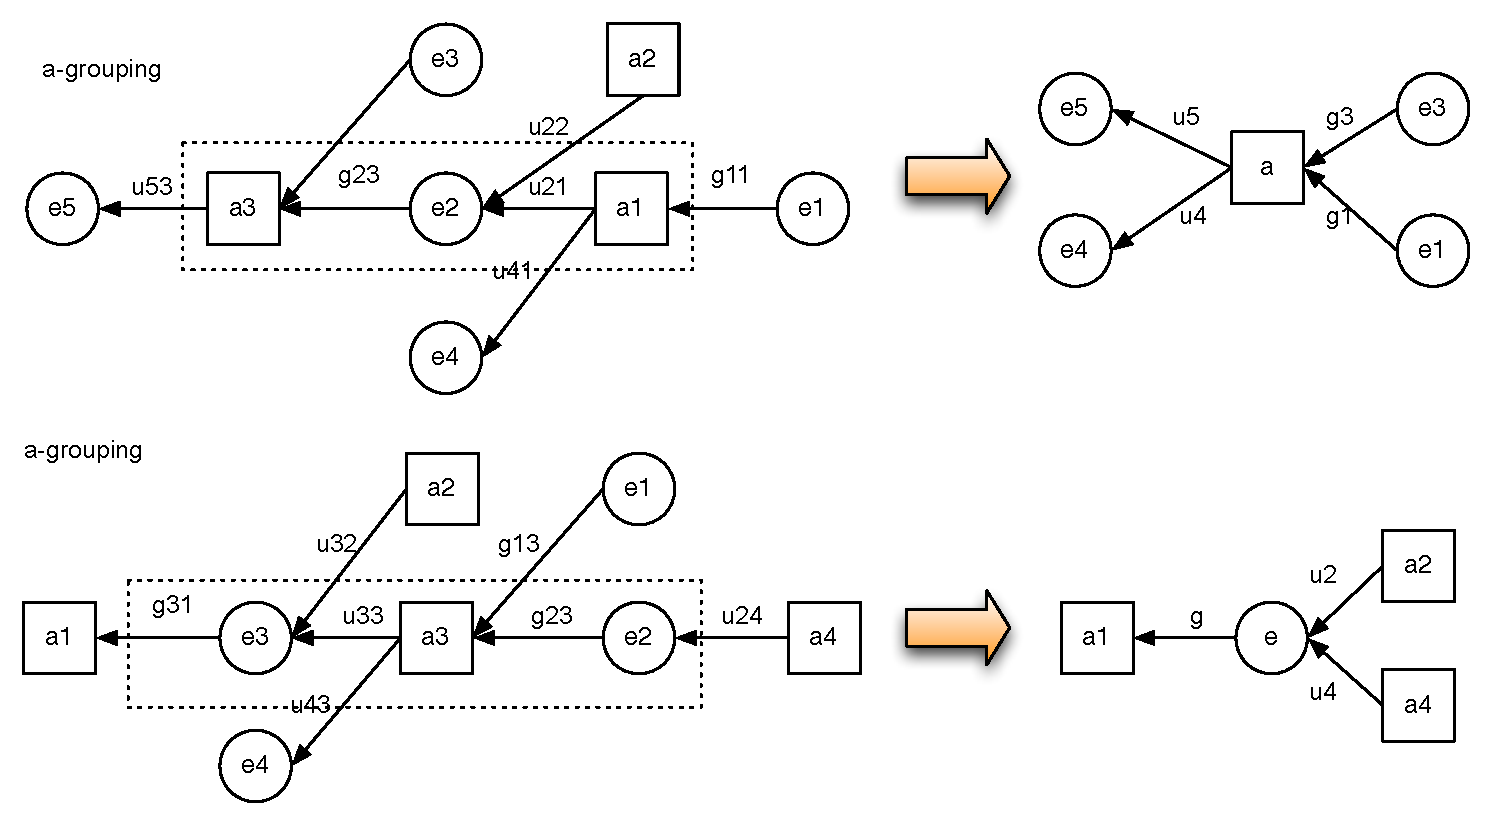
\includegraphics[scale=.5]{figures/a-grouping-pattern-proofs} 
%\caption{$\guEA$ graph patterns for e- and a-grouping} \label{fig:a-grouping-pattern-proofs}
%\end{figure}

% \jwb{
% \subsection{Multiple Applications of Group}
% \label{sec:allowing}
% }
% 
% \comment{replace iterates over all subgroups. this bit not needed. }
% \comment{the most general case produces two or more disjoint subgraphs (where disconnect means there is no path from any node in one to any node in the other  }
% 
% \jwb{In this section we relax the assumption made after Definition~\ref{def:clos}, that the subgraph identified by  $\pclos(V_{gr},G)$ is connected.}
% %
% \jwb{If, instead,  two separate subgraphs are identified within $\pclos(V_{gr},G)$, there are two possibilities. Either following the application of $\extend$ (which extends the set of nodes encompassed) the two subgraphs remain separate, in which case they should be treated as two graphs, or following the applications of $\extend$ the two subgraphs overlap. }
% %
%   \jwb{In this case, we must show that the order in which the $\repl$ functions are carried out is unimportant.}
%   %
%   \jwb{Note that, because it was only at the point of using $\extend$ that the graphs overlapped, we only need to consider the order of application of the two $\repl$ functions.}
% 
% \begin{theorem}\label{thm:multiple}
% \jwb{Let $V_1 \inter V_2 \neq \emptyset$. It is the case that
%    \[
%   \repl(V_1,v_n,\repl(V_2,v_m,G)) =   \repl(V_2,v_m,\repl(V_1,v_n,G))
%   \]}
% \noindent
% \end{theorem}
% \jwb{Proof:~\ref{app:multiple}.}
%


\subsection{Justifying relations}
\label{sec:justifying}

\jwbtwo{In this section, we clarify what it means to say that relations in the abstract graph are justified, and show that the relations produced by the $\group$ operator (more properly, the family of $\group$ operators) are justified.} 



\begin{definition}
\label{def:justify}
\jwbtwo{
A abstract node is justified by the concrete graph if (i) it appears unchanged in the concrete graph, or (ii) it is a new node representing a set of concrete nodes, and one of the concrete nodes has the same type as the abstract node.
%
An abstract relation between two nodes is justified if (i) the nodes are justified (in the sense above) and (ii) the type of the abstract relation is unchanged. 
%
An abstract graph is justified if the nodes and relations in it are justified. }
\end{definition}



 
\jwbtwo{To see that the $\group$ operator produces justified abstract graphs, consider two graphs: a concrete one, $C$, represented by the graph $G_C = (V_C,E_C)$, and an abstract one $A$, represented by the graph $G_A = (V_A,E_A)$.
If $(v^A_d \xleftarrow{t} v^A_s)$ is a relation in $E_A$ of type $t$,  we need to show that there is a justifying relation $(v^C_{d'} \xleftarrow{t'} v^C_{s'})$ in $E_C$. Observe too that the $\group$ operator removes some nodes from $G_C$ but produces only one new node $v_{new}$ in $G_A$, so there are three cases to consider. Either (i) the relation is unchanged, so 
$v^A_d = v^C_{d'}, t=t'$ and $v^A_s = v^C_{s'}$;
(ii) one of the source or the destination node is a new (and therefore abstract) node which the $Group$ operator has inserted as a replacement for a set of nodes, and the other node is unchanged.
In all cases the type of the relation must be unchanged, so $t=t'$. }



\jwbtwo{To see that relations are justified in this sense, consider how the nodes  $v^A_d$ and $v^A_s$  in $(v^A_d \xleftarrow{t} v^A_s)$  were identified.
%
% Inspection of Definition~\ref{def:group-replace} shows three possibilities: (i) $v^A_s$ is $v_{new}$, and $v^A_d$ is unchanged (ie $v^A_d = v^C_d$), (ii)  $v^A_d$ is $v_{new}$, and $v^A_s$ is unchanged (ie $v^A_s = v^C_s$), or (iii) both $v^A_s$ and $v^A_d$ are unchanged from the concrete graph, so $v^A_s = v^C_s$ and $v^A_d = v^C_d$.
}

\jwbtwo{
Considering case (i) first, we need to show that the type of the relation remains unchanged during the abstraction operation. But since $v^A_s$ and $v^A_d$ have not changed from the concrete graph, we know that $v^C_s, v^C_d \in V \setminus V^*$. }
\jwbtwo{
From this, and observation of Definition~\ref{def:in-out-int},  it follows that none of 
$\vartheta_{out}(V^*)$,
$\vartheta_{in}(V^*)$, and $\vartheta_{int}(V^*)$   apply  and so, by Definition~\ref{def:group-replace}, neither $v^A_s$ or $v^A_d$ is removed from $V_C$ in the transformation by $\group$ to $V_A$. Thus the relationship is maintained in $E_A$, and the type of the relation in $E_A$ does not change,  $t=t'$.
}

\jwbtwo{
Consider next case (ii), in which  $v^A_d$ is the new node $v_{new}$ and $v^A_s$ is unchanged. In this case, to justify the new relation, we need to show that there is a relation $(v^C_{d'} \xleftarrow{t'} v^C_{s'})$  in $E$, and that the operation of $\group$ produces the relation $(v_{new} \xleftarrow{t} v^A_{s})$ in $E_A$, where $V^A_s = V^C_{s'}$ and $t=t'$. 
%
We see this by considering the definition of $\vartheta_{in}(V^*)$ in Definition~\ref{def:in-out-int}. The source of the relation is unchanged, since $v_s \in V\setminus V^*$, so it is not in the set $V^*$ that has been chosen to be abstracted. 
The type of $v_{new}$ is given by the type of the boundary nodes in $V^*$, and
the replacement relation is given by the definition of $\vartheta'_{in}(V^*)$ in Definition~\ref{def:var-in-out}, from which we see that the source and type of the relation are unchanged in $E_A$.
}

\jwbtwo{
Case (iii) is exactly similar, except that $v^A_s$ is the new node $v_{new}$ and $v^A_d$ is unchanged, and follows from inspection of $\vartheta_{out}(V^*)$ and $\vartheta'_{out}(V^*)$. 
} 

\jwbtwo{To see that this reasoning applies across all group operators ($group_{hom}$, t-grouping, e-grouping and strict e-grouping), observe that the definitions called upon in the reasoning above are the definitions of $\vartheta_{in},  \vartheta_{out}, \vartheta_{int}, \vartheta'_{in}$, and $\vartheta'_{out}$ in  Definitions~\ref{def:in-out-int} and ~\ref{def:var-in-out}, and the definition of $\repl$ in Definition~\ref{def:group-replace}, and that these do not change across any of the grouping operators. 
}

%\comment{boundary nodes}



\subsection{Complexity of grouping operators}  \label{sec:complexity}

\paolo{
The grouping operator ensures that the validity of a PROV graph is preserved, that is, the abstracted graph that results from a valid PROV graph does not violate PROV constraints.
Such a guarantee, however, comes at a cost which is defined by the complexity of the $\pclos()$ and $\extend()$ operators.
Here we analyse their worst-case complexity, and then argue that much better performance is expected in practical cases.
}
\paolo{
Firstly, observe that the closure operator can be reduced to a special case of the node reachability problem for acyclic digraphs.
Specifically, given two nodes $v_1, v_2 \in V_{gr}$ such that $v_1$ is reachable from $v_2$, we need to collect all nodes along \textit{all} paths that connect $v_1$ to $v_2$.
This can be accomplished by enumerating all nodes $x$ that are reachable from each $v \in V_{gr}$ while keeping track of the corresponding paths. Whenever $ x \in V_{gr}$, we collect all nodes along the recorded path from $v$ to $x$.
}

\paolo{
It is easy to see that the worst-case scenario occurs when the nodes in $V_{gr}$ are located at the two ends of the graph, i.e., they are either source or sink nodes.
In such case, the reachability algorithm needs to visit \textit{all} nodes $V$ and \textit{all} edges $E$ in the graph, and it must additionally keep track of all edges it traverses.
}

\paolo{
Using a simple BFS approach,  we can solve the reachability problem in $O(\mid V\mid + |E|)$ steps, which in the worst-case is $O(|V|^2)$, with $O(\mid E\mid)$ space complexity for recording all edges. 
Note that the many algorithms that exist to address the problem aim to strike a balance between the cost of pre-processing the graph in order to efficiently answer multiple reachability queries, and the complexity of each individual query.
In our case, however, we can dispense with pre-processing as we expect the closure over $V_{gr}$ to be computed only once.\footnote{Note however that, when consecutive abstraction rounds are envisioned, i.e., abstraction over abstracted graphs, pre-processing may be appropriate, but that needs to be balanced against the cost of updating the data structures after each abstraction round.}
}

\paolo{
An experimental evaluation of the actual cost of computing closures in practice is beyond the scope of this paper, which is focused on the theoretical underpinnnings of the abstraction operations.
However, two factors suggest that the practical complexity will be considerably less than the worst-case.
Firstly, we can stop the graph traversal as soon as we have visited all $V_{gr}$ nodes. Unless one of those is a sink node, this results in pruning part of the graph. 
Note also that in this case the abstraction will consist of one single abstract node that represents the entire graph, because the closure will include all nodes, which is unlikely to be a desired outcome.
And secondly, in a \jwbtwo{$\guEA$} graph not all edges are allowed, in fact \jwbtwo{$\guEA$ graphs are} bipartite with respect \jwbtwo{to} the nodes types (entities and activities). Furthermore, there is at most one generating activity per entity. These factors greatly reduce the expected number of edges to much less than the theoretical \jwbtwo{maximum} $|V|^2$.
}

\paolo{
Regarding the $\extend()$ operator, note that this requires all nodes in $\pclos(V_{gr}, G)$ to be visited in order to check their type and possibly extend the closure to their immediate successors. 
This is a linear problem in the worst case, namely when the closure contains all nodes in the graph (in practice, we expect the closure to be much smalller than the graph).
%}
}

\subsection{An alternative ``lossy'' approach to abstraction}  \label{sec:influence}

\paolotwo{
Our entire approach is based on the premise that we aim to preserve the original $\used$ and $\wgby$ relationships, possibly at the expense of incorporating additional nodes into the abstraction, i.e., by means of the $\extend()$ operator.
For completeness, we mention here one alternative approach involving PROV's influence relationship: \textit{An influence relation between two objects $o_2$ and $o_1$ is a generic dependency of $o_2$ on $o_1$ that signifies some form of influence of $o_1$ on $o_2$}\footnote{https://www.w3.org/TR/prov-dm/\#term-influence}.
}

\paolotwo{Our entire approach is based on the premise that we aim to preserve the original $\used$ and $\wgby$ relationships, possibly at the expense of incorporating additional nodes into the abstraction, i.e., by means of the $\extend()$ operator.
For completeness, we mention here one alternative approach involving PROV's influence relationship: \textit{An influence relation between two objects $o_2$ and $o_1$ is a generic dependency of $o_2$ on $o_1$ that signifies some form of influence of $o_1$ on $o_2$}\footnote{https://www.w3.org/TR/prov-dm/\#term-influence}.}

\paolotwo{The generic nature of the influence relationship, denoted $\influence$, is captured formally in the PROV-CONSTRAINTS document~\citep{w3c-prov-constraints}, specifically Inference 15\footnote{https://www.w3.org/TR/2013/REC-prov-constraints-20130430/\#influence-inference}  which states that $\influence(id; e, a, attrs)$ follows from both $\used(id; a,e,_t,attrs)$ and from $\wgby(id; e,a,_t,attrs)$, and that $\influence(id; a2, a1, attrs)$ follows from $\wasInfBy(id; a2,a1,attrs)$.}

\paolotwo{This inference rule justifies replacing $\used$ and $\wgby$ relationships as needed. 
Consider Fig.~\ref{fig:influence}, where the starting point is the same as in Fig.~\ref{fig:e2-a4} and the goal is to abstract the set $\{e_2, a_2\}$. As we have seen, this can be accomplished through either e-grouping or a-grouping. 
Considering first a-grouping (left in the figure), first we generalise $e_4 \wgby ~a_1$ to $e_4 ~\influence ~ a_1$ as shown on the left hand side. At this point, $a_2$ and $e_4$ are collapsed into the new $a_{new}$ node, but notice that there is no need to expand the grouping set, i.e., to include $a_1$, because the new PROV graph at the bottom left is already type-correct. In particular, note that $a_{new2} ~ \used ~ a_5$ is a legal relationship, and is justified according to the argument in the previous section.
}

\paolotwo{Similarly, we can easily construct a valid abstract PROV graph for e-grouping without using $\extend()$, by first generalising $a_2~\used~e_5$ to $a_2~\influence~e_5$, then creating the abstract entity node $e_{new}$, and connecting the node to the rest of the graph as shown in the bottom right part of the figure.
}

\paolotwo{With this approach we relax the requirement that the original relationships be preserved, accepting to use the more generic $\influence$ relationship in return for not having to expand the grouping set to include ``boundary'' nodes to ensure type-correctness.}


\begin{figure*}
	\centering
	%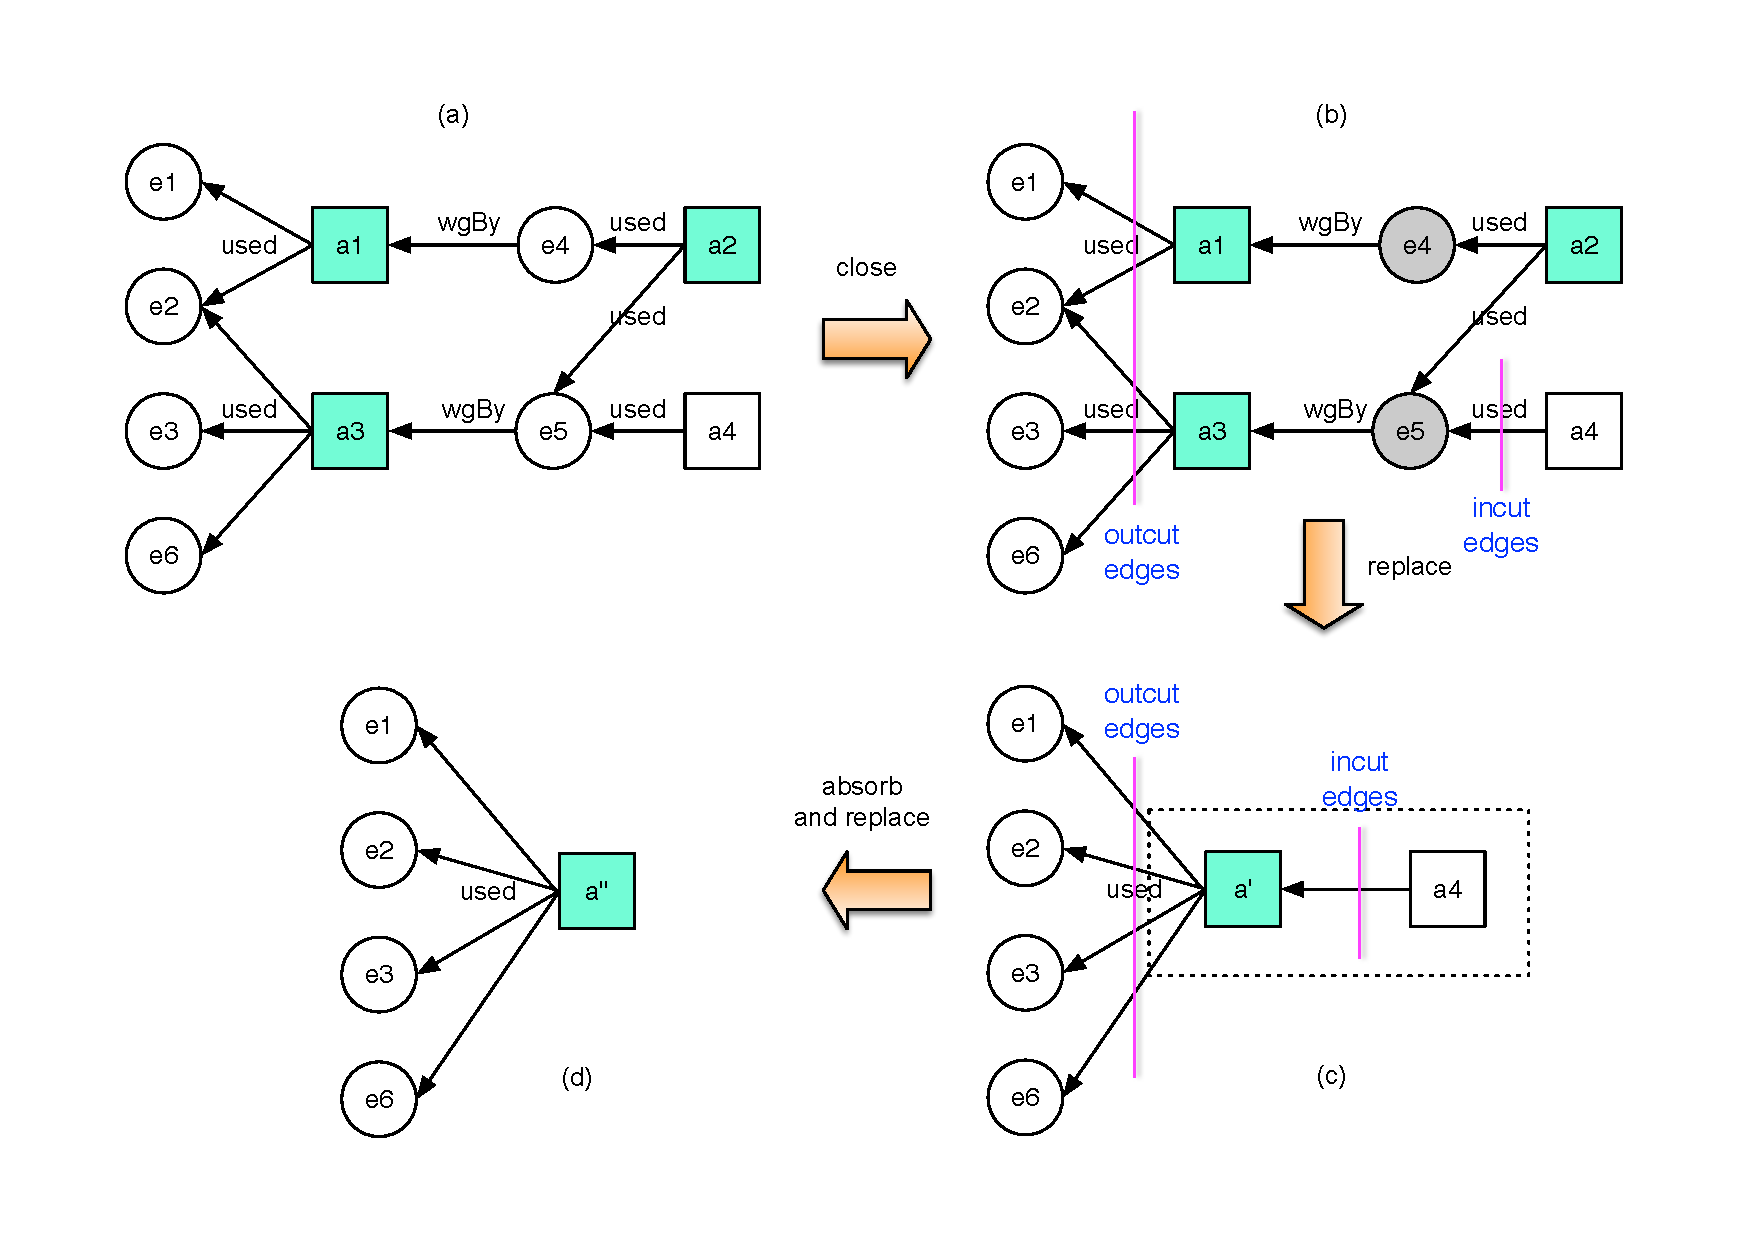
\includegraphics[scale=.5]{figures/convex-a-only-revision.pdf} 
	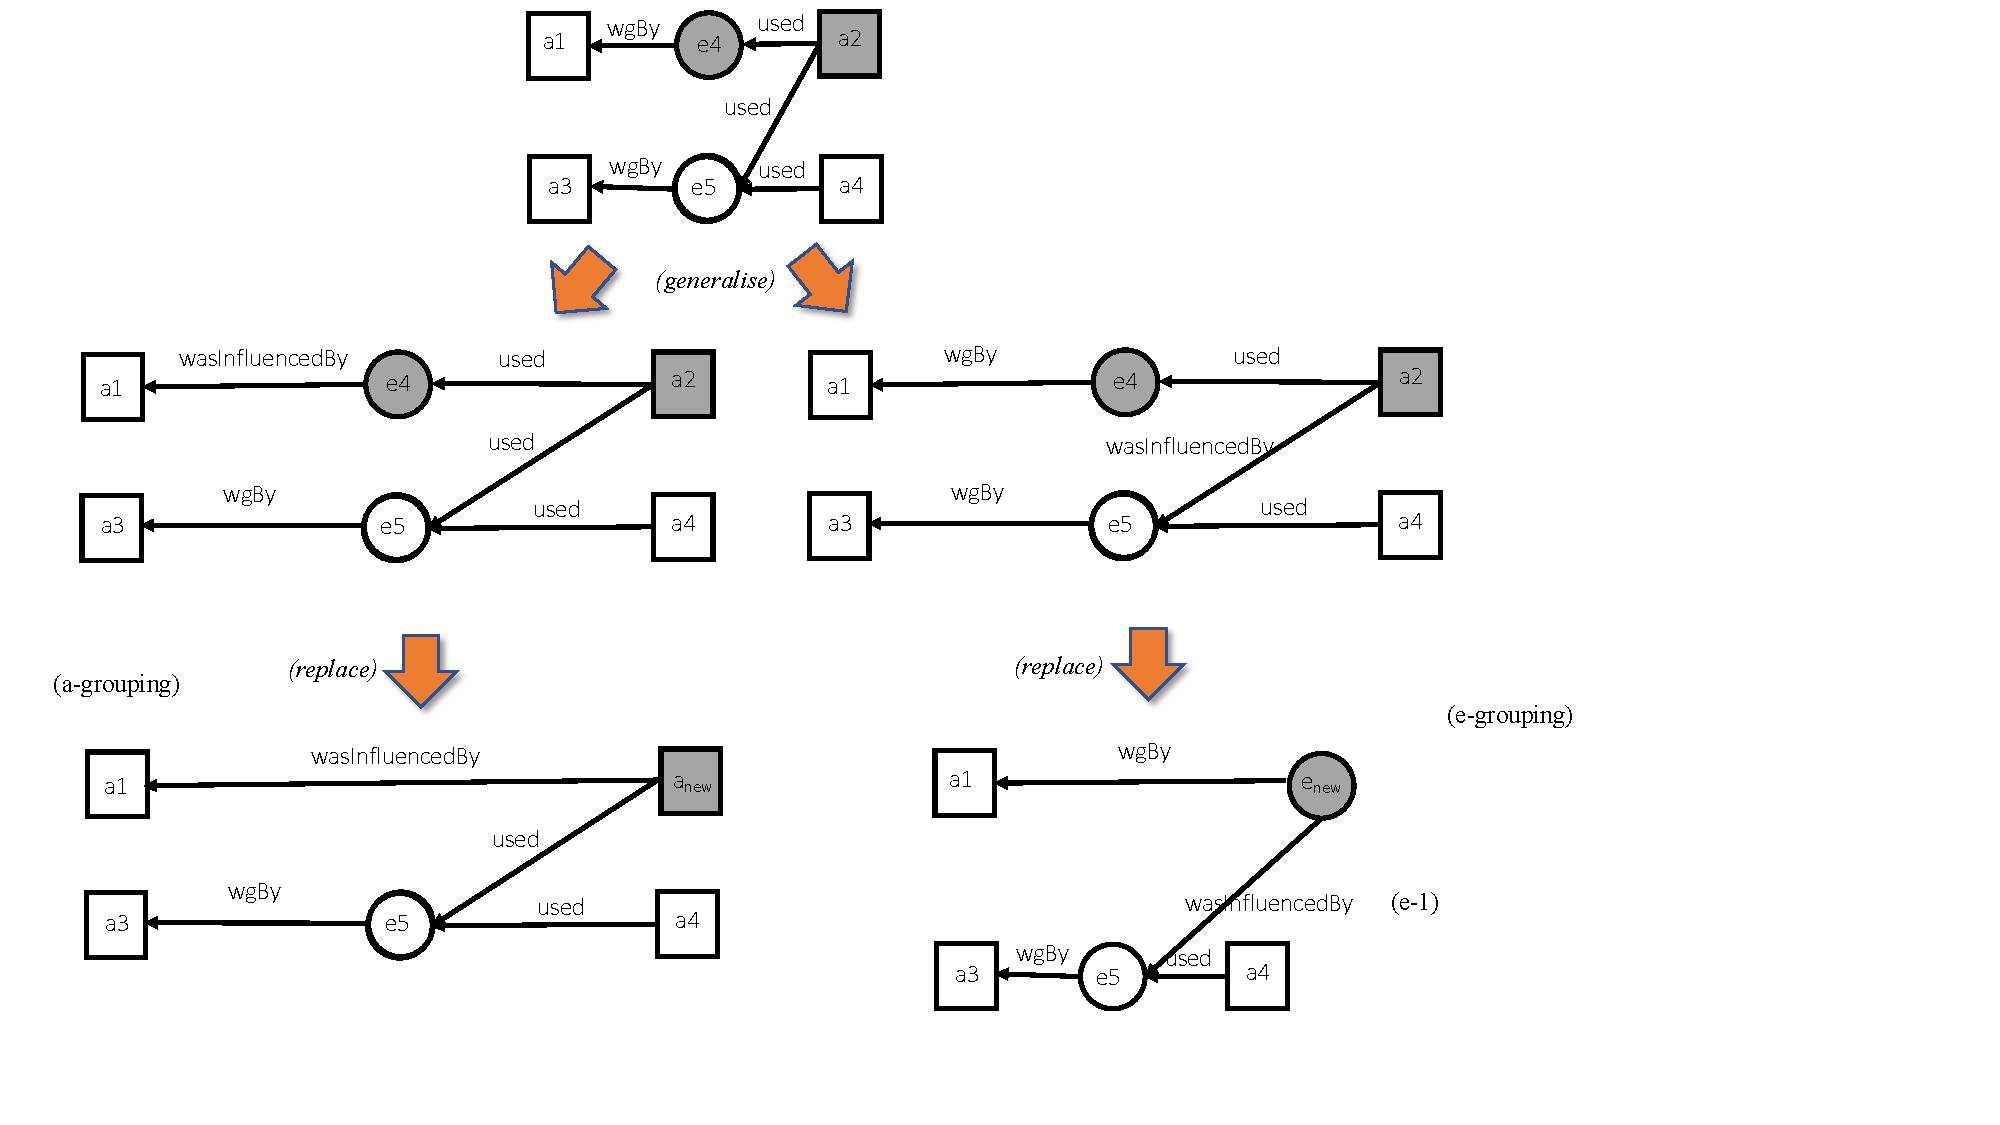
\includegraphics[scale=.5]{wasInfluencedBy-example.pdf} 
	\caption{Abstraction by relationship generalisation} \label{fig:influence}
\end{figure*}


\subsection{Summary}
%\comment{finishing para}
\jwb{We have presented operators that abstract information in a provenance  graph.  We first presented  \emph{homogeneous grouping}  (in Section~\ref{sec:closure}), in which the user selects a set of nodes of the same type, and for which the new, abstract node retains that type. Section~\ref{sec:generalisation} extended this work to allow the user to select any nodes, at the expense of having to chose the type of the final, abstract, node}\jwbtwo{, and gave a further extension to deal with a problem arising from simultaneous generation of events. Section~\ref{sec:justifying} showed that the newly created relations were justified, and Section~\ref{sec:complexity} discussed the complexity of the new operator.}

It is clear that, in order to meet our initial requirement of maintaining type-correctness of the abstracted graph, in general more nodes than just the original ones selected will have to \jwbtwo{be} hidden.
This has implications for the use of this operator, especially given that hidden information may be a critical part of the graph.

\jwbtwo{The choice that we make in this paper is to develop the abstraction operator without paying attention to the risk of removing too much information.}
\jwbtwo{This has the advantage that it allows us to ensure that the operator maintains the PROV-compliance of the new graph, but the disadvantage that the loss of information cannot be controlled.}

\jwbtwo{An alternative} approach is to \jwbtwo{sub-divide} the initial set chosen by the user into multiple smaller sets, thereby reducing the amount of extra information hidden. \jwbtwo{This subdivision could be done manually, at the cost of a greater cognitive load for the user, but ideally would be done automatically, with the algorithm searching for an ``ideal" subdivision according to some optimisation function.} 
\jwbtwo{Care would be required to develop this algorithm. For example the subdivision could be taken to its logical limit by abstracting individual nodes, but this  would have to be balanced  against the increasing revelation of the structure of the graph. Understanding these trade-offs to develop an automatic approach would require substantial testing and evaluation.}  The significance of this trade off would have to be considered in a particular context, and  a full investigation is beyond the scope of this paper.
  


%\jwbtwo{One approach to controlling the loss of information is to sub-divide the initial set of chosen nodes into groups, and to apply the operator to each of these groups in turn. 

\jwbtwo{This approach would also require a measure of evaluating the ``damage'' to a graph caused by an application of an abstraction operator. }
We address \jwbtwo{the issue of damage evaluation}  in~\citep{Missier2014} where we present a simple policy model and language for controlling abstraction, in the context where provenance owners want to control the disclosure of their provenance graphs. There, the owner defines a policy which results in a sensitivity value being associated with nodes, which gives us a means of evaluating the ``damage'' to a graph caused by the abstraction operator.
In~\citep{Missier2014} we do this by means of defining a property \emph{utility} as a counterpart to sensitivity. It is used to indicate  the interest of the provenance owner in ensuring that a node be retained as part of the graph, as it represents important evidence which is not sensitive.   The utility values associated to different nodes are used to quantify any loss of utility as a result of the application of \emph{group} though a measure of \emph{residual utility}. If we write the utility of a node $n$ as $u(n)$, and  $V_{ret} = V / V_{gr}$ is the set of nodes \emph{not} intended to be hidden, and $V'_{ret} \subset V_{ret}$ the nodes which were in fact retained after grouping, the  residual utility is simply
\begin{align}
  RU_{V} = \frac{\Sigma_{n\in V'_{ret}} u(n)}{\Sigma_{n\in V_{ret}} u(n)}
\end{align}
  which is a measure of the proportion of the graph utility not selected by the grouping operator. 



%\comment{Address: It is not evident what is the impact of hiding information which the user did not select, especially information that was obfuscated to maintain validity?  What if the non selected obfuscated content is actually the information that must be communicated between the two parties. }




%%-*- mode: LaTeX; mode: FlySpell; -*-

\section{Abstraction over events}
\label{sec:event}

\begin{figure*}
	\centering
	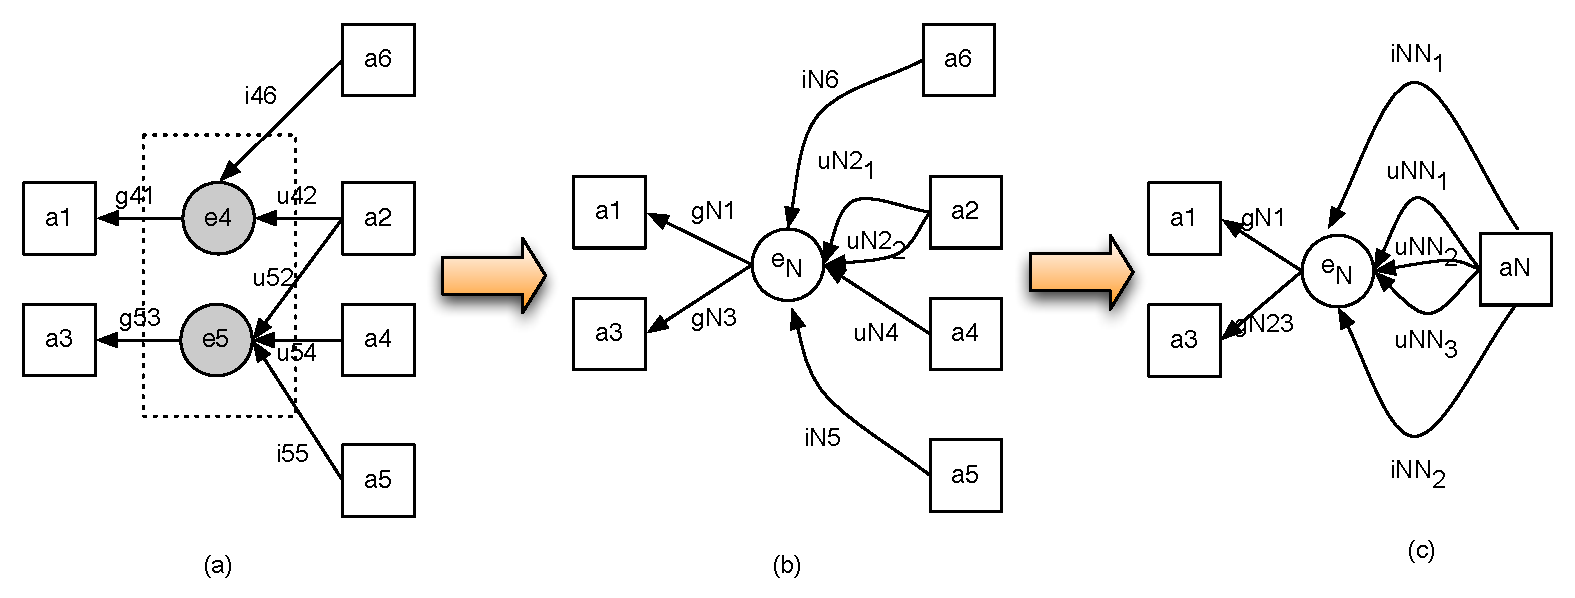
\includegraphics[scale=.5]{figures/e4-e5.pdf} 
	\caption{Abstraction over a document content, and associated abstracted events} \label{fig:e4-e5}
\end{figure*}

In Sec.~\ref{sec:prov-constraints} we recalled the definition of PROV ordering  constraints C2-C7, given in the PROV-CONSTRAINT document, which must be satisfied by any valid PROV graph.
We now want to extend such formal definition of validity to include \textit{abstract} graphs $G'$. 
To achieve this, we must first define suitable events on $G'$. 
When $G'$ is obtained using either e-grouping or a-grouping over some base graph $G$,  in general these are not the same events as $G$'s, because both entities and relationships may have changed. 
Specifically, when $a_{new}$ is created through a-grouping, $G'$s events include 
 $start(a_{new})$, $end(a_{new})$, as well as 
$ev(\used(e, a_{new}))$, $ev(\wgby(a_{new}, e))$ for all $e$ that are generated by or used by $a_{new}$. 
For e-grouping, the new events are $ev(\wgby(e_{new}, a))$ and  $ev(\used(e_{new},a))$ for any $a$ that has generated (resp. used) $e_{new}$.
%
We are going to refer to the two sets of events in $G$ and $G'$ as $EV_{G}$, $EV_{G'}$, respectively.

Note: we have been using symbols like $g_{41}$ in the figure to indicate relationships like $wgby(e_4, a_1)$. 
With slight abuse of notation, but in the interest of simplicity, in the following we are going to use $g_{41}$ to also denote $ev(\wgby(e_4, a_1))$ when it is clear from the context that we refer to the event rather than to the relationship itself.

To fix ideas, consider $G$ in Fig.~\ref{fig:e4-e5}(a), where two sections of a document are independently generated by two editing activities, and then they are independently used by four more activities. Note that this is a slight extension of the abstract pattern of Fig.~\ref{fig:e2-a4}, where the document sections are $e_4$, $e_5$.
%
The e-grouping set $V_{gr} = \{ e_4, e_5\}$ represents the whole document. 

Let $G'$ be the result of (non-strict) e-grouping, as depicted in Fig.~\ref{fig:e4-e5}(b), where the abstract generation and usage events are given new names, namely $g_{Ni}$ as a shorthand for $\wgby(e_N,a_i)$, and $u_{Ni_j}$ for each usage $j$ of the form $\used(a_i, e_N)$. 
Thus, $EV_G = \{ g_{41}, g_{53}, u_{42}, u_{52}, u_{54} \}$ and $EV_{G'} = \{ g_{N1}, g_{N3}, u_{N2_1}, u_{N2_2}, u_{N_4} \}$.
%
If $G$ is valid, the following must hold (constraint C3):
\begin{align}
\label{eq:c3-G}
g_{41} \preorder u_{42}, \quad g_{53} \preorder u_{52}, \quad g_{53} \preorder u_{54} 
\end{align}
where $\preorder$ is the preorder relationship introduced in Sec. ~\ref{sec:prov-events}.

Similarly, for $G'$ to be valid we must have:
\begin{align}
g_{N1} \preorder u_{N2_1}, \quad g_{N1} \preorder u_{N2_2}, \quad g_{N1} \preorder u_{N_4}  \label{eq:c3-global1} \\  
g_{N3} \preorder u_{N2_1}, \quad g_{N3} \preorder u_{N2_2}, \quad g_{N3} \preorder u_{N_4} \label{eq:c3-global2} 
\end{align}

Recall that the PROV-DM recommendation document~\citep{w3c-prov-dm}, defines generation and usage events as follows:
%\begin{description}
\begin{itemize}
	\item\textbf{Generation} \textit{is the completion of production of a new entity by an activity} (Sec. 5.1.3)
	\item\textbf{Usage} \textit{is the beginning of utilizing an entity by an activity} (Sec. 5.1.4)
%	\item\textbf{Invalidation} \textit{is the start of the destruction, cessation, or expiry of an existing entity by an activity. The entity is no longer available for use (or further invalidation) after invalidation. Any generation or usage of an entity precedes its invalidation.} (Sec. 5.1.8)
\end{itemize}

Thus, $e_{N}$ is generated when both generation events $g_{N1}, g_{N3}$ have occurred (incidentally, this implies that these abstract events must be simultaneous), and it start being used when the ``earliest'' of the usage events takes place, keeping in mind that no ordering relationships amongst the usage events is necessarily defined.

Intuitively, it should be possible to map abstract events to corresponding  original events in $G$, in such a way that validity of $G'$ follows from the validity of $G$.
%
To formalise this idea, we propose to define the  events in $EV_{G'}$ in terms of events in $EV_{G}$, that is, by means of a function $\psi$ that maps each $ev' \in EV_{G'}$ to a corresponding event in $EV_{G}$:
\begin{align}
 \psi: EV_{G'} \rightarrow EV_{G} 
\end{align}
Furthermore, we want $\psi$ to be order-preserving, so that the validity of $G'$ relative to temporal constraints can be derived from the validity of $G$ using $\psi$: 
\begin{align}
 ev_1' \preorder ev_2' \Rightarrow \psi(ev_1') \preorder \psi(ev_2')  
\end{align}
where the same preorder $\preorder$ is used for both sets (because that is defined by the constraints).

We now look for a suitable mapping $\psi$. Consider for instance:
\begin{equation}
\psi(g_{N1}) = g_{41} ,  \quad  \psi(g_{N3}) =  g_{53},  \quad   \psi(u_{N2_1}) = u_{42}  \quad \psi(u_{N2_2}) = u_{52} \quad \psi(u_{N4}) = u_{54} \label{eq:psi-zero}
\end{equation}
This is a ``natural'' mapping, which follows the mapping between abstract and original relationships induced by the grouping operator.
Since $\psi$ is order-preserving, from (\ref{eq:psi-zero}) and (\ref{eq:c3-global2}), it follows that:
\begin{equation}
  g_{41} \preorder   u_{52}, \quad  g_{53} \preorder   u_{42}
  \label{eq:over-constraints}
  \end{equation}
However, we observe that neither of these relationships hold on $EV_G$, in fact the ordering of $g_{41}$ (resp $g_{53}$) relative to $u_{52}$ (resp $u_{42}$) is undefined.
Thus, if we consider all the possible total orderings in $EV_G$ that are consistent with $\preorder$, we see that this choice of mapping function restricts the possible interpretations of $EV_{G'}$, when we assume that $G'$ is valid, to only a subset of these orderings, namely those where the additional relationships (\ref{eq:over-constraints}) also hold.

We use this example to motivate a broader definition of $\psi$ that does not incur such restriction. For this, we first redefine $\psi$ to map each event in $EV_{G'}$ to a \textit{set} of events in $EV_{G}$:
\begin{align}
 \psi': EV_{G'} \rightarrow {\cal P}(EV_{G}) 
\end{align}
(where ${\cal P}(EV_{G})$ denotes a powerset).
%
Then, we introduce a new preorder $\preorderprime$ on ${\cal P}(EV_{G})$, such that:
\begin{align}
 S_1 \preorderprime S_2 \text{ iff for each } s_1 \in S_1, \exists s_2 \in S_2 \text{ such that } s_1 \preorder s_2 
 \end{align}
We can now define mapping $\psi'$ that is order-preserving:
\begin{align} 
ev_1' \preorder ev_2' \Rightarrow \psi(ev_1') \preorderprime \psi(ev_2')  
\end{align}
as follows:
\begin{equation}
\psi(g_{N1}) = \{ g_{41}, g_{53} \},  \quad  \psi(u_{N2_1}) =  \psi(u_{N2_4}) = \{ u_{42}, u_{52} \}, \quad \psi(u_{N4}) = \{u_{54} \} \label{eq:psi-real}
\end{equation}
It is easy to see for example that, with this mapping, the constraints 
$g_{N1} \preorder u_{N2_1}$, $g_{N3} \preorder u_{N2_2}$ both imply $ \{ g_{41}, g_{53} \} \preorderprime  \{ u_{42}, u_{52} \} $,
which includes interpretations on $G$ where the new constraints (\ref{eq:over-constraints}) need not hold.
The specification of $\psi'$ follows easily from the computation of the grouping operator, and details are omitted.

In summary, we have proposed to introduce (i) a set of abstract events on $G'$ so we can verify its validity relative to temporal constraints, (ii) a mapping function that defines abstract events in terms of original events in $G$, and (iii) a set-based preorder such that the mapping can be order-preserving without imposing additional constraints on $G$. 


%%OBSOLETE. retrieve from git is we change our minds.
%\subsection{Mappings for abstract events }
%
%The following questions provide a useful starting point for reasoning about events. Firstly, given the generation events $g_{41}$, $g_{53}$  of each of the document sections, when was the entire document $e_N$ generated? 
%%
%When did $a_2, a_4$ use the document? 
%%
%Secondly,  suppose after the first grouping one performs two additional a-groupings, first with $V_{gr} = \{a_1, a_3\}$, and then with $V_{gr} = \{a_2, a_4, a_5, a_6\}$.
%%
% This results in the abstraction depicted in Fig.~\ref{fig:e4-e5}(c), which reads simply ``(abstract) document $e_N$ was used by (abstract) activity $a_N$''. 
% In this abstraction, what happens to the original generation and usage events?
%
%Initial help in answering these questions comes from the PROV-DM recommendation document~\citep{w3c-prov-dm}, namely:
%%\begin{description}
%\begin{itemize}
%\item\textbf{Generation} \textit{is the completion of production of a new entity by an activity} (Sec. 5.1.3)
%\item\textbf{Usage} \textit{is the beginning of utilizing an entity by an activity} (Sec. 5.1.4)
%\item\textbf{Invalidation} \textit{is the start of the destruction, cessation, or expiry of an existing entity by an activity. The entity is no longer available for use (or further invalidation) after invalidation. Any generation or usage of an entity precedes its invalidation.} (Sec. 5.1.8)
%\end{itemize}
%%\end{description}
%
%%
%Let us consider these definitions in the context of our example. Firstly, the generation of the whole document is only complete upon generation of the last section. Thus, each of the generation events of $e_N$, denoted $g_{N1}$ and $g_{N3}$ in Fig.~\ref{fig:e4-e5}(b), cannot precede $g_{41}$, $g_{53}$. This can be written as the ordering constraints:
%\begin{align}
% \label{eq:gprime-order1}
%max\{g_{41}, g_{53}\} \leq g_{N1} \\
%max\{g_{41}, g_{53}\}  \leq g_{N3}
%\end{align}
%Furthermore, we know from constraint C2 that $g_{N1}$ and $g_{N3}$ must be simultaneous:
%$g_{N1} = g_{N3}$.
%
%
%Secondly, symmetrically to generation, usage of the document ($u_{N2_1}, u_{N2_2}, u_{N4}$) in Fig.~\ref{fig:e4-e5}(b) begins with the earliest usage by any of the consuming activities:
%\begin{align}
%u_{N2_1} \leq u_{42} \label{eq:gen-usage1}\\
%u_{N2_2} \leq u_{52}  \label{eq:gen-usage2}\\
%u_{N4} \leq u_{54}  \label{eq:gen-usage3}
%\end{align}
%%
%Finally, from the definition above, the rule for invalidation follows the same pattern as usage:
%%
%\begin{align}
%i_{N6} &\leq i_{46} \label{eq:inv1}\\
%i_{N5} &\leq i_{55}  \label{eq:inv2}
%\end{align}
%%
%Furthermore, C3 requires each generation to precede each usage:
%%
%\begin{align}
%g_{N1} &= g_{N13}  \leq  u_{N2_1}  \quad  \\
%g_{N1} &= g_{N13}  \leq  u_{N2_2}  \quad  \\
%g_{N1} &= g_{N13}  \leq  u_{N4}  \label{eq:gprime-order2}
%\end{align}
%%
%and C4, C5 require both generation and usage to precede invalidation:
%%
%\begin{align}
%g_{N1} &= g_{N3} \leq i_{N6}  \quad g_{N1} = g_{N3} \leq i_{N5} \\
%u_{N2_1} &\leq i_{N6}  \quad u_{N2_1} \leq i_{N5} \\
%u_{N2_2} &\leq i_{N6}  \quad u_{N2_2} \leq i_{N5} \label{eq:inv-last}
%\end{align}
%%
%In order to avoid excessive clutter in the example, start and generation constraints are only discussed in the next section, along with all general ordering constraints on $G'$.
%
%
%Now, consider the  linear orderings in $G$ under the assumption that \textit{every generation event precedes every usage event} and \textit{every usage event precedes every invalidation event}, that is, there is a ``generation phase'' followed by a ``usage phase'' and by an ``invalidation phase'' (Fig.~\ref{fig:e-grouping-orderings}(a)). It is easy to see that, with this assumption, all these orderings are consistent with constraints (\ref{eq:gprime-order1}) through (\ref{eq:inv-last}), provided that we redefine $G'$ events to be \textit{simultaneous} to corresponding $G$ events, as follows:
%
%\begin{figure*}
%\centering
%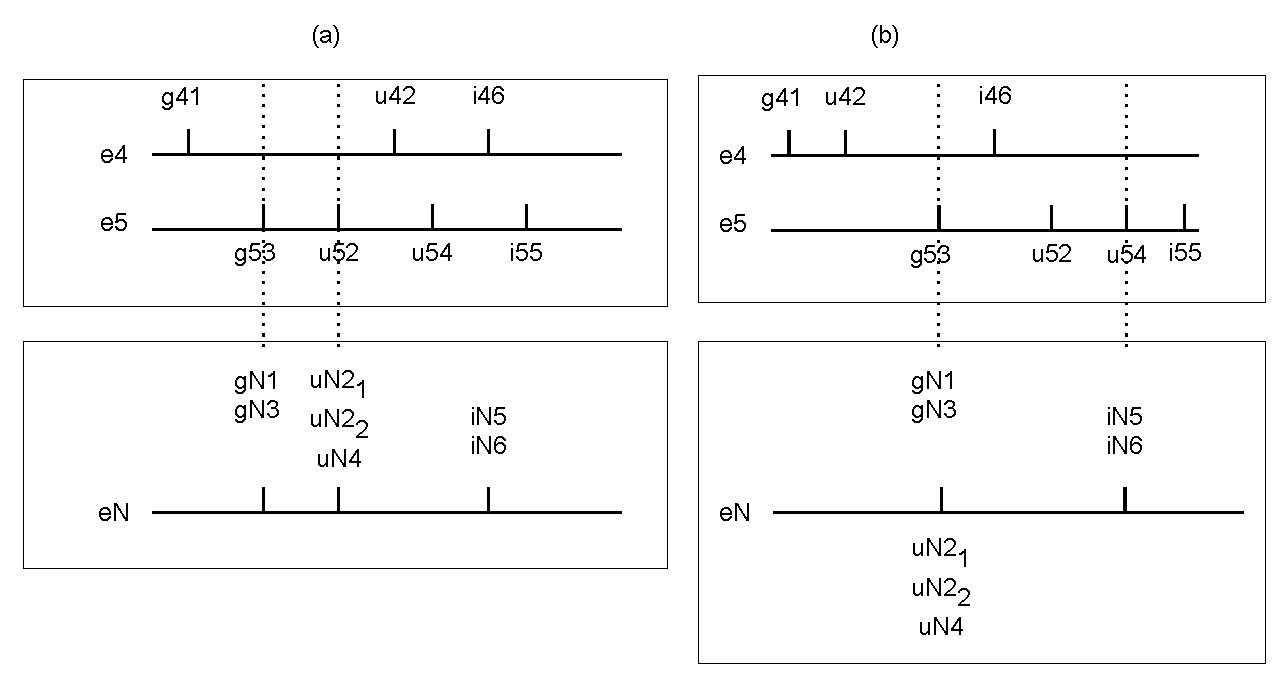
\includegraphics[scale=.5]{figures/e-grouping-orderings.pdf} 
%\caption{Two possible orderings on $G$ (top), and corresponding orderings on $G'$ (bottom)} \label{fig:e-grouping-orderings}
%\end{figure*}
%
%
%\begin{align}
%g_{N1} = g_{N3} = max\{g_{41}, g_{53}\}   \label{eq:max} \\
%u_{N2_1} = u_{N2_2}  = u_{N4} = min\{u_{42},  u_{52},  u_{54}\}   \label{eq:usage-min-simple} \\
%i_{N5} = i_{N6}  = min \{   i_{46},  i_{55} \}   \label{eq:inval-min-simple}
%\end{align}
%In this case we conclude that $G'$ is valid by our assumption that each of its generation events precedes each of its usage events.
%
%Consider now the more general case where generation, usage and invalidation events are interleaved for different entities in $V_{gr}$. Fig.~\ref{fig:e-grouping-orderings}(b) shows such an interleaving for our example. In this case, 
%$min \{   u_{42},  u_{52},  u_{54} \} = u_{42} \leq g_{53} = max\{g_{41}, g_{53}\}$.
%%
%This violates (\ref{eq:gen-usage1}) through (\ref{eq:gen-usage3}).  In other words, this more general family of interpretations over $G$ is not represented in $G'$ when the abstract events in $G'$ are defined using the inequalities above. 
%
%In order to account for this general case, we modify  (\ref{eq:usage-min-simple}) and (\ref{eq:inval-min-simple}) as follows:
%\begin{align}
%u_{N2_1} &= u_{N2_2}  = u_{N4} = max\{ g_{41}, g_{53}, min \{u_{42},  u_{52},  u_{54}\}\}  \label{eq:usage-min} \\
%i_{N5} &= i_{N6}  = max\{g_{41}, g_{53}, u_{42},  u_{52},  u_{54}, min\{i_{46},  i_{55}\}\}   \label{eq:inval-min}
%\end{align}
%%
%
%In the example of Fig.~\ref{fig:e-grouping-orderings}(b), this stricter constraint results in  generation and usage events in $G'$ to all be simultaneous to $g_{53}$, while the invalidation events are shifted later in the event line, to the latest usage. Note that in the special case of Fig.~\ref{fig:e-grouping-orderings} (a), constraints (\ref{eq:usage-min-simple}), (\ref{eq:usage-min}) and (\ref{eq:inval-min-simple}), (\ref{eq:inval-min})  are pairwise equivalent.
%
%The reasoning used in the examples just presented justifies the following definitions for the general inequalities which define abstract events in terms of events in $G$.
%
%\subsection{Abstract events for e-grouping}
%\label{sec:abstract-events-for-e-grouping}
%%
%Let $G=(V,E) \in \guEA$, $V_{gr} \subset V$ be the set of nodes that are to be grouped, and  $e_{new} \in \en$ be the new entity node introduced through e-grouping as per Def.~\ref{eq:t-grouping}.
%% 
%
%\paragraph*{\textbf{Abstract Generation events}}
%Let $V^*$ to denote $\extend(\clos(V_{gr},G), \en)$, and let $\wgby_{out}$ denote the set of generation relations involving entity nodes in the extension
%$V^*$, and activity nodes outside of the extension:
%\begin{align*} 
%\wgby_{out} = \{ \wgby(e,a) |  e \in V^*,  a \notin V^* \}
%\end{align*} 
%In the example of Fig.~\ref{fig:e4-e5}, $\wgby_{out} = \{ g_{41}, g_{53} \}$.
%
%%
%Correspondingly, let $\wgby'_{out}$ denote the generation relations that involve $e_{new}$:
%\begin{align*} 
%\wgby'_{out} = \{ \wgby(e_{new},a) | a \notin V^* \}
%\end{align*} 
%In the example, $\wgby'_{out} = \{ g_{N1}, g_{N3} \}$.
%
%In general, we will denote values in the abstracted prov graph by primed versions of their counterparts in the original graph. The exception to this will be relationships and events involving $e_{new}$, since $e_{new}$ is  a new entity that does not appear in the old graph.
%
%The following equalities, define the orderings of the events associated with the relations in $\wgby'_{out}$.
%
%
%\vspace*{10pt}
%\begin{definition}[Abstract generation events - e-grouping]
%\label{def:abstract-gen-e}
%
%\paolotwo{Replace max with a new event that dominates all of the $ev(g)$ and adjust the def below accordingly}
%
%For each $g' \in \wgby'_{out}$:
%\[
%ev(g') = max \{ ev(g) | g \in \wgby_{out} \}  
%\]
%For all activities $a$ that participate in generating the new event $e_{new}$, we set the generation event to
%\[
%ev(\wgby(e_{new},a)) = max \{ ev(g) | g \in \wgby_{out} \}
%\]
%\end{definition}
%
%%\vspace*{10pt}
%%\begin{definition}[Abstract usage events - e-grouping] 
%%\label{def:abstract-usage-e}
%%Let
%%\[u'_{min} = min_{ u \in \used_{in} } ( ev(u) \}\] and let 
%%$g'_{max} = max_{g \in \wgby_{out}} ( ev(g) \} $.\\
%%For each $u' \in \used'_{in}$:
%%\begin{equation}
%%v(u') = max \{ g'_{max} , u'_{min} \}
%%\end{equation}
%%\end{definition}
%
%\paragraph*{\textbf{Abstract Usage events}}
%Usage events for e-grouping are defined similarly by generalization from (\ref{eq:usage-min}), as follows.
%%
%Let $\used_{in}$ denote the set of usage relations involving entity nodes in the extension
%$V^*$, and activity nodes outside of the extension:
%\begin{align*} 
%\used_{in} = \{ \used(a,e) |  e \in V^*,  a \notin V^* \}
%\end{align*} 
%In the example of Fig.~\ref{fig:e4-e5}, $\used_{in} = \{ u_{42}, u_{52}, u_{54} \}$.
%
%%
%Correspondingly, let 
%$\used'_{in}$ denote the usage relations that involve $e_{new}$:
%\begin{align*} 
%\used'_{in} = \{ \used(a, e_{new}) | a \notin V^* \}
%\end{align*} 
%In the example, $\used'_{in} = \{ u_{N2_1}, u_{N2_2}, u_{N4}  \}$.
%
%The following equalities, which generalise (15), define the events associated with the relations in $\used'_{in}$.
%
%\vspace*{10pt}
%\begin{definition}[Abstract usage events - e-grouping] 
%\label{def:abstract-usage-e}
%
%
%\paolotwo{min does not always exist so as for max, we need to introduce a new $u$ that is $\leq$ than all of the usage events, and adjust the def below accordingly}
%Let
%\[u'_{min} = min \{ ev(u) | u \in \used_{in} \}\] and let 
%$g'_{max} = max \{ ev(g) | g \in \wgby_{out}\} $.\\
%For each $u' \in \used'_{in}$:
%\begin{equation*}
%ev(u') = max \{ g'_{max} , u'_{min} \}
%\end{equation*}
%and so
%\begin{equation}
%ev(\used(a,e_{new})) = max \{ g'_{max} , u'_{min} \}
%\end{equation}
%\end{definition}
%
%\paolotwo{remove invalidation altogether}
%\paragraph*{\textbf{Abstract Invalidation events}}
%The events equalities for invalidation, exemplified in (\ref{eq:inval-min}), follow the pattern used above for usage. The only difference is that $\used'_{in}$ is replaced by 
%\[ \inv'_{in} = \{ \inv(a, e_{new}) | a \notin V^* \} \]
%In our example, $ \inv_{in} = (  i_{46}, i_{55} \}$,  $\inv'_{in} = ( i_{N6}, i_{N5} \}$.
%%
%The corresponding definition is as follows.
%
%\vspace*{10pt}
%\begin{definition}[Abstract invalidation events] 
%\label{def:abstract-inv}
%Let
%\[i'_{min} = min \{ ev(i) | i \in \inv_{in} \}\]
%and 
%\[u'_{max} = max \{ ev(u) | u \in \used_{in} \}\]
%For each $i' \in \inv'_{in}$:
%\[
%ev(i') = max \{ g'_{max} , u'_{max},  i'_{min}\}
%\]
%and thus for each activity $a$  that participates in the invalidation of $e_{new}$, invalidation is the latest of the new generation event $g'_{max}$, the latest usage event $u'_{max}$ and the minimum of the original invalidation events.  
%\begin{equation}
%\inv(a,e_{new}) = max \{ g'_{max} , u'_{max},  i'_{min} \}
%\end{equation}
%\end{definition}
%
%
%{\bf Start events:} Now that the event of usage and generation of $e_{new}$ has been fixed, we need to ensure that the activities involved in these events continue to meet the constraints that apply to them. This includes start and end events for activities related to our new entity $e_{new}$ by either $\wgby$ or $\used$.  
%
%
%%In addition, a-grouping also produces new abstract start and end events for the new activity $a_{new}$. 
%% The situation is illustrated in the timelines of Fig.~\ref{fig:a1-a2}. The right side of figure (a) shows a possible interleaving of events in $G$, which is consistent with constraints C2-C7. Intuitively, the start (resp. end) event for the abstract activity $a_N$ cannot follow (resp. precede) the earliest (resp., latest) usage/generation event associated with $a_1, a_2$.
%% %
%% Similar to the case for e-grouping,
%We appeal to the informal definitions of start and end in~\citep{w3c-prov-dm} to derive inequalities for the abstract start and end events for our new activity $a_{new}$.
%% 
%\begin{itemize}
%\item \textbf{Start} \textit{is when an activity is deemed to have been started by an entity, known as trigger. The activity did not exist before its start. Any usage, generation, or invalidation involving an activity follows the activity's start} (See~\citep{w3c-prov-dm},  Section 5.1.6)
%
%\item \textbf{End} \textit{is when an activity is deemed to have been ended by an entity, known as trigger. The activity no longer exists after its end. Any usage, generation, or invalidation involving an activity precedes the activity's end} (See~\citep{w3c-prov-dm}, Section 5.1.7)
%\end{itemize}
%(For simplicity we are going to leave the trigger entity implicit, and simply refer to the start and end events as $\start(a)$ and $\ed(a)$).
%
%\paolotwo{do not think we need (27) because it is implied by the mapping for the abstract generation events. probably (28) not needed either }
%\begin{definition}[Start events - e-grouping] 
%\label{def:abstract-start-e}
%Consider events $a$ such that $\wgby(e_{new},a)$. For each such $a$, we set the new start event $\start'(a)$ as the lesser of the original start event and the generation event $ev(\wgby(e_{new},a))$. Thus
%\begin{equation}
%\start'(a) = min\{\start(a),ev(\wgby(e_{new},a))\}
%\end{equation}
%\end{definition}
%
%{\bf End events:} For all activities $a$ that use the newly created entity, we must ensure that ensure that the end of the activity does not precede any $\used(a,e_{new})$ events.
%\begin{definition}[End events - e-grouping]
%  \label{def:abstract-end-e}
%  If the set of all usage events by $a$ of $e_{new}$ is denoted $\{ev(\used(a,e_{new}))\}$, we set the new end events $\ed'(a)$ to be
%  \begin{equation}
%  \ed'(a) = max\{\ed(a), max\{ev(\used(a,e_{new}))\}\}
%\end{equation}
%\end{definition}
%
%A proof of that, given the definitions above, the  constraints of Section~\ref{sec:prov-constraints} are satisfiable, is given in~\ref{sec:consistency-constraints-e-grouping}.
%
%
%\subsection{Abstract events for a-grouping}
%\label{sec:abstract-events-for-a-grouping}
%% \begin{figure}
%% \centering
%% 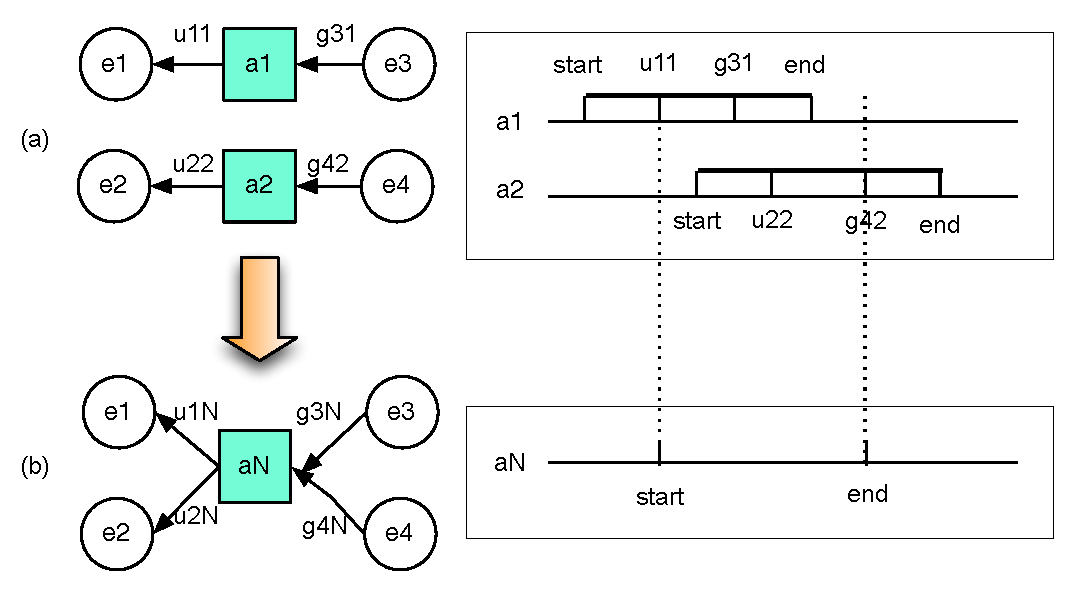
\includegraphics[scale=.5]{figures/a1-a2.pdf} 
%% \caption{Abstraction for start/end events} \label{fig:a1-a2}
%% \end{figure}
%
%Generation and usage abstract events follow a very similar pattern as those for e-grouping, except that the new node introduced by grouping is an activity node: $a_{new} \in \act$.
%%
%%This is illustrated in Fig.~\ref{fig:a1-a2}.
%As a consequence, the abstract event definitions given in the previous section also follow the same pattern, but with the roles of entities and activities reversed. They are summarized here below.  We now use $V^*$ to mean the group of nodes collected by $\extend(\clos(V_{gr},G), \act)$.
%
%%\jwb{I (personally) find the notations below confusing, and would rather get rid of them. I haven't used them much in the rest of this section.}
%%
%%\begin{align*} 
%%\wgby_{in} & =  \{ \wgby(e,a) |  e \notin V^*, a \in V^* \} \\
%%\wgby'_{in} &  = \{ \wgby(e, a_{new}) | e \notin V^* \} \\
%%\used_{out} & = \{ \used(a,e) |  e \notin V^*,  a \in V^* \} \\
%%\used'_{out} & = \{ \used(a_{new}, e) | e \notin V^* \}
%%\end{align*} 
%%
%%
%%
%
%\paolotwo{def 14 makes no sense as we again need to introduce artificial min and max to account for the abstract start and end events}
%The new start (resp. end) event is taken to be the minimum (resp. maximum) relevant start (resp. end)  event.
%\begin{definition}[Abstract start and end events - a-grouping] 
%\label{def:abstract-start-and-end-a}
%\begin{align*}
%  \start(a_{new}) & = min\{\start(a) | a \in V^*\} \\
%  \ed(a_{new}) & = max\{\ed(a) | a \in V^*\} \\
%\end{align*}
%\end{definition}
%
%\begin{definition}[Abstract generation events - a-grouping]
%\label{def:abstract-gen-a}
%%Since generation events must be simultaneous, we can assume that they are simultaneous in the original graph. 
%%
%%For any entity $e$ not in $V^*$ that is generated by an activity $a$ in $V^*$, the new generation event cannot be before the start of the abstracted activity $a_{new}$, taken as the minimum of the original start events s in Definition~\ref{def:abstract-start-and-end-a}. However,
%Constraint C2 applies to the original graph, so for all activities $a,b$ that participate in the generation of $e$, $ev(\wgby(e,a)) = ev(\wgby(e,b))$. 
%
%
%%\jwb{Should we do start and end definitions first? Start and end only apply to ctivities, so the definition below already excludes entities}
%The new generation event is thus given as
%%  \begin{align*}
%%   ev(\wgby(e,a_{new})) =  max\{ &  \start(a_{new}), \\ 
%%                                & min\{ev(\wgby(e,a))  | a \in V^*\} \}
%% \end{align*}
%  \begin{align*}
%   ev(\wgby(e,a_{new})) =  ev(\wgby(e,a))
% \end{align*}
%
%\end{definition}
%
%\vspace*{10pt}
%\begin{definition}[Abstract usage events - a-grouping] 
%\label{def:abstract-usage-a}
%For an entity $e$ not in $V^*$ which is used by an activity $a$ in $V^*$, the assigned usage event for $a_{new}$ ($ev(\used(a_{new},e))$) is given by  
%\begin{align*}
%ev(\used(a_{new},e)) = max\{ & \start(a_{new}) , \\
%                            & min\{ev(\used(a,e))) | a \in V^*\}\}
%\end{align*}
%\end{definition}
%
%
%\vspace*{10pt}
%\begin{definition}[Abstract invalidation events - a-grouping] 
%  \label{def:abstract-inv-a}
%  By Constraint C8, invalidation events from two distinct activities are simultaneous.
% %
%For an entity $e$ which is invalidated by an activity $a$ in $V^*$, the event of the invalidation event remains the same when the activity is abstracted.
%\[
%ev(\inv(a_{new},e)) = min\{ev(\inv(a,e)) | a \in V^*\}
%\]
%\end{definition}
%
%A proof of that, given the definitions above, the  constraints of Section~\ref{sec:prov-constraints} are satisfiable, is given in~\ref{sec:consistency-constraints-e-grouping}.




%%-*- mode: LaTeX; mode: FlySpell; -*-

\section{Abstraction with Agents}  \label{sec:agents-abstraction}

Having laid the foundations for abstraction on the core $\guEA$ model, extending grouping to a model that also includes agents, the third pillar of the PROV model, is quite straightforward. Agents may be humans or software systems. 
%
Specifically, we now consider the node type $\ag$ and the following additional relation types from the PROV schema of Sec.~\ref{sec:prov-core}:

\begin{eqnarray*}
\waw      & \subseteq & \act \times \ag \\
\attrTo   & \subseteq & \en \times \ag \\
\delegate & \subseteq & \ag \times \ag  
\end{eqnarray*}
% \begin{align*}
% \waw \subseteq \act \times \ag \\
% \attrTo \subseteq \en \times \ag \\
% \delegate \subseteq \ag \times \ag  
% \end{align*}
% %Instances of this extended model now include the three relation types above.
%$\{\attrTo(e,ag)|e \in \en, ag \in \ag\} \cup \{\waw(a,ag)|a \in \act, ag \in \ag\} \cup \{ \delegate(ag_1, ag_2) | ag_1, ag_2 \in \ag\}$. 
%

We use the shorthand relation names $\waw$,  $\attrTo$ and $\delegate$  for \textit{wasAssociatedWith},  \textit{wasAttributedTo} and \textit{actedOnBehalfOf}. These denote responsibility of an agent for an activity ($\waw$), responsibility of an agent for an entity ($\attrTo$), and delegation between two agents ($\delegate$). 
%

Note that PROV admits an additional optional activity element to $\delegate$, which is used to  qualify the delegation as occurring within the scope of that activity. For simplicity, we are not going to consider this qualified version of the relation.
%
Thus, we can still assume that these new relations are binary, and so we continue to view an instance of a provenance graph as a directed graph $G=(V,E)$, where new $V= \en ~\cup~ \act ~\cup~ \ag$, and where each relation instance maps to a labelled directed edge.  We denote the set of all such graphs as $\guaEAG$.

The main implications of adding agents to our abstraction model are that (i) a new \textit{ag-grouping} operator must be introduced, and (ii) the existing definitions of e-grouping and a-grouping must be modified slightly. 

In order to incorporate agents into the definition of $\group$, observe that, for all three relations involving agents, the agent node is always the \textit{target} of the directed edge.
%
This means that agents can be viewed as part of an ``outer layer'' in the provenance graph.
%
This is illustrated in Fig.~\ref{fig:agents-baseline}, where the agent nodes and new relations are shown in bold lines in the outer side of the digraph.

\begin{figure}
\centering
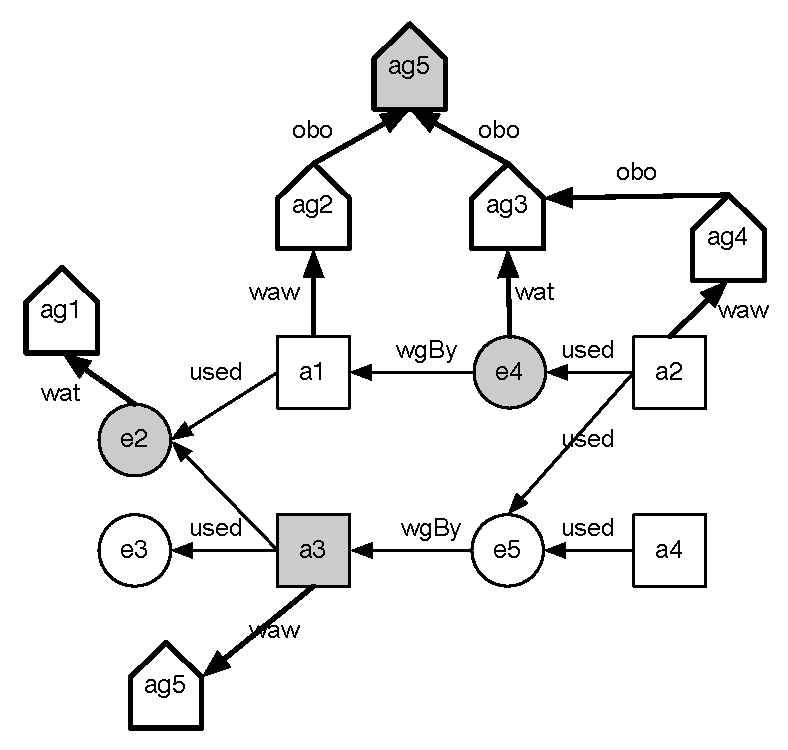
\includegraphics[scale=.5]{figures/agents-baseline}
\caption{$\guaEAG$ provenance graph. Agents lie on the outer border of the digraph. Shaded nodes show a possible grouping set in the general case.}  \label{fig:agents-baseline}
\end{figure}

This observation suggests we can break down the analysis of grouping with agents into the following three parts.
%
\begin{enumerate}
\item $V_{gr} \subset \ag$. This is the case for ag-grouping, which only involves the outer layer of the graph. Since agents are only related to each other through delegation: $\delegate(ag_1 , ag_2)$, grouping in this case is akin to \textit{homogeneous grouping} from Sec.~\ref{sec:closure}, i.e., no nodes of other types are ever involved, and $v_{new} \in \ag$.

\item $V_{gr} \subset \en \cup \act$ as in Sec.~\ref{sec:grouping}. This is the case of t-grouping (Def.~\ref{def:t-grouping}), where the nodes involved in the abstraction are in the inner layer, but they may be related to agent nodes via $\waw$ and $\wat$ relations.

\item $V_{gr} \subset \en \cup \act \cup \ag$.  Here, the group set may contain any combination of nodes. However, the peripheral role played by agents relative to entities and activities suggests that it may be reasonable to restrict this case to e-grouping or a-grouping, i.e., a combination of node types may include agents, but it should not be abstracted by a new agent node.
%
\end{enumerate}



\subsection{Ag-grouping: abstracting agents}  \label{sec:ag-grouping}

We begin with the case where abstraction is performed over a set of agents, i.e., $V_{gr} \subset \ag$.
%
In this case, the existing definition of t-grouping (Def.~\ref{eq:t-grouping}) extends naturally to $\guaEAG$ graphs.
%
%
T-grouping involves three operators: $\clos$, $\extend$, and $\repl$.
%
Since $\clos(V_{gr}, V)$ operates only on $\delegate$ relations, it follows that its result is also homogeneous, i.e., $\clos(V_{gr}, V) \subset \ag$. Also, there is no need to restore type validity by extending the closure, i.e., $\extend$ is the identity: $\extend(\clos(V_{gr}, V), V, \ag) = \clos(V_{gr}, V)$.
%
Finally, it is easy to see that our original definition of group replace (Def.~\ref{def:group-replace}) is general enough to accommodate the ``rewiring'' of the new abstract agent node. 
%
We illustrate this informally using the patterns of Fig.~\ref{fig:d-chains-abstracted}.
%

In pattern (a), $V_{gr} = \{ ag_1, ag_4 \}$, and $\clos(V_{gr}, V) =  \{ ag_1, ag_2, ag_3, ag_4 \}$.
%
In this case, the closure includes all the intermediate agents in the delegation chain between $ag_1$ and $ag_4$.
%
Replacement trivially transforms $G$ into the single abstract agent $ag_N$.


\begin{figure}
\centering
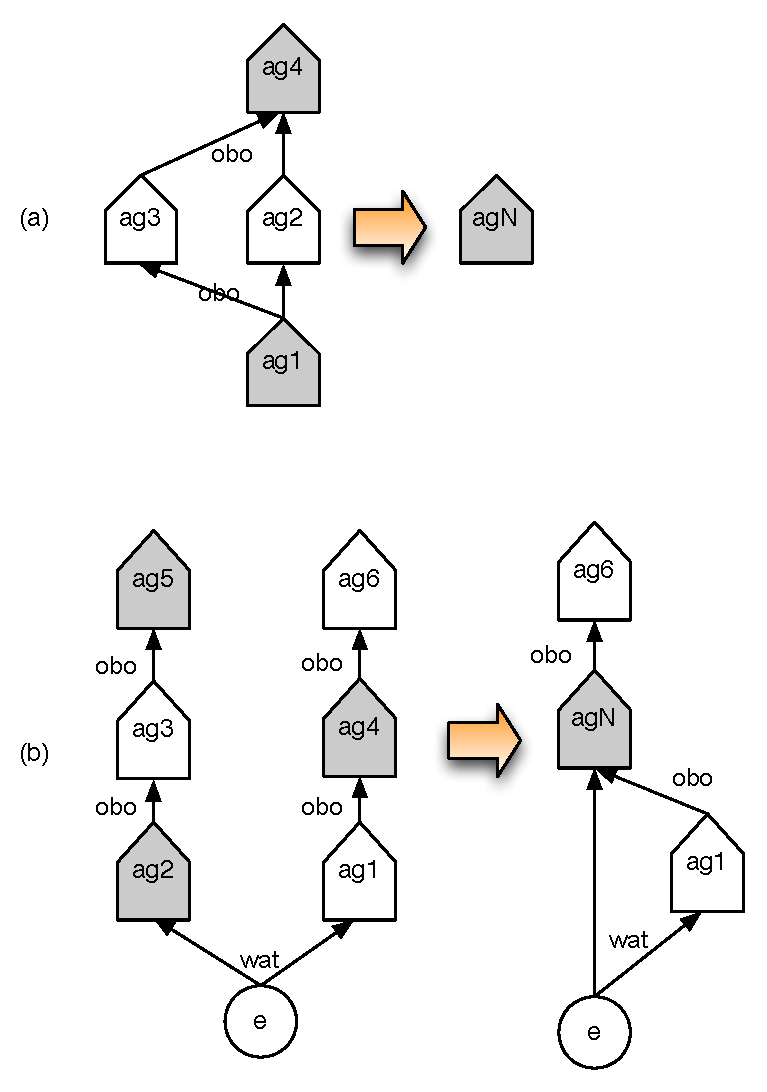
\includegraphics[scale=.5]{figures/d-chains-abstracted}
\caption{ag-grouping involving delegation.}
\label{fig:d-chains-abstracted}
\end{figure}

In pattern (b), $V_{gr} = \{ ag_2, ag_5, ag_4 \}$.
%
Note that not all agent nodes in $V_{gr}$ are related, either directly or through a path. This is not a problem, as we have $V_{clos} = \clos(V_{gr}, V) =   \{ ag_2, ag_5, ag_4, ag_3 \}$. Replacement applies as follows, where $\vartheta_{int}(V_{clos})$ is the set of relations beginning and ending inside $V_{clos}$:
\begin{eqnarray*}
\vartheta_{int}(V_{clos}) & = & \{ \delegate(ag_2, ag_3), \delegate(ag_3, ag_5) \} \\
\vartheta_{in}(V_{clos}) & = & \{ \wat(e, ag_2), \delegate(ag_1, ag_4) \} \\
\vartheta_{out}(V_{clos}) & = & \{ \delegate(ag_4, ag_6) \}
\end{eqnarray*}

% \begin{align*}
% &\vartheta_{int}(V_{clos}) = \{ \delegate(ag_2, ag_3), \delegate(ag_3, ag_5) \} \\
% &\vartheta_{in}(V_{clos}) = \{ \wat(e, ag_2), \delegate(ag_1, ag_4) \} \\
% &\vartheta_{out}(V_{clos}) = \{ \delegate(ag_4, ag_6) \}
% \end{align*}
% \

%
Thus, $\repl(V_{clos}, ag_N, G)$ maps relations in the original graph to those in the abstracted graph as follows:
%
\begin{eqnarray*}
\delegate(ag_4, ag_6) & \rightarrow &  \delegate(ag_N, ag_6) \\
\wat(e, ag_2) & \rightarrow &  \wat(e, ag_N) \\
\delegate(ag_1, ag_4) & \rightarrow &   \delegate(ag_1, ag_N)
\end{eqnarray*}

% \begin{align*}
% &\delegate(ag_4, ag_6) \rightarrow \delegate(ag_N, ag_6) \\
% &\wat(e, ag_2) \rightarrow \wat(e, ag_N) \\
% &\delegate(ag_1, ag_4) \rightarrow  \delegate(ag_1, ag_N)
% \end{align*}
% %
In practice, replacement preserves agents $ag_1$ and $ag_6$ and restores their delegation relations relative to the new abstract agent, $ag_N$. It also maps relation $\wat(e,ag_2)$, which involves the untouched $e$ node, to a new relation of the same type: $\wat(e,ag_N)$. 

We conclude that, in this first case, Def.~\ref{def:homo-group} applies without changes.

%\mnote{
%Points we must include somewhere
%\begin{itemize}
%  \item $V_{ag}$ means only type ag nodes included..
%  \item short forms of relations for general use
%  \item $\delegate(a,b) \in E$ means $(a,b) \in E \land label(a,b) = \delegate$
%  \item like-for-like: agents are abstracted to agents, not anything else.
%\end{itemize}
%}\\
%\mnote{
%  \begin{itemize}
%  \item close all delegate chains up, so we avoid cycles. ref sec on path closure.
%  \item remove and replace with $v_{new}$. 
%  \item rewire graph
%    \begin{itemize}
%    \item $\delegate$: agnets can't delagate to themselves \fbox{PM?}, otherwise retain delegate links
%    \item $\waw$ and $\wat$ remove all links: replace those that cross the abstract node boundary
%    \end{itemize}
%  \end{itemize}
%}
%

\subsection{a-grouping and e-grouping with agents}  \label{sec:t-grouping-agents}

The second case, where $V_{gr} \subset \en ~\cup~ \act$, is t-grouping with added agents relations.
%
Here the $\repl$ operator (Def.~\ref{def:group-replace}) must now consider how edges that involve agents are mapped to new edges in the abstract graph. 
%
We have already observed that agent nodes are always the targets of directed edges.
%
It follows that the closure of a set of nodes $V_{gr} \subset \en \cup \act$ never adds agent nodes to $V_{gr}$, because this would require the added agent to be on a path between two nodes from $\en ~\cup~ \act$, and therefore to be the source of a directed edge. 
%
%there can be no paths of the form $x \leftarrow ag \leftarrow y$  for $x,y \in \en \cup \act$.

%
A second observation is that if $\waw(a, ag)$ holds, and $a$ is involved in a-grouping, then $a$ is replaced by $a_{new}$, and thus $\waw(a_{new}, ag)$ also holds (Fig.~\ref{fig:agents-relations-patterns}(a1)).
%
Similarly for e-grouping, if $\wat(e, ag)$ holds, and $e$ is involved in e-grouping, then $e$ is replaced by $e_{new}$, and $\wat(e_{new}, ag)$ holds  (Fig.~\ref{fig:agents-relations-patterns}(b1)).
%
On the other hand, suppose $\waw(a,ag)$ holds and e-grouping is performed. A simple case is shown in Fig.~\ref{fig:agents-relations-patterns}(c1).
%
In this case, $a$ is replaced by $e_{new} \in \en$, therefore $\waw(e_{new},ag)$ is type-incorrect. Similarly, $\wat(e,ag)$ after a-grouping would become, incorrectly,  $\wat(a_{new}, ag)$.
%
These two patterns are summarised in Fig.~\ref{fig:agents-relations-patterns}(a2, b2 resp.). Note that one cannot simply replace association with attribution, i.e., replace relation $\waw(a, ag)$ with $\wat(e_N, ag)$, because there is no guarantee that any of the entities represented by the new $e_N$ had been attributed to $ag$ in the original graph. Similarly, one cannot replace $\wat(e, ag)$ with $\waw(a_N, ag)$.
%
Instead, in pattern (a) we simply remove the incorrect $\waw$ relations following e-grouping, and similarly, in pattern (b) we remove the incorrect $\wat$ relations following a-grouping.

\begin{figure}
\centering
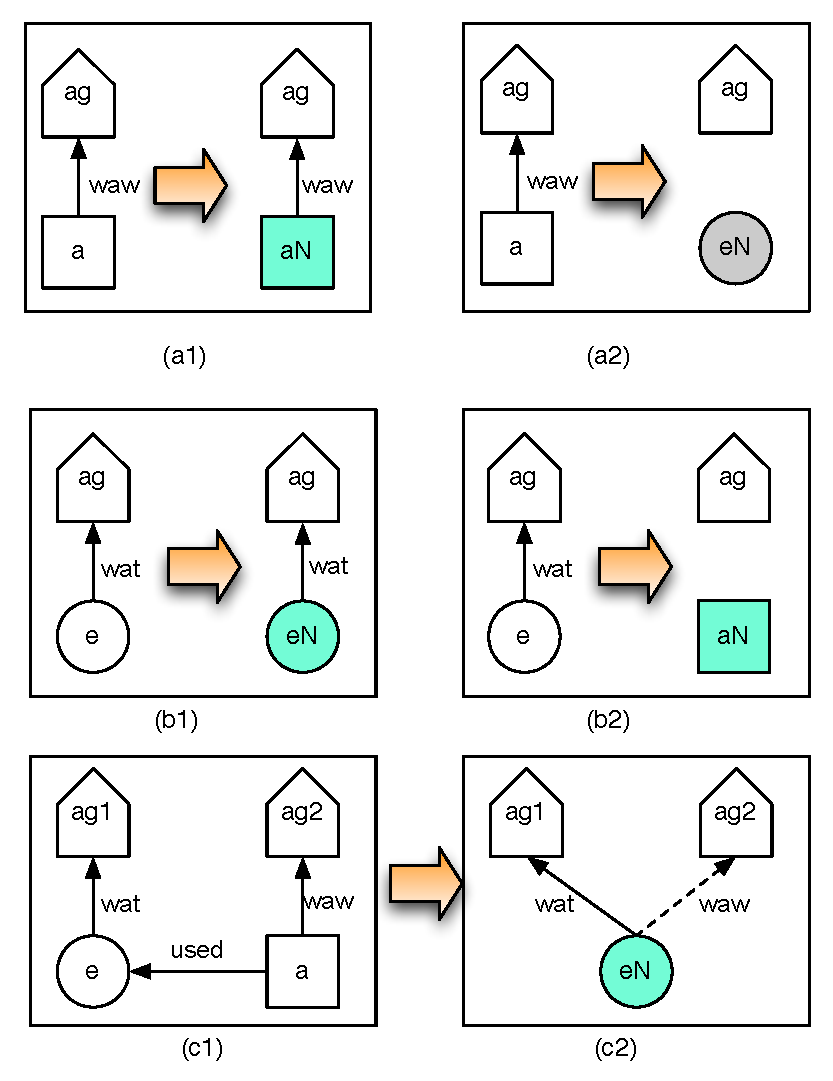
\includegraphics[scale=.5]{figures/agents-relations-patterns}
\caption{$\waw$ and $\wat$ edges involving nodes in $\clos(V_{gr}, V)$ may need to removed following e-grouping and a-grouping, respectively.}  \label{fig:agents-relations-patterns}
\end{figure}

%
These considerations suggest that the definition of the $\repl$ function for grouping needs to be adapted for the case where agents are involved. 
%
To understand why, recall from Sec.~\ref{sec:closure} that $\repl$ replaces a type-homogeneous set, computed by the $\extend$ function, with an abstract node of the same type. An extension of type $t$ augments the closure of a grouping set by adding all adjacent nodes of the same type to it. This ensures that replacing the nodes in the extension with an abstract node of the same type preserves the type correctness of the relations. 
%
However it should be clear from the example above (parts c1, c2 of the figure), that both e-grouping and a-grouping on the set  $V_{gr} = \{ a, e\}$  result in one of the two agent relations being incorrect. Intuitively, this is because the extension function fails to incorporate agents, leaving the agent relations exposed on the outcut of $V_{gr}$ (in fact, $\extend$ in this example does nothing at all).

The pattern in (c2) (or its symmetric, for a-grouping), can be obtained simply by ensuring that $\repl$ deletes the incorrect relations.
%
The following variation on Definition~\ref{def:eq:outcut} ensures these deletions are enforced.
\begin{align*}
\vartheta_{out}'(V_{gr}') = \{ & v \xleftarrow{t}  v_{new} |  v \xleftarrow{t} v' \in \vartheta_{out}(V_{gr}') ~\wedge \\
      ( & (t = \wat \wedge \type(v_{new}) = \en) ~\vee \\
        & (t = \waw \wedge \type(v_{new}) = \act)  ~\vee \\
        & (t \neq \wat \wedge t \neq \waw) )\} 
\end{align*}


%Agents may also be abstracted. Here, a naive approach raises again the problem of cycles in the graph.   To illustrate, suppose the agents $ag2$, $ag4$ and $ag5$ are to be abstracted from the two delegation chains in Figure~\ref{fig:d-chains-abstracted}. 
%
%
% 
%
%This leads to agent $ag3$ both delegating to and being a delegate of the abstract agent node $a''$, a situation which we disallow 
%
%\mnote{
%@PM there doesn't seem to be  a constraint that excludes this.  Should we disallow it?  Why/Why not?
%}
%
% 
%We introduce \emph{delegation chain closure}, which is akin to path closure and includes   agents which, although not part of the original request, must also be abstracted. 
%
%\begin{definition}[Delegate Chains]
%\label{def:del-chain}
%A \emph{delegate chain} is a directed chain of agents $a_1,a_2,\ldots,a_n$, such that $\forall i<n\spot \delegate(a_i,a_{i+1}) \in E$. 
%\end{definition}
%
%
%In Figure~\ref{fig:d-chains-abstracted}, agent $ag3$ must be included in the path.  The function $\dclos$, given in Definition~\ref{def:dclos}, is the result of restricting function $\clos$ (Definition~\ref{def:clos}) to operate only on agents and traverse only $\delegate$ links.
% 
%\begin{definition}[Delegate Chain Closure]
%\label{def:dclos}
%Let $G = (V,E) \in \guaEAG$ be a provenance graph, and let $V_{ag} \subset V$ be a set of agents.   
%For each pair  $a_i, a_j \in V_{ag}$ such that there is a delegate chain beginning at  $a_i$ and ending at $a_j$,  let $V_{ij} \subset V$ be the set of all nodes in the chain.
%The \emph{delegate chain closure} of $V_{gr}$ in $G$ is 
%\[\dclos(V_{ag}, G)  =  \bigcup_{v_i, v_j \in V_{ag}} V_{ij} \]
%\end{definition}
%
%
%For any set of agents $V_{ag}$ to be abstracted, $\dclos(V_{ag},G)$ returns the set of agents which need to be replaced by a new abstract agent.  Replacing these agents is again a similar task to the one carried out by the $\repl$ operator.
%
%
%\begin{definition}[Agents Replace]
%\label{def:agent-replace}
%\[ \agrepl(V_{ag}, ag_{abs}, G) = (V', E'), \mbox{ where: }\]
%\begin{align*}
%V' & = V \setminus V_{ag}  \cup \{ag_{abs}\} \\
%E' & = E \setminus & \\
%   & \{ \delegate(ag_{abs},ag)  | \\
%   & \quad  \exists ag' \in V_{ag} \spot ag \in V\hide V_{ag} \\
%   & \quad \land  \delegate(ag',ag) \in E \} \\
%   & \cup \{ \delegate(ag,ag_{abs})  | \\
%   & \quad \exists ag' \in V_{ag} \spot ag \in V\hide V_{ag} \land  \\
%   & \quad \delegate(ag,ag') \in E \} \\
%   & \cup \{ \waw(a,ag_{abs})| \\
%   & \quad \exists ag'\in V_{ag}\spot \waw(a,ag') \in E\}\\
%   & \cup \{ \wat(e,ag_{abs})| \\
%   & \quad \exists ag'\in V_{ag}\spot \wat(e,ag') \in E\}\\
%\end{align*}
%\end{definition}
%
%
%This definition replaces all relations between agents in the set $V_{ag}$ and agents in $V\hide V_{ag}$, and therefore we cannot create  orphan agents using $\agrepl$. 
%
%
%\begin{definition}[Grouping Agents]
%\label{def:ag-group-by}
%\begin{align*}
%\aggroup(G,V_{ag},ag_{abs}) = \agrepl(\dclos(V_{ag},G),ag_{abs},G) 
%\end{align*}
%
%\end{definition}


\subsection{The general case: grouping on any node type}

The third and more general case, where \mbox{$V_{gr} \subset \en ~\cup~ \act ~\cup~ \ag$}, presents one further  difficulty. Consider performing e-grouping on the pattern of Fig.~\ref{agents-baseline-obo-problem} (left), with \mbox{$V_{gr} = \{ e_4, ag_5 \}$}.
%
We have \mbox{$\clos(V_{gr}) = \{ e_4, ag_5, ag_3 \}$}, resulting in the abstraction on the right.
%
Clearly, the former $\delegate(ag_4, ag_3)$ relation should not be mapped in the final graph. 
%
This issue arises because there the extension function, which guarantees type consistency for e- and a-nodes, does not include agents. 
%

Once again we deal with the issue by changing the definition of $\repl$ to ensure that the incorrect relation is not mapped. 
%
Note that a change is required to $\vartheta_{in}'(V_{gr}')$ rather than $\vartheta_{out}'(V_{gr}')$ as in the previous case. The new definition is as follows.
\begin{align*}
\vartheta_{in}'(V_{gr}') = \{ & v_{new} \xleftarrow{t}  v |  v' \xleftarrow{t} v \in \vartheta_{in}(V_{gr}') \\
    & \wedge ( (t = \delegate \wedge \type(v_{new}) = \ag) \vee t \neq \delegate )\} 
\end{align*}
Thus, a delegation relation is mapped in the abstract graph only if the target abstract node is an agent.

\begin{figure}
\centering
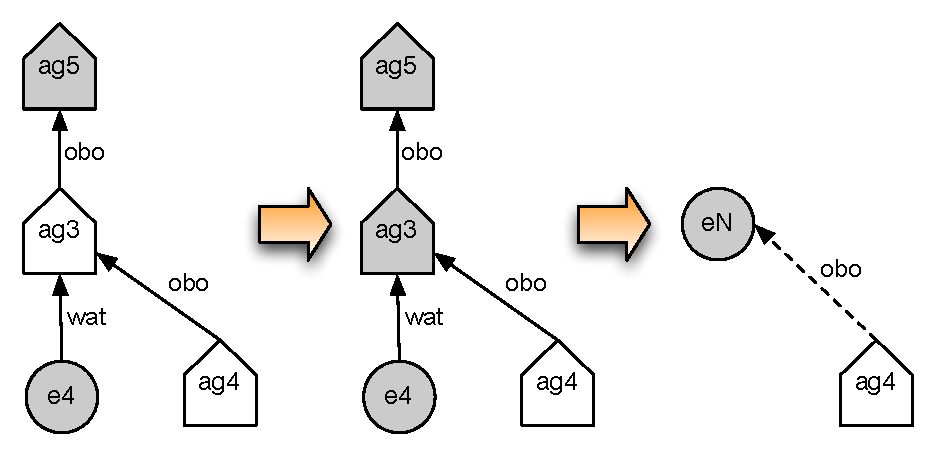
\includegraphics[scale=.5]{figures/agents-baseline-obo-problem}
\caption{e-grouping leads to incorrect $\delegate$ relation when agents are part of a closure.}
\label{agents-baseline-obo-problem}
\end{figure}

With the new version of the $\repl$ function, introduced in the previous two sections, some of the relations in the original graph $G$ are not mapped to the abstracted graph $G'$. This makes it possible for some of the nodes in $G'$ to end up disconnected from the rest of the graph. 
%
As an example, the graph in Fig.~\ref{agents-baseline-abstracted} shows the result of e-grouping over the shaded nodes in the graph of Fig.~\ref{fig:agents-baseline}. The combination of closure, extensions and replacement results in $ag_5$ being isolated, or ``orphaned'' in the abstract graph. 

%
As isolated agent nodes may not be significant to consumers of the abstracted graphs, for completeness we provide a simple function to optionally remove them at the end of the abstraction process, as follows.

\begin{figure}
\centering
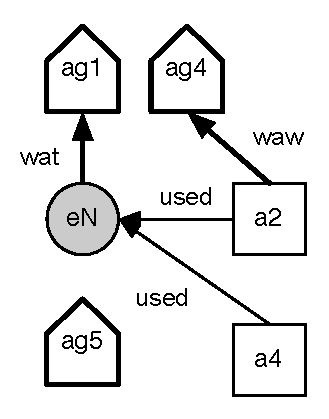
\includegraphics[scale=.5]{figures/agents-baseline-abstracted}
\caption{Abstracted version of the graph in Fig.~\ref{fig:agents-baseline} after e-grouping involving agents.}
\label{agents-baseline-abstracted}
\end{figure}


\begin{definition}[Removing isolated agents]
\label{def:orphanremove}
Let $G = (V,E) \in \guaEAG$, and 
\begin{align*}
 \mathit{isolated}(G) = \{  & v \in V | \type(v) = \ag \\
   & \wedge \nexists v' \in V . ((v',v) \in E \vee (v,v') \in E) \}
\end{align*}
Then:
\[ \remIsolated((V,E)) = (V \setminus \mathit{isolated}(G), E) \] 
\end{definition}




%\section{Tool Implementation}   \label{sec:summary}

Rather than giving a procedural pseudo-code for the $\group$ algorithm, we summarize its functional specification, comprising of the four functions defined so far: $\clos()$, $\extend()$, $\repl()$, and $\remIsolated()$, in Table~\ref{alg-summary}.

\begin{table*}
  \begin{eqnarray*}
    %%%%%%
    \clos(V_{gr}, V)  &%  
    = &%
     \bigcup_{v_i, v_j \in V_{gr}} V_{ij} \\
    %%%%%%
    \extend(V_{gr}, G ,t) &%
    = & V_{gr} 
      \begin{mydrop}
        ~\cup~ \{ v' | (v, v') \in E \wedge v \in V_{gr} \wedge \type(v') = t) \}  \\
        ~\cup~ \{ v | (v', v) \in E \wedge v \in V_{gr} \wedge \type(v') = t) \}  
      \end{mydrop} \\%
    %%%%%%
    \repl(V_{gr}, v_{new}, G) &% 
    = & %
    (V', E'), \mathrm{where}~~ 
       \begin{mydrop}
         \vartheta_{out}'(V_{gr}') = \{ v \xleftarrow{t}  v_{new} |  \begin{mydrop}
                 v \xleftarrow{t} v' \in \vartheta_{out}(V_{gr}')  \wedge \\%
                 ( (t = \wat \wedge \type(v_{new}) = \en) \vee \\%
                (t = \waw \wedge \type(v_{new}) = \act)  \vee \\%
                (t \neq \wat \wedge t \neq \waw) )\}  
              \end{mydrop} \\
         \vartheta_{in}'(V_{gr}') = \{  v_{new} \xleftarrow{t}  v | \begin{mydrop}
           v' \xleftarrow{t} v \in \vartheta_{in}(V_{gr}')  \wedge  \\%
           ( \begin{mydrop}
             (t = \delegate \wedge \type(v_{new}) = \ag) \\%
             \vee t \neq \delegate )\}
             \end{mydrop}
           \end{mydrop}
       \end{mydrop}\\
    %%%%%%
   V' & %
   = & %
   V  \setminus V_{gr}  \cup \{v_{new}\}  \\
    %%%%%%
   E' &% 
   = & % 
   E \setminus (\vartheta_{out}(V_{gr}) \cup \vartheta_{in}(V_{gr}) \cup \vartheta_{int}(V_{gr}))  \cup \vartheta_{out}'(V_{gr})  \cup \vartheta_{in}'(V_{gr}) \\
    %%%%%%
    \remIsolated(V,E) \mathrm{where} & %
    = &%
    (V', E') \\
    %%%%%%
    \mathit{isolated}(G) & 
    = & %
    \{  v \in V | \type(v) = \ag  \wedge \nexists v' \in V . ((v',v) \in E \vee (v,v') \in E) \} \\
    V' & %
    = & %
    V \setminus \mathit{isolated}(G)\\
    %%%%%%
    E' &
    =&
    E \\
    %%%%%%
    \group(G, V_{gr}, v_{new}, t) &%
    = & %
    \remIsolated(\repl( \extend(\clos(V_{gr},V), V, t), v_{new},  G ))
    %%%%%%
  \end{eqnarray*}
  \caption{Functional summary of the grouping algorithm.}
  \label{alg-summary}
\end{table*}



% \begin{table*}
% \begin{tabularx}{\textwidth}{lXlX}
% %%%%%%
% $\clos(V_{gr}, V) $ &  
% %%%%%%
% $ \bigcup_{v_i, v_j \in V_{gr}} V_{ij}$ \\
% %%%%%%
% $\extend(V_{gr}, G ,t) = V_{gr}:$ &  
% %%%%%%
% $\cup \{ v' | (v, v') \in E \wedge v \in V_{gr} \wedge \type(v') = t) \}  
% \cup \{ v | (v', v) \in E \wedge v \in V_{gr} \wedge \type(v') = t) \} $ \\
% %%%%%%
% $\repl(V_{gr}, v_{new}, G) = (V', E'):$ &  
% $\vartheta_{out}'(V_{gr}') = \{ v \xleftarrow{t}  v_{new} |  v \xleftarrow{t} v' \in \vartheta_{out}(V_{gr}')  \wedge ( (t = \wat \wedge \type(v_{new}) = \en) \vee 
% (t = \waw \wedge \type(v_{new}) = \act)  \vee (t \neq \wat \wedge t \neq \waw) )\} $ \newline
% $\vartheta_{in}'(V_{gr}') = \{  v_{new} \xleftarrow{t}  v |  v' \xleftarrow{t} v \in \vartheta_{in}(V_{gr}')  \wedge ( (t = \delegate \wedge \type(v_{new}) = \ag) \vee t \neq \delegate )\} $ \newline
% $V' = V  \setminus V_{gr}  \cup \{v_{new}\} $ \newline
% $ E' = E \setminus (\vartheta_{out}(V_{gr}) \cup \vartheta_{in}(V_{gr}) \cup \vartheta_{int}(V_{gr}))  \cup \vartheta_{out}'(V_{gr})  \cup \vartheta_{in}'(V_{gr}) $\\
% %%%%%%
% %%%%%%
% $\remIsolated(V,E) = (V', E')$ & 
% $\mathit{isolated}(G) = \{  v \in V | \type(v) = \ag  \wedge \nexists v' \in V . ((v',v) \in E \vee (v,v') \in E) \}$ \newline
% $V ' = V \setminus \mathit{isolated}(G), E' =  E$ \\
% %%%%%%
% $\group(G, V_{gr}, v_{new}, t):$&
% $\remIsolated(\repl( \extend(\clos(V_{gr},V), V, t), v_{new},  G ))$
% \end{tabularx} 
% \caption{Functional summary of the grouping algorithm.}
% \label{alg-summary}
% \end{table*}
% 
 
A procedural implementation of the algorithm, written in Java, is available online (\url{https://github.com/PaoloMissier/ProvAbs}) as part of a tool in which a policy language is used to drive the selection of the set $V_{gr}$ of nodes to be abstracted. Using the tool, policy setters may experiment with abstraction policies on their provenance graphs, observing their effects when abstraction is performed.
%
Noting that $\group()$ is closed wrt composition, the tool also allows for more complex abstraction, by letting users specify compositions of $\group$ operations as part of their policy.

%
Here we only provide a brief description of the tool. A more detailed account can be found in~\citep{Missier2013c} (submitted).
%
The tool operates on provenance graphs written in the provenance notation PROV-N~\citep{w3c-prov-n}.

%
Given $G \in \guaEAG$, the tool lets users specify a grouping set $V_{gr}$ by means of an \textit{abstraction policy}. It operates in two steps. Firstly, path expressions and predicates are used to select a set of nodes, and to assign a numerical \textit{sensitivity} value to them. 
%
For example, the following rule contains a path expression that binds variables \texttt{process} and \texttt{data} to activity and entity nodes $a$, $e$, respectively, such that $\used(a,e)$ holds and $e$ is any node that is reachable from node with id \texttt{d14}:

\vspace{0.5\baselineskip}

\small
\textsf{for all (process used data)}

\textsf{ \;\;\; where (data descendantOf d14)) }

\textsf{ \;\;\;\;\;\; setSensitivity(data, 10)}

\vspace{0.5\baselineskip}

\normalsize

The sensitivity value of the selected data nodes is set to 10.
%
Here \textit{descendantOf} is a built-in query predicate that returns all nodes reachable from a given start node. 

%
As an another example, the  predicate

\vspace{0.5\baselineskip}

\small
\textsf{for all (data wgb process)} 

 \textsf{ \;\;\; where (process.classification $>$ ``conf'' in classifications) }

\textsf{ \;\;\;\;\;\; setSensitivity(data, 9)}

\vspace{0.5\baselineskip}

\normalsize


binds variables \texttt{data} and \texttt{process} to pairs of nodes $d$, $p$ such that $\wgby(d,p)$ and where the classification value $p.classification$ of $p$ (a property of the node) is greater than ``conf''. This requires an ordered set of classification labels to be declared in a user-defined \texttt{classifications} list.
%
During the first step, the tool evaluates the policy rules, resulting in the annotation of the selected nodes with sensitivity values. 

%
This model operates on the same principle as the Bell-LaPadula security model. Each known receiver of a graph is pre-assigned a clearance level. This is determined by factors outside the scope of the tool, e.g. how much a receiver is trusted to the provenance owner. 
%
In the second step, node sensitivities are compared to the clearance level $cl$ of the receiver, and $V_{gr}$ is defined as the set of nodes whose sensitivity is lower than $cl$.
%

The rationale for these two steps is that sensitivity can be defined largely independently of the specific receiver, while the exact level of abstraction is relative to a receiver, who in this case is represented simply by a clearance level.

%Such predicates 
%For example, if certain activities had a property named \emph{sensitivity} which contained numeric values, then ``\emph{all entities produced by processes that sensitivity} $\ge$ \emph{5}'' is a valid clause within the policy language.  
%
%
%
%The evaluation of a policy over $G$ results in the identification of the set of nodes $V_{gr}$. The user can then  apply $\group(G, V_{gr}, v_{new}, t)$ to a graph $G \in \guaEAG$, where $t$ is again selected by the user. 
%



\section{Summary and further research}
\label{sec:further}

We have proposed a model for the principled obfuscation of provenance based on a formal definition of abstraction, in which sensitive elements of a provenance graph are grouped together and replaced with a single abstract node.  The presentation is incremental: first we develop the model for the case when the nodes of provenance graphs are restricted to entities and activities, and then consider the case where nodes may also be agents.  A guiding principle  throughout is that we avoid the introduction of \emph{false dependencies}: abstraction will reduce the information content of a provenance graph, but it will not introduce false information.  
The abstraction acts on and results in provenance graphs which are PROV compliant.   A separate paper presents the tool implementing this model in detail.


The work described in this paper is progressing in two main directions.
%
First, we are aware that the fragment of PROV to which this version of $\group$ applies does not cover all relation types. Nevertheless, the method described in the paper for reasoning about PROV graph transformation can be used as a guideline to extend the work to the missing parts of PROV. We are going to address these in the future.

Second, so far we have ignored the implications of abstraction on the space of events that are used to characterize the semantics of PROV. As constraints over the relative ordering of events are defined in detail in the PROV-CONSTR document, there is however an obligation to extend the notion of validity of PROV graphs to include those constraints. Thus, grouping must be shown to be validity-preserving relative to those constraints as well. 

\comment{Address: The authors have not considered what domains enforce a validity constraint and what if it is relaxed to show an partially inconsistent graph?}



\section*{Acknowledgements}

The support of the ONRG and the EPSRC in funding this research is gratefully acknowledged. 

\section*{References}

\bibliographystyle{plain}
\bibliography{prov-abstraction-foundations}

\appendix

%\section{Proofs}
\subsection{The function $\col$}
\mnote{still to do:
\begin{itemize}
  \item calc edges of $E_{21}$ and show equal to $E_{12}$.
  \item whole proof of equality of nodes. 
  \item so $(G_{12} = G_{21})$. 
\end{itemize}
}




$\col$ collapses the path between two nodes, and replaces it with a new node. All edges into or out of the path are relabeled according to the function $\relabel$.
  
\begin{definition}[$\col$]  \label{def:col}
  For nodes $x$, $y$ in a graph $G = (V,E)$, and a new node $v_{N}$ not in $V$,  $\col(x,y,G)$ is defined provided there is a path between nodes $x$ and $y$. Let $P$ be the set of all nodes on the path from $x$ to $y$. Let $r(l)$ stand for the function $\relabel(l)$. Then $\col(x,y,G) =  (V',E')$, where 
  \begin{eqnarray*}
  V' & = & (V\hide P) \union \{v_N\}     \\
  E' & = & E\hide (
                   \{(v',v,l)|(v',v,l) \in in(v), v\in P\}
                   \union
                   \{(v,v',l)|(v,v',l) \in out(v), v\in P\}
                  )\\
  && \union\ \{(v',v_{N},r(l))|(v',v,l) \in in(v), v\in P\}\\
  && \union\ \{(v_{N},v',r(l))|(v,v',l) \in out(v), v\in P\}\\
  \end{eqnarray*}
\end{definition}
If $type(v)$ returns the type of a node $v$, the function $relabel$ (abbreviated above as $r$) is defined as 
\begin{definition}[$relabel$] \label{def:relabel}
  For an edge $(v,v',l)$, 
  \[
   (v,v',relabel(l)) = \left\{
   \begin{array}{l}
      l,    {\emph{if}}\; type(v) \neq type(v') \\
      infl, \emph{otherwise}
   \end{array}   \right.
  \]
\end{definition}
\noindent
$relabel$ is promoted in the obvious way to sets of edges. 

To show that  the order of application of two $\col$ functions does not matter, (ie. that $\col$ commutes with itself)  we need to show that for any nodes $w,x,y,z$ in a graph $G$, $\col(y,z,\col(w,x,G)) = \col(w,x,\col(y,z,G))$. 


We begin with some definitions.

$P_1$ is defined as $\Path(w,x)$.

$P_2$ is defined as $\Path(y,z)$.

$\{v_i\} = \Path(x,w) \inter \Path(y,z)$. Note that in general this is a set of nodes. 



%$E_1$ is the set of nodes after $\col(w,x,G)$ has been carried out.

%$E_2$ is the set of nodes after $\col(y,z,G)$ has been carried out.

% If the new node resulting from $\col(y,z,G)$ is $v_{N1}$,

%$P'_1$ is the path between $w$ and $x$ \textbf{after} $\col(y,z,G)$ has been carried out, resulting in the new node $v_{N1}$. It is defined $P'_1 = (P_1\hide\{v_i\})\union\{v_{N1}\}$.  

%Similarly,  $P'_2$ is the path between $y$ and $z$ \textbf{after} $\col(w,x,G)$ has been carried out, resulting in the new node $v_{N2}$.  It is defined as $P'_2 = (P_2\hide\{v_i\})\union\{v_{N2}\}$.  



We  calculate the nodes and edges of  $\col(y,z,\col(w,x,G))$,  then $\col(w,x,\col(y,z,G))$, showing that they both result in the same final graph. For readability, we introduce simplifying definitions through the proof. 


Edges:

Following the definitions recorded above, $\col(w,x,G)$ results in graph $G_1=(V_1,E_1)$, where

\begin{eqnarray*}
  E_1 & = & E\hide (
                   \{(v',v,l)|(v',v,l) \in in(v), v\in P_1\}
                   \union
                   \{(v,v',l)|(v,v',l) \in out(v), v\in P_1\}
                  )\\
  && \union\ \{(v',v_{N},r(l))|(v',v,l) \in in(v), v\in P_1\}\\
  && \union\ \{(v_{N},v',r(l))|(v,v',l) \in out(v), v\in P_1\}\\
\end{eqnarray*}

\noindent
We now introduce the simplifying definitions:
\[
 in(P_1)   = \{(v',v,l)|(v',v,l) \in in(v), v\in P_1\} \\ 
 out(P_1)  = \{(v,v',l)|(v,v',l) \in out(v), v\in P_1\}\\
 in(v_{N1}) = \{(v',v_{N1},r(l))|(v',v,l) \in in(v), v\in P_1\} \\
 out(v_{N1})= \{(v_{N1},v',r(l))|(v,v',l) \in out(v), v\in P_1\} \\
\]
\noindent
With a slight abuse of notation, $in(\{v_{N1}\})$ (resp. $out(\{v_{N1}\})$)  is written $in(v_{N1})$ (resp. $out(v_{N1})$). These simplifies the definition of $E_1$ to 
\[
  E_1  = ( E\hide(in(P_1) \union out(P_1)) ) \union ( in(v_{N1}) \union out(v_{N1}) )
\]
\noindent  
$P_1$ and $P_2$ intersect (on the nodes $\{v_i\}$), so we record the modification in $P_2$ \textbf{after} $\col(w,x,G)$ has been carried out as

It is defined as $P'_2 = (P_2\hide\{v_i\})\union\{v_{N1}\}$.  If $v_f$ is the replacement abstract node, then


\begin{eqnarray*}
  E_{12} =  & = & E_1\hide (
                   \{(v',v,l)|(v',v,l) \in in(v), v\in P'_2\}
                   \union
                   \{(v,v',l)|(v,v',l) \in out(v), v\in P'_2\}
                  )\\
  && \union\ \{(v',v_f,r(l))|(v',v,l) \in in(v), v\in P'_2\}\\
  && \union\ \{(v_f,v',r(l))|(v,v',l) \in out(v), v\in P'_2\}\\
\end{eqnarray*}

\noindent
We  introduce some more simplifying definitions:
\[
in(P'_2) = \{(v',v,l)|(v',v,l) \in in(v), v\in P'_2\}\\
out(P'_2) = \{(v,v',l)|(v,v',l) \in out(v), v\in P'_2\}\\
in(v_f) = \{(v',v_f,r(l))|(v',v,l) \in in(v), v\in P'_2\}\\
out(v_f) = \{(v_f,v',r(l))|(v,v',l) \in out(v), v\in P'_2\}\\
\]
\noindent
allowing us to re-write the defintion of $E_{12}$ as
\[
  E_{12}  =  (E_1\hide ( in(P'_2) \union out(P'_2)))  \union\ (in(v_f) \union out(v_f))
\]
  

\noindent
and then (by substitution of the $E_1$) as


\[
E_{12}  =  \left( \left(
\begin{array}{l}  E\hide(in(P_1) \union out(P_1)) \\  \union \\ (in(v_{N1}) \union out(v_{N1}) ) \\
\end{array} \right)
   \hide ( in(P'_2) \union out(P'_2)) \right) \\
\hphantom{E_{12}  = \;\; }   \union\ \\
\hphantom{E_{12}  = \;\;}   (in(v_f) \union out(v_f))\\ 

\]

\noindent
and then, by substitution of $P'_2$

\[
E_{12}  =  \left( \left(
  \begin{array}{l}
    E\hide(in(P_1) \union out(P_1)) \\  \union \\ (in(v_{N1}) \union out(v_{N1}) ) \\
  \end{array} \right)
   \hide
   \left( \begin{array}{l}
     in((P_2\hide\{v_i\})\union\{v_{N1}\}) \\\union\\ out((P_2\hide\{v_i\})\union\{v_{N1}\})
   \end{array}
   \right) \right) \\
   \hphantom{E_{12}  = \;\; }   \union\ \\
\hphantom{E_{12}  = \;\;}   (in(v_f) \union out(v_f))\\ 
\]

\noindent
then, since $(P_2\hide\{v_i\}) \inter \{v_{N1}\} = \emptyset$, by distributing $in$ and $out$ over $\union$, we get  

\[
E_{12}  =  \left( \left(
  \begin{array}{l}
    E\hide(in(P_1) \union out(P_1)) \\  \union \\ (in(v_{N1}) \union out(v_{N1}) ) \\
  \end{array} \right)
   \hide
   \left( \begin{array}{l}
     in(P_2\hide\{v_i\})\union in(\{v_{N1}\})) \\\union\\ out(P_2\hide\{v_i\})\union out(\{v_{N1}\})
   \end{array}
   \right) \right) \\
   \hphantom{E_{12}  = \;\; }   \union\ \\
\hphantom{E_{12}  = \;\;}   (in(v_f) \union out(v_f))\\ 
\]

\noindent
We can therefore remove $out(\{v_{N1}\})$ and $out(\{v_{N1}\})$ from both sides of the set hiding operator, leaving 

\[
E_{12}  =  \left( \left(
  \begin{array}{l}
    E\hide(in(P_1) \union out(P_1)) \\  
  \end{array} \right)
   \hide
   \left( \begin{array}{l}
     in(P_2\hide\{v_i\}) \\\union\\ out(P_2\hide\{v_i\})
   \end{array}
   \right) \right) \\
   \hphantom{E_{12}  = \;\; }   \union\ \\
\hphantom{E_{12}  = \;\;}   (in(v_f) \union out(v_f))\\ 
\]
\noindent
and, since $\{v_i\}$ is the set of intersection nodes, and therefore $\{v_i\} \subseteq P_1$, we can write

\[
E_{12}  =  
   E\hide
  (
    in(P_1) \union out(P_1) \union in(P_2) \union out(P_2)
  ) \\
   \hphantom{E_{12}  = \;\;}   \union\ \\
\hphantom{E_{12}  = \;\;}   (in(v_f) \union out(v_f))\\ 
\]

Now, we  revisit the defintion of $v_f$. and compare to $v_g$...

Below, we expand the definition of $in(v_f)$. $out(v_f)$ an exercise!

\[
in(v_f) = \{(v',v_f,r(l))|(v',v,l) \in in(v), v\in P'_2\}
\]
\noindent
by defition of $P'_2$,
\[
in(v_f) = \{(v',v_f,r(l))|(v',v,l) \in in(v), v\in((P_2\hide\{v_i\})\union\{v_{N1}\})\}
\]
\noindent
and,  simplification, 
\[
in(v_f) = \{(v',v_f,r(l))|(v',v,l) \in in((P_2\hide\{v_i\}) \union \{v_{N1}\})\}
\]
\noindent
and, by set manipulation, 
\[
in(v_f) = \{(v',v_f,r(l))|(v',v,l) \in in(P_2\hide\{v_i\}) \union  \{(v',v_{N1},r(l))|(v',v,l)\in in(v), v\in P_1\}\}
\]
\noindent
which, by definition of $in(P_1)$, we can write as
\[
in(v_f) = \{(v',v_f,r(l))|(v',v,l) \in in(P_2\hide\{v_i\}) \union  r(in(P_1))\}
\]
\noindent
where $r(in(P))$ is the relabeling operator $r$ promoted to sets.  Which, since $r$ is idempotent ($r(r(l)) = r(l)$), we can write as
\[
in(v_f) = \{(v',v_f,r(l))|(v',v,l) \in in(P_2\hide\{v_i\}) \union  in(P_1)\}
\]
\noindent
and since $\{v_i\} \subseteq P_1$, 
\[
in(v_f) = \{(v',v_f,r(l))|(v',v,l) \in in(P_2) \union  in(P_1)\}
\]

\mnote{still need to repeat this for $E_{21}$ and show two results are equal. This proof might be best in a TR version}

\pagebreak


%\section{Multiple applications of $\repl$.}
\label{app:multiple}

We begin by recalling the definition of the function $\repl$.
\begin{definition}[replace]
\label{def:group-replace}

\[ \repl (V^*, v_{new}, G) = (V', E'), \mbox{ where: } \]
\begin{eqnarray*}
V' & = & V  \setminus V^*  \cup \{v_{new}\}\\
E' & = & E  \setminus (\vartheta_{out}(V^*) \cup \vartheta_{in}(V^*) \cup \vartheta_{int}(V^*))  \\
   & & \qquad \cup\  \vartheta_{out}'(V^*)  \cup \vartheta_{in}'(V^*)
\end{eqnarray*}
\end{definition}


We need to show that the order in which $\repl$ is carried out is irrelevant, i.e., if $v_n$ and $v_m$ are the new nodes, we need to show that
\[
\repl(V_b,v_m,\repl(V_a,v_n,G)) = \repl(V_a,v_n,\repl(V_b,v_m,G))
  \]
  


  
%\subsection{Proof}

%To show that  the order of application of the two $\repl$ functions does not matter,   we need to show that given a graph $G=(V,E)$,    $\repl(V_b,v_m,\repl(V_a,v_n,G)) = \repl(V_a,v_n,\repl(V_b,v_m,G))$.
  
\vspace{10pt}
{\bf Approach to proof}
\vspace{10pt}

We  calculate the edges and nodes of
$\repl(V_b,v_m,\repl(V_a,v_n,G))$, then the edges and nodes of
$\repl(V_a,v_n,\repl(V_b,v_m,G))$, 
showing that they both result in the same final graph.
%



  
 
\subsection*{Equality of nodes}

We first show that for $ G=(V,E); V_a,V_b \subseteq V$; $I=V_a\inter V_b$  and $V_n,V_m \nin V$, the nodes resulting from 
$\repl(V_b,v_m,\repl(V_a,v_n,G))$, and the nodes resulting from 
$\repl(V_a,v_n,\repl(V_b,v_m,G))$ are equal.

We begin by calculating the nodes of $\repl(V_a,v_n,G)$.
%
Following the definition of $\repl$ reproduced above, $\repl(V_a,v_n,G)$ results in the nodes $V_1$, where 

\begin{eqnarray*}
  V_1 & = & V\hide V_a \union \{v_n\}
\end{eqnarray*}

At this point, $V_b$ is modified, so let $V'_b = V_b$ after $\repl(V_a,v_n,G)$, ie $V'_b = V_b\hide I \union \{v_n\}$. The final set of nodes, which we denote $V_{12}$, is given by $V_{12} = V'_b\hide I \union \{v_f\}$. We use $v_f$ as the name for the final set of nodes to emphasise the fact that this will be different from $v_m$. Similarly, when we carry out the $\repl$ functions in the other order, we will use $v_g$ for the name of the final set of nodes. $v_f$ and $v_g$ are not in $V$. 

\[
V_{12} \\
= \\
V_1\hide V'_b \union \{v_f\}\\
= (\rm{by~replacing~} V'_b) \\
V_1\hide\ (V_b\hide I \union \{v_n\}) \union \{v_f\}\\
= (\rm{by~replacing~} V_1) \\
(V\hide V_a \union \{v_n\})~\hide\ (V_b\hide I \union \{v_n\}) \union \{v_f\}\\
= (\rm{by~removing~} v_n)\\
(V\hide V_a)~\hide\ (V_b\hide I) \union \{v_f\}\\
= (\rm{since~} I=V_a \inter V_b)\\
(V\hide V_a)~\hide\ (V_b) \union \{v_f\}\\
=\\
V\hide (V_a \union V_b) \union \{v_f\}
\]

A similar argument holds for $V_{21}$, showing $V_{21} = V\hide (V_a \union V_b) \union \{v_g\}$ and so $V_{21}=V_{12}$ (up to $\alpha$-equivalence).


\subsection*{Equality of edges}


To show that the edges remain unchanged in either order, we begin by calculating the edges of $\repl(V_a,v_n,G)$.
%
Following the definition of $\repl$ reproduced above, $\repl(V_a,v_n,G)$ results in graph $G_1=(V_1,E_1)$, where

\begin{eqnarray*}
  V_1 & = & V\hide V_a \union \{v_n\}\\
  E_1 & = & E\hide ( \INN(V_a) \union \OUT(V_a) \union \INT(V_a)) \\
  && \union\ \{(v',v_{n})|(v',v) \in \INN(V_a) \}\\
  && \union\ \{(v_{n},v')|(v,v') \in \OUT(V_a) \}\\
\end{eqnarray*}

and we define
\[
\INN(v_n) = \{(v',v_n)|(v',v) \in \INN(V_a) \}\\
\OUT(v_n) = \{(v_n,v')|(v,v') \in \OUT(V_a) \}
\]

\noindent  
Let $I = V_a \inter V_b$.  We record the modification in $V_b$ \textbf{after} $\repl(V_a,v_n,G)$ has been carried out as $V'_b = (V_b\hide I)\union\{v_{n}\}$.
If, following both applications of $\repl$,  $v_f$ is the final replacement abstract node, $V_{12}$ is the final set of nodes and $E_{12}$ is the final set of edges, then

\begin{eqnarray*}
  V_{12} & = & V_1 \hide V'_b \union \{v_m\} \\
  E_{12} &  = & E_1\hide ( \INN(V'_b) \union \OUT(V'_b) \union \INT(V'_b) )\\
  && \union\ \{(v',v_{f})|(v',v) \in \INN(V'_b) \}\\
  && \union\ \{(v_{f},v')|(v,v') \in \OUT(V'_b) \}
\end{eqnarray*}
\noindent
where we define 

\[
% in(P'_2) = \{(v',v,l)|(v',v,l) \in in(v), v\in P'_2\}\\
% out(P'_2) = \{(v,v',l)|(v,v',l) \in out(v), v\in P'_2\}\\
 \INN(v_f) = \{(v',v_f)|(v',v) \in \INN(V'_b) \}\\
 \OUT(v_f) = \{(v_f,v')|(v,v') \in \OUT(V'_b) \}
 \]
 \noindent
 By substitution of the $E_1$, we get: 

\[
E_{12}  =  \left( \left(
\begin{array}{l}  E\hide(\INN(V_a) \union \OUT(V_a) \union \INT(V_a)) \\  \union \\ (\INN(v_n) \union \OUT(v_n) ) \\
\end{array} \right)
   \hide ( \INN(V'_b) \union \OUT(V'_b) \union \INT(V'_b) ) \right) \\
\hphantom{E_{12}  = \;\; }   \union\ \\
\hphantom{E_{12}  = \;\;}   (\INN(v_f) \union \OUT(v_f))
\]
\noindent
and then, by substitution of the $V'_b$ (recall $V'_b$ is the modification made to $V'_b$ by the first $\repl$ operation: $V'_b = (V_b\hide I)\union\{v_{n}\}$):

\[
E_{12}  =  \left( \left(
\begin{array}{l}  E\hide(\INN(V_a) \union \OUT(V_a) \union \INT(V_a)) \\  \union \\ (\INN(v_n) \union \OUT(v_n) ) \\
\end{array} \right)
\hide    \left( \begin{array}{l}
  ( \INN((V_b\hide I)\union\{v_{n}\})~ \union\ \\ \OUT((V_b\hide I)\union\{v_{n}\})~ \union\ \\ \INT((V_b\hide I)\union\{v_n\}) ) 
         \end{array}
         \right) \right) \\
\hphantom{E_{12}  = \;\; }   \union\ \\
\hphantom{E_{12}  = \;\;}   (\INN(v_f) \union \OUT(v_f))\\ 
\]

\noindent
then, since $(V_b\hide I) \inter \{v_{n}\} = \emptyset$, we can distribute $\INN$ and $\OUT$  over $\union$. Furthermore,  $\INT(v_n) = \emptyset$, since $v_n$ is a single node.

\[
E_{12}  =  \left( \left(
\begin{array}{l}
  E\hide(\INN(V_a) \union \OUT(V_a) \union \INT(V_a)) \\  \union \\ (\INN(v_n) \union \OUT(v_n) ) \\
\end{array} \right)
   \hide
   \left( \begin{array}{l}
     \INN(V_b\hide I)\union \INN(v_n) ~\union\ \\
     \OUT(V_b\hide I)\union \OUT(v_n)  \\
     \INT(V_b\hide I)) 
   \end{array}
   \right) \right) \\
   \hphantom{E_{12}  = \;\; }   \union\ \\
\hphantom{E_{12}  = \;\;}   (\INN(v_f) \union \OUT(v_f))\\ 
\]

\noindent
We can therefore remove $\INN(\{v_n\})$ and $\OUT(\{v_n\})$ from both sides of the set hiding operator, leaving 

\[
E_{12}  =  \left( \left(
  \begin{array}{l}
  E\hide(\INN(V_a) \union \OUT(V_a) \union \INT(V_a)) ) \\
  \end{array} \right)
   \hide
   \left( \begin{array}{l}
     \INN(V_b\hide I) ~\union\ \\
     \OUT(V_b\hide I) ~\union\ \\
          \INT(V_b\hide I)) 
%     \INT(V_b\hide I)\union \INT(\{v_n\}) 
   \end{array}
   \right) \right) \\
   \hphantom{E_{12}  = \;\; }   \union\ \\
\hphantom{E_{12}  = \;\;}   (\INN(v_f) \union \OUT(v_f))\\ 
\]


\noindent
and, since $I = V_a \inter V_b$,  and therefore $I \subseteq V_a$, we can write

\[
E_{12}  = 
  E\hide(\INN(V_a) \union \OUT(V_a) \union \INT(V_a) \union    \INN(V_b) ~\union \OUT(V_b)   ~\union   \INT(V_b\hide I))  \\
   \hphantom{E_{12}  = \;\; }   \union\ \\
\hphantom{E_{12}  = \;\;}   (\INN(v_f) \union \OUT(v_f))\\ 
\]


Next, observe that, since $I \subseteq V_b$, $V_b\hide I = V_b$, and so  $\INT(V_b\hide I) = \INT(V_b)$. 

\[
E_{12}  = 
  E\hide(\INN(V_a) \union \OUT(V_a) \union \INT(V_a) \union    \INN(V_b) ~\union \OUT(V_b)   ~\union   \INT(V_b))  \\
   \hphantom{E_{12}  = \;\; }   \union\ \\
\hphantom{E_{12}  = \;\;}   (\INN(v_f) \union \OUT(v_f))\\ 
\]


A similar chain of reasoning to the above demonstrates that


\[
E_{21}  = 
  E\hide(\INN(V_a) \union \OUT(V_a) \union \INT(V_a) \union    \INN(V_b) ~\union \OUT(V_b)   ~\union   \INT(V_b))  \\
   \hphantom{E_{21}  = \;\; }   \union\ \\
\hphantom{E_{21}  = \;\;}   (\INN(v_g) \union \OUT(v_g))\\ 
\]


It now remains to show that the edges associated with $v_f$ and $v_g$ are teh same: ie that $\INN(v_f) = \INN(v_g)$ and $\OUT(v_f) = \OUT(v_g)$.

Consider $\INN(v_f)$. We know that $ \INN(v_f) = \{(v',v_f)|(v',v) \in \INN(V'_b) \}$, and by expansion of the definition of $V'_b$ we get
\[
\INN(v_f) \\
=\\
\{(v',v_f)|(v',v) \in \INN(V_b\hide I \union \{v_n\}) \}\\
=\\
\{(v',v_f)|(v',v) \in \INN(V_b\hide I) \union \INN(\{v_n\}) \}\\
=\\
\{(v',v_f)|(v',v) \in \INN(V_b\hide I)\} \union \{(v',v_f)|(v',v)\in \INN(\{v_n\}) \}\\
=(\rm{by~~definition~~of~~}\INN(\{v_n\})\\
\{(v',v_f)|(v',v) \in \INN(V_b\hide I)\} \union \{(v',v_f)|(v',v)\in \{(v',v_n)|(v',v) \in \INN(V_a)\} \}\\
=(\rm{by~~simplication})\\
\{(v',v_f)|(v',v) \in \INN(V_b\hide I)\} \union \{(v',v_f)|(v',v) \in \INN(V_a)\} \}\\
=(\rm{since~~} I=V_a\inter V_b)\\
\{(v',v_f)|(v',v) \in \INN(V_b)\} \union \{(v',v_f)|(v',v) \in \INN(V_a)\} \}\\
=\\
\{(v',v_f)|(v',v) \in \INN(V_b) \union \INN(V_a) \}\\
\]


Similar reasoning shows that $\INN(v_g)$ also is equal to $\{(v',v_g)|(v',v) \in \INN(V_a)\union \INN(V_b) \}$, and thus the $\INN(v_f) = \INN(v_g)$.

The demonstration that $\OUT(v_f) = \OUT(v_g)$ follows similar lines.


  
 




\end{document}
